
\documentclass[11pt,openany]{book}
\usepackage{wrapfig}
%\usepackage{graphics}
\usepackage{color}
\usepackage[usenames,dvipsnames]{xcolor}
\usepackage{titlesec}
\usepackage{makeidx}
\usepackage{graphicx}
\usepackage{epsfig,subfigure}
\usepackage{fullpage}
\usepackage{enumerate}
\usepackage{listings}
\makeindex

\title{A Project-Based Introduction to C++}
%\date{Date}
\date{}
\author{\\ \\ Terence Soule\\ \\ \\University of Idaho}


\begin{document}
\maketitle

\frontmatter

\tableofcontents

\newcommand{\codefont}[1]{\texttt{#1}}
\newcommand{\cf}[1]{\texttt{#1}}

%\titleformat{\chapter}
%{\color{blue}\normalfont\LARGE\bfseries}
%{\color{blue}\thechapter}{1em}{}

\newif\ifcolor
\colortrue
\newcommand{\mycolor}{Mahogany}


\newcommand{\mysubsubsection}[1]{\vspace{-0.25cm}\subsubsection{#1}\vspace{-0.25cm}}
%\newcommand{\mysubsubsection}[1]{\vspace{0.25cm}\textbf{#1}}

\newcommand{\mysubsection}[1]{\vspace{-0.25cm}\subsection{#1}\vspace{-0.25cm}}

\newcounter{modNumber}
\newcommand{\modification}[1]{\vspace{0.25cm}
{\noindent{\large\textbf{Mod \arabic{chapter}.\arabic{modNumber}: #1\\}}}}


\newcounter{interlude}
\newcommand{\interlude}[1]{\newpage{\noindent{\LARGE\textbf{Interlude \arabic{interlude}: #1}}}
\addcontentsline{toc}{chapter}{Interlude \arabic{interlude}:  #1}\\\\}


\newenvironment{tight_itemize}{
\vspace{-0.2cm}
\begin{itemize} 
\setlength{\itemsep}{2pt} 
\setlength{\parskip}{0pt} 
\setlength{\parsep}{0pt} 
}{\end{itemize}}

\newenvironment{tight_enumerate}{
\vspace{-0.25cm}
\begin{enumerate} 
\setlength{\itemsep}{2pt} 
\setlength{\parskip}{0pt} 
\setlength{\parsep}{0pt} 
}{\end{enumerate}}

\mainmatter
%********** Acknowledgments **********
\chapter*{Acknowledgments}

Many thanks to Joshua Rubini who was a great advocate of the project-based approach and wrote preliminary versions of several of the programs.  Without his early enthusiasm this text would never have been written.  Thanks to Dr. Clinton Jeffery  for being brave enough to teach from a preliminary version of the text and whose suggestions were extremely helpful in refining the text.  Finally, thanks to the Spring 2013 CS120 class at the University of Idaho, whose keen eyes caught many typos and whose sharp minds made many helpful suggestions.
%********** End of acknowledgements **********

%\addtocounter{chapter}{1}
%********** Chapter 1 **********
\chapter{Introduction}

%Computer programs are used for an amazing array of tasks: helping to fly airplanes and drive cars, creating intricate games, controlling robots that learn, running complex simulations of the natural world, creating incredibly life-like - or completely imaginary - worlds.  All of these depend on the programs running inside the computers.  Programmers 

Computer programming is fundamentally a creative activity. 
Programmers use the elements of a programming language as the building blocks to write programs for almost any task they can imagine, from games to complex simulations to robots capable of learning to incredibly lifelike -- or completely imaginary -- worlds.   Programmers are always experimenting with ways to improve their programs, to make them more interesting, more efficient, or easier to use.  Thus,
programming requires imagination and experimentation. This text is designed to encourage the creative, hands-on, and experimental aspects of programming while teaching the fundamentals of the C++ programming language.

Typically, anyone wanting to learn a new skill, like woodworking or electronics, begins by building projects designed by someone else.  Then, as they become more confident, they start modifying those projects, experimenting with changes to make them better or to meet their own goals.  Eventually, they start creating their own projects from scratch.  Similarly, beginning artists often go to museums to learn by copying the masters and then experiment with applying their own styles.  Architects learn by studying existing designs and then experimenting with their own variations.  The common idea in all of these approaches is learning through imitation and experimentation.  

Computer programming is particularly well-suited to this style of learning.  Not only can programs be studied; they can be copied, modified, tested, remodified, and, if things go badly, reverted back to the original -- an artist can't do that with the \emph{Mona Lisa}.
This text is designed to support this experimentation-based style of learning, emphasizing the creative, experimental aspects of programming.  Each of the following chapters is divided into three main sections.  The first section introduces the major programming elements covered in the chapter and presents a complete program, starting with the game of NIM in Chapter 2, that demonstrates how those programming elements are used.  The second section analyzes the program line by line, explaining what each line does and how it contributes to the overall program.  The third section discusses different ways to modify and improve the program, beginning with simple changes and detailed instructions and ending with suggestions for much more complex modifications.   After each project chapter, there is a short ``interlude'' covering general topics useful to the reader: debugging, testing, design, etc.

This approach to learning to program has many strengths -- and some limitations.  It makes it possible to begin working with interesting programs right away.  It encourages experimentation, creativity, and an active, hands-on approach to programming.  It supplies a working program that readers can always go back to if their changes fail or if  they want to try something new.

However,  because each chapter focuses on the sample program, they contain fewer of the details of C++ syntax.  To balance this, the Appendix supplies details that are intentionally missing from the main chapters.  Thus, in each chapter, there are pointers to sections in the Appendix that explain specific topics in more detail.  Some readers may be more comfortable with lots of experimentation and learning on their own (and won't be as bothered by programs that often don't do what's expected) and will use the Appendix less. Other readers may want to spend more time understanding the details and will refer to the Appendix often.  Each reader should take the approach that works best for him or her.

\section{Programming}

\emph{Programming} is the process of writing a program that a computer can run.  A program is really just a set of instructions, like a recipe.  One of the most difficult aspects of programming is that computers are completely literal.  A chef can put the instruction ``add three eggs'' in a recipe and be fairly confident that anyone following the recipe will actually break the three eggs, add just the egg, and throw away the shells.  A computer would need to be told explicitly to break the eggs and throw away the shells.  Thus, an important part of  learning to program is learning to describe tasks in very precise, well-defined steps.  

A programming language is a specific set of basic instructions that can be combined to create a program.  Different languages often represent the same instruction in different ways.  Table~\ref{tab:instructions} gives some examples of how the instruction: \codefont{x = y + 7} might appear in different languages.  In each language the general structure of the command is similar, but the details vary.

\begin{table}[ht]
\centering
\begin{tabular}{|l|l|}
\hline
C++ & x = y + 7; \\
\hline
Pascal & x := y + 7; \\
\hline
Perl & \$x = \$y + 7; \\
\hline
\end{tabular}
\caption{The command \codefont{x = y + 7} as it is written in different programming languages.}
\label{tab:instructions}
\end{table}

Very broadly, programming languages are divided into low-level languages\index{low-level language} and high-level languages\index{high-level language}.  Low-level languages are relatively hard for people to understand, but easier for computers to understand.  High-level languages are easier for people to understand, but further from what a computer can understand.  C++ is a high-level language, although arguably at the lower end of the high-level languages; C++ is easier for people to understand than a low-level language, but perhaps not by a lot.

Because computers cannot directly execute a program written in a high-level language (i.e., they cannot ``understand'' a program written in a high-level language), a \emph{compiler}\index{compiler}  or an \emph{interpreter}\index{interpreter}\index{interpreted language} is necessary to ``translate'' a program written in a high-level language into a language the computer can understand.  A compiler translates an entire program, creating a complete program the computer can actually run -- often called an ``executable.''  There are a variety of interpreters, but a common form of interpreter translates a program one line at a time, as the computer is running the program.  Interpreted programs run much slower than compiled programs because the computer has to wait for each line to be translated as it's running, rather than having the entire translation done in advance.  

Because C++ is a compiled language, programs are written using a text editor or an Integrated Development Environment (IDE)\index{Integrated Development Environment}\index{IDE} and then the program is compiled to create an executable program.\footnote{Interpreters for C++ do exist and can be useful for some tasks, but they are not very common and will not be covered in this text.}  The initial program is really just a text document (although it usually has an extension like \codefont{.cpp} to indicate that it represents a program).  The compiled program is a file that the computer can actually run.  These files are often called \emph{executables} because the computer can execute them (as in ``execute an order'').  

%When a C++ program is compiled the resulting executable file can typically only run on computers with a similar operating system to the one it was compiled on.  So, if you write a C++ program and compile on a computer running Windows 7 the compiled program may not run on a computer running Windows Vista.  However, if you take the original C++ program and compile on the computer running Windows Vista, then it should run there.\footnote{There are ways to make an executable more platform independent, but they are a bit complicated and won't be discussed here.}

IDEs usually include a text editor specialized for writing programs and built-in tools for automating the compiling process.  IDEs often make programming easier because they automatically format and color-code a program, help identify errors, and even make suggestions.\footnote{If you are using an IDE like Visual Studio, all of the programs in the text can be entered as \emph{console applications}.}  Commonly used IDEs include Microsoft Visual Studio, Eclipse, and Netbeans.   Visual Studio includes a free Express version and Eclipse and Netbeans are free and can be downloaded from the Web. 

%Why C/C++(?)

\section{Using This Text}

Begin each chapter by reading the introductory sections.   These explain what the chapter's program does and what new programming concepts it introduces.  After reading those sections enter the program.  Once the program is entered, compile it and run the program.  Run each program a few times, examining how it works, and trying different inputs.  By comparing the program's behavior to the program's code, it is often possible to understand at least some of how the program works.  

After you have entered and run a program a few times, you should begin reading the section of the chapter explaining the major features of the program.  This should help you further understand how the program works.

Once you have a general feeling for what the program does, start reading the analysis of the code.  While reading  the code analyses in each chapter, add comments to the code (see Chapter 2 for more information on comments) to make it more understandable.  

While reading about the code, it is often useful to rerun the program to see how the description of the code compares to what the program is actually doing.  Try changing the program to see if the changes make the program behave in the expected way -- just remember to keep a backup copy of the original program so you don't have to completely reenter the program if it ``breaks.'' 

Keep in mind that at this point, it is almost completely impossible to write a program that would damage the computer in any way.  At worst, a program that won't compile or ``crashes'' when run -- in which case the program can simply be reverted to the backup version that works.  So, feel free to experiment.

After you feel like you understand how the original program works, it's time to start really modifying it.  Each chapter has several sections presenting suggested modifications.  The first modifications are simple, carefully described changes that should be easy to implement and will improve, at least a little, how the program functions.  The later modifications are more complex and less detailed; this is where you really test yourself.  

Remember, experiment, try your own ideas, and most of all, have fun.


%********** End of chapter **********


%\addtocounter{chapter}{1}
\setcounter{section}{0}
\setcounter{figure}{0}
%********** Chapter 1b, the new chapter 2 **********

\chapter{Fortune Teller}\label{ch:fortune}\index{Fortune Teller}\index{projects!Fortune Teller}

%\section{Introduction}

This chapter dives into programming with the first project, a program that generates a user's lucky number and uses it to predict the user's fortune\index{Fortune Teller}.  The program works by asking the user for a favorite and a disliked number and then combines them to create a lucky number and a fortune based on the lucky number.  As we'll see the program is fairly simple, but also very flexible. It's possible to include all sorts of user input and fortunes.

The Fortune Teller program introduces the following elements of programming:
\begin{tight_itemize}
   \item Comments\index{comments}
   \item Variables\index{variables}
   \item Input/output (I/O)\index{I/O}
   \item Mathematical Expressions\index{Expressions}
   \item Conditionals:\index{conditionals} \cf{if}
   \item Libraries\index{libraries}
\end{tight_itemize}

Comments are sections of code used by the programmer to make the program more readable, but that are ignored by the computer, that is they are comments about the code from one programmer to another.   Variables are used to store the data used by a program.  Input is data that comes into a program from another source -- typically the keyboard or a file.  Output is data that is sent from a program -- typically to the screen or to a file.  Mathematical expressions let the program perform mathematical operations.
Conditionals are specialized commands that allow a program to make a ``decision'' -- doing one thing under some conditions and doing something else under other conditions.  Without conditionals programs would always do exactly the same thing.   
Libraries are sets of prewritten code that are included in a program.  As the Fortune Teller project demonstrates, a basic understanding of these elements is sufficient for writing  fairly sophisticated and interesting programs.

\section{The Program}

Listing~\ref{listing:FortuneTeller} presents the code for the Fortune Teller.  Notice that the program is actually fairly short -- only 38 lines long -- and many of the lines are comments.  When entering the code do \emph{not} enter the line numbers along the left side of the program.  Those are just for reference.  As the program is entered, try to figure out what the commands do.  Most will be difficult to understand at this point, but some of them may make sense.

%\begin{figure}
\begin{minipage}{\textwidth}
\begin{lstlisting}[language=C++,numbers = left, xleftmargin=4.0ex, basicstyle=\small,emph={num_objects,move,current_player},emphstyle = \color{\mycolor},
showstringspaces=false,
caption = {The code for the Fortune Teller.  When entering this program, do not enter the line numbers.  Keywords (also known as reserved words) are in bold, comments are in italics, and variables are colored maroon.}]
      /* The Fortune Teller -
       * a simple program introducing some
       * fundamental programming concepts.
       */
#include <iostream>  // include a library
using namespace std;
int main()  // main() starts the program
{
	// ----------------- Variable declarations ------------------------
	int favorite;  // create a variable to store the favorite number
	int disliked;  // create a variable to store the disliked number
	int lucky;  // create a variable to store the lucky number
	// ----------------- Get user input -----------------------------
	cout << "Enter your favorite number (no decimals): ";  // output
	cin >> favorite;                         // user input
	cout << "Enter a number you don't like (no decimals): ";
	cin >> disliked;
	// Next calculate the user's lucky number
	lucky = (favorite * disliked) % 10;
	cout << endl << "Your secret, lucky number is: " << lucky << endl;
	if(lucky < 0){  // conditional, values less than 0
		cout << "Try to be less negative." << endl;
	}
	if(lucky >= 0 && lucky < 5){ // 0 to 4 inclusive
		cout << "Think bigger!" << endl;
	}
	if(lucky >= 5 && lucky < 9){  // 5 to 8 inclusive
		cout << "Today you should embrace technology." << endl;
	}
	if(lucky == 9){     // exactly 9
		cout << "Today is your lucky day!" << endl;
	}
	// ------- Code to help the program exit "gracefully" --------
	cin.ignore();
	cout << "Press enter to quit." << endl;
	cin.ignore();
	return 0;
}
\end{lstlisting}\label{listing:FortuneTeller}
\end{minipage}
%\caption{The code for NIM.  When entering this program, do not enter the line numbers.}
%\end{figure}\label{fig:NIM1}



\begin{wrapfigure}{R}{0.5\textwidth} \vspace{-0.5cm}\framebox[\linewidth][l]
{\parbox{0.96\linewidth}
{\textbf{Using Comments} \\
Good code contains many comments.  Comments make code much more readable, which makes it easier to understand, modify, and expand a program.  Most of the programs presented in this text are seriously \emph{under}-commented so that the reader can add their own comments as the meaning of the code becomes clearer.  This is done to encourage the reader to add comments to the code.  It also saves space and reduces the amount of text to copy (although the comments can be skipped when the program is entered).  Software companies often have rules that specify how code must be commented (for example, requiring a comment before every function).  If you are using this text as part of a course, there are likely requirements that each program start with a block comment containing information like your name, the assignment number, and your section.
}}
\vspace{-1.5cm}
\end{wrapfigure}

Once the entire program has been entered, compile it.  Depending on how carefully the program was entered, the compiler may generate some error messages.  Try to fix them and compile the program again.  Read the compiler error messages carefully; at the very least, they report the line that the error occurred on.  Because one error may hide another error, it may take several iterations of compiling and fixing errors before the program compiles successfully.  More detailed suggestions on how to fix a program that's not compiling or running properly are presented in the interlude following this chapter.

Once the program compiles, run it a few times to generate different fortunes.  While running the program compare the program's output to the program's code.  It should be possible to recognize what many of the program statements do by seeing how the program runs.  

Running the program will also reveal that it has some shortcomings.  It doesn't tell the user what the program does.  The output messages are not always clear.  There's a fairly limited number of fortunes.   These are shortcomings that we will eventually want to fix.  But before modifying the program it is necessary to discuss its important elements and to analyze how it works.

\subsection{Comments}\index{comments}

 A \emph{comment} is part of a program that has no effect on how a program runs, but that makes a program more readable for humans, either by explaining what a section of code does or by structuring the program so that it is easier to read.  For example, the comments on lines 5 and 7 explain those lines of code and the comments on lines 9, 13, and 33 serve to break the program into three easy-to-identify blocks.  

Comments are defined in C++ in two ways, either using two slashes // (e.g., lines 9, 10, and 11) or with a /* ... */ pair (lines 1-4).  When two slashes are used, everything from the slashes to the end of the line is a comment.  For example, the first part of line 10, up to the slashes, is regular code and the rest, after the slashes, is a comment.
When a /* ... */ pair is used, everything from the starting /* to the ending */ is part of the comment.  For example, the block of text on lines 1-4 is one large comment.

\subsection{Variables}\index{variables}

Programs often need to keep track of information -- the program's \emph{data}.  For example, the Fortune Teller needs to know the user's favorite, disliked, and lucky numbers.  Programs use \emph{variables} to keep track of this information.  A variable can be thought of as a named box that stores a piece of data.  Figure~\ref{fig:variables1} illustrates this idea.

\begin{wrapfigure}{R}{0.5\textwidth}\vspace{-0.5cm} \framebox[\linewidth][l]{\parbox{0.96\linewidth}
{
\codefont{Naming Variables} \\
The rules for valid variable names are fairly simple.  Variable names can use letters, underscores (\_), and digits, but cannot start with a digit and must contain at least one letter.   They may not be a reserved word, such as \codefont{if}, \codefont{int}, or \codefont{main}.  In the code listings reserved words are shown in bold.  Case matters: \codefont{X} is not the same variable as \codefont{x}.  Thus, legal variable names include: \codefont{X}, \codefont{a\_variable}, and \codefont{variable7}, but \emph{not} \codefont{7variable} (starts with a digit),
% \codefont{\_123} (doesn't contain a letter),
or \codefont{do} (a reserved keyword).  There are a number of conventions for choosing variable names and software companies often enforce the use of a particular convention.  Several  conventions are used in this text to demonstrate the range of variable naming styles.
}   }
\vspace{-0.4cm}
\end{wrapfigure}

In addition to its name, each variable must have a \emph{type}\index{type}.   The type defines what kind of data can be stored within a variable.  The Fortune Teller program has three variables: \cf{favorite}, \cf{disliked}, and \cf{lucky}, all of which have the same type: integer or \cf{int}.  There are three main reasons why a program  must know the type of a variable.  First, the type determines how ``big'' a variable's box is -- literally, how much of the computer's memory it takes up.  

\begin{figure}
%\centerline{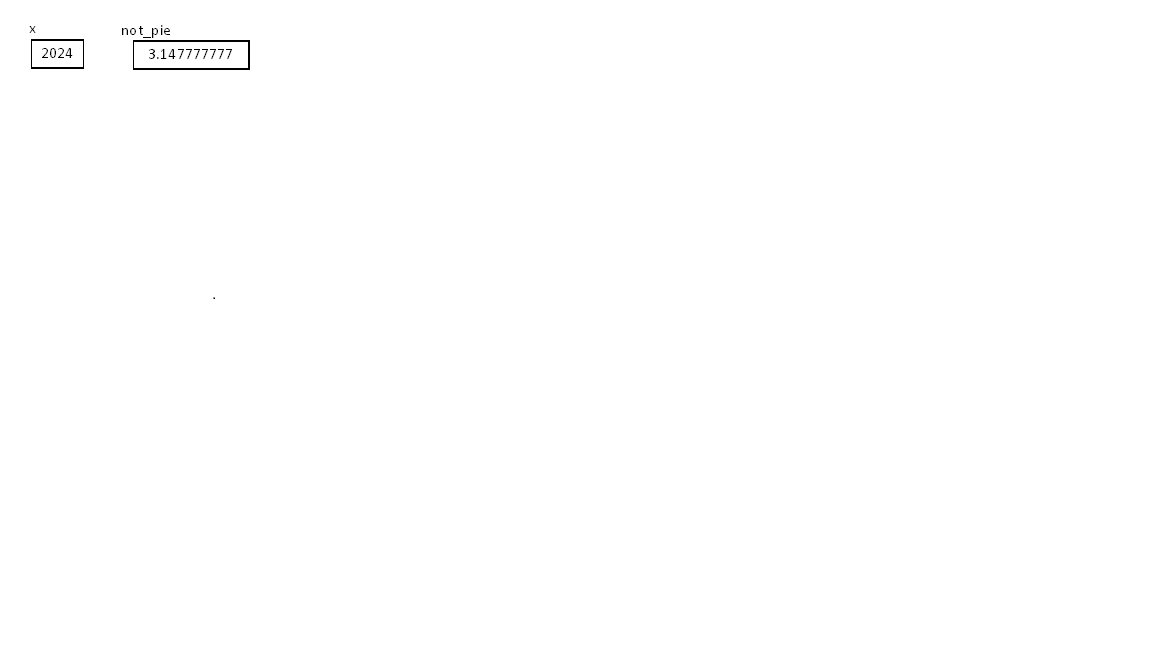
\includegraphics[width=9cm,height=3cm]{images/variables.bmp}}
\setlength{\unitlength}{1cm}
\begin{picture}(10,2)

\linethickness{0.3mm}

\put(4.2,1.1){376}
\put(4,1.7){\codefont{X}}
\put(7.2,0.9){4.17222}
\put(7,1.5){\codefont{not\_pi}}

\put(10.2,0.7){f}
\put(10,1.3){\codefont{character\_variable}}

\color{\mycolor}{
\put(4,1){\line(1,0){1}}  % bottom
\put(4,1.5){\line(1,0){1}} % top
\put(4,1){\line(0,1){0.5}} % left
\put(5,1){\line(0,1){0.5}} % right

\put(7,0.8){\line(1,0){2}}  % bottom
\put(7,1.3){\line(1,0){2}} % top
\put(7,0.8){\line(0,1){0.5}} % left
\put(9,0.8){\line(0,1){0.5}} % right

\put(10,0.6){\line(1,0){0.5}}  % bottom
\put(10,1.1){\line(1,0){0.5}} % top
\put(10,0.6){\line(0,1){0.5}} % left
\put(10.5,0.6){\line(0,1){0.5}} % right
}

\end{picture}
\caption{Variables can be thought of as boxes with a name that hold a value.  Different types of variables correspond to different-sized boxes. }
\label{fig:variables1}
\end{figure}

Second, the type determines how to interpret the data stored in the variable.  At the lowest level, data is stored in a computer as a binary\index{binary} number.  \emph{Binary numbers} are numbers that are written using only the digits 0 and 1, instead of the digits 0 to 9 we are used to (see Appendix~\ref{appendix:binary}).  
Computers use binary numbers because they can use \codefont{off} and \codefont{on} to represent 0 and 1.  However, different data types use the 0's and 1's in different ways.  The computer needs to know the type of the variable to know how to interpret the 0's and 1's stored in the variable.

Third, the type tells the program how operations should be applied to the data stored in the ``box.''  For example, when division is applied to two integers, the answer is an integer and the remainder is ignored, but when division is applied to two real numbers the answer is also a real number.

Variables are declared using statements like:\\
\codefont{
\emph{type} name;\\
\emph{type} name1, name2, name3;\\
\emph{type} name4 = \emph{value};\\}
where the \codefont{\emph{type}} is the type of the variable to be created, \codefont{name} is the name of the ``box,'' and \codefont{\emph{value}} is the value the variable initially stores.  
The second of these statements demonstrates that multiple variables can be declared in one statement, as long as all of the variables have the same type.  The third statement shows that variables can be assigned a value as soon as they are created.
For the Fortune Teller, only variables of type \emph{integer}\index{integer}\index{type!int@{\cf{int}}} (abbreviated as \codefont{int} in C++\footnote{Computer languages and computer programmers often rely on abbreviations.}) are used.  Other types are introduced in later chapters, and Section~\ref{appendix:types} in Appendix A has a list of the most commonly used types in C++.  In the Fortune Teller variables are declared (i.e., created) on lines 10-12.

Variable names are selected by the programmer, subject to C++'s naming rules (see the text box Naming Variables).   Giving variables meaningful names makes code easier to read and understand. For example, the variable holding the user's favorite number is named \cf{favorite}. 

\subsection{Input and Output}\index{I/O}

In C++, input and output to a program goes through objects known as  \emph{streams}\index{streams}.  A stream object represents a device that can send or receive data using input and output operations.  For example, \codefont{cout} is a stream object representing the computer terminal, so sending data to \codefont{cout} results in the data being displayed on the screen.  

Data is sent to or received from streams using stream \emph{operations}.  Most stream operations have a similar structure: they define the stream to be used and the type and/or amount of data to be sent or received.  In C++ the most common stream operators are $<<$ and $>>$, which represent sending data to or receiving data from a stream.  For example, the statement:\\
\codefont{cout $<<$ "Hello, world!";}\\
sends the data in the string ``Hello, world!'' to the stream \codefont{cout}. Thus, this command prints the words ``Hello, world!'' on the screen.  Many other streams and stream operations exist and will be introduced throughout the text.  A list of the most common stream operations is included in Section~\ref{appendix:iostream} of Appendix A. 

\subsection{Expressions}\index{expressions}

Mathematical expressions are simply used to perform calculations within a program.  Their general format is:\\
\cf{x = \emph{mathematical expression}}\\
where \cf{x} is a variable and the \emph{mathematical expression} is build from variables, numbers, and mathematical operators (+, -, etc.).  The variable \cf{x} is assigned the value that is calculated on the right hand side of the expression.  

There are a two things to be careful of when creating mathematical expressions in C++: \emph{order of operations} and \emph{types}.  Order of operation is the order that mathematical operations are applied in a compound mathematical expression like:\\
\cf{x = y + 7 * 8 - z}\\
C++ uses the standard rules for order of operation (multiplication and division before addition and subtraction; addition and subtraction are performed left to right; etc.).  So, in the previous expression \cf{7 * 8} would be performed first.  %However, C++ includes a number of useful, but possibly unfamiliar, mathematical operations (See Section~\ref{appendix:operators} of Appendix A) whose

C++ has many mathematical operators, including basic operators like addition (+), subtraction (-), and division ($\backslash$), and more unusual, but useful, mathematical operations like increment (++) and decrement (- -).  More operators will be introduced as they are needed in later chapters.  Section~\ref{appendix:operators} of Appendix A has a list of the commonly used C++ operators.  Because the order of operations of these operators may not be familiar it is a good idea to use parentheses to force operations to take place in the desired order.  Including parentheses also makes expressions easier to read.

Depending on the types involved mathematical expressions can sometimes give unexpected results.  For example, the code:\\
\cf{
int x = 8;\\
cout << x / 10;\\
}
prints the number \emph{0}.  The variable \cf{x} and number 10 are both integers, so C++ treats the answer as an integer and the value 0.8 (possibly the expected answer) is \emph{truncated}\index{truncation} to zero.  There are a number of ways to avoid this problem.  For example, if the code were rewritten as:\\
\cf{
int x = 8;\\
cout << x / 10.0;\\
}
including the decimal on 10.0 tells C++ to treat the answer as a decimal and the code will print 0.8.  The issue of types in mathematical operations is examined in more detail in later chapters when more types (besides \cf{int}) have been introduced.

\subsection{Conditionals: \cf{if}}\index{conditionals}

Conditionals allow a program to choose between two (or more) options.  The options are often referred to as \emph{branches}.  One of the most common conditionals is the \emph{if}\index{if@{\cf{if}}} statement.  All conditionals have a \emph{condition}\index{condition}: if the condition is true the computer executes (i.e., runs) one block of code, if the condition is false the program skips that block of code, and may run a different block of code instead.  The format of an if statement is:\\
\codefont{
if(\emph{condition}) \{\\
\hspace*{0.5cm}Execute this block of code\\ 
\hspace*{0.5cm}if the condition is true\\
\}\\
Always executed\\
}
Notice that the condition is inside the parentheses after the \codefont{if}.  The blocks of code within the if statement is denoted in two ways: it is surrounded by curly braces, \{ and \}, and the code is indented.  The curly braces define the block of code within the if statement for the computer.  Whereas the indenting makes it easier for programmers to quickly identify the code that is part of the if statement.  Indenting is not required, but blocks of code within curly braces should \emph{always} be indented because it makes the code much easier to read.  


C++ also has an if-else statement and a switch statement both of which are slightly more complex conditionals, covered in later chapters.  These conditional statements are also summarized in Section~\ref{appendix:conditionals} of Appendix A.  

Conditions used in conditional statements are typically written as \emph{Boolean} expressions.  Boolean expressions are logical expressions whose value is either \emph{true} or \emph{false}.  Boolean expressions are constructed by using comparison operators like less than ($<$), greater than ($>$), equal to ($==$), and not equal to ($!=$).  Boolean expressions also use the logical operators AND (which is written as $\&\&$ in C++), OR (written as $||$), and NOT (written $!$).  For example, the 
statement:\\
\cf{
x < y || y > z \\
}
is a condition that is true \emph{if x is less than y OR if y is greater than z}. 
Commonly used comparison and logical operators are introduced in later chapters and summarized in Section~\ref{appendix:Boolean} of Appendix A.  

Although Boolean expressions evaluate to true or false, C++ takes a shortcut and uses a \cf{0} for false and a \cf{1} for true.  For example, a command like:\\
\codefont{cout << (6 < 8) << endl;}\\
will print a 1 because 6 is less than 8 and C++ uses a 1 for true and 0 for false.  Similarly, the expression \codefont{6 > 8} would produce a 0.  

More generally, in C++ any nonzero value is treated as true.  This means that non-Boolean expressions can be used in conditions.  For example, the condition in an if-else statement could be \codefont{x - 7}.  This would be interpreted as ``false'' for \codefont{x = 7} because \codefont{x - 7} would be 0.  It would be interpreted as ``true''; for any other value of \codefont{x}.  However, using mathematical operations in the place of comparisons is generally a poor idea because it makes the code less readable.  For example, understanding the condition \codefont{x - 7} is harder than understanding \codefont{x != 7} even though both test the same condition.  


\section{Analysis of the Code}

This section analyzes the code in Listing~\ref{listing:FortuneTeller} line by line.  It explains how the program works and how the statements in the program can be modified or used in other programs.  The goal in analyzing the code is to understand the Fortune Teller program and to understand how the statements used in Fortune Teller can be adapted for writing other programs.

\mysubsubsection{Lines 1-5, 7, and More: Comments}
Because computer programs are generally difficult for humans to read, comments are included to make programs more readable to humans.  In C++ there are three general forms of comments: block comments, full line comments, and end of line comments. 
Lines 1-4 are a single block comment describing the program.  Block comments begin with a /* and end with a */, anything between those two symbols are ignored by the complier.  Note that the extra *'s on lines 2 and 3 are not required, they are there just to make the comment easier to identify.  Programmers often include contextual cues to make different parts of a program easier to see.

\begin{wrapfigure}{R}{0.5\textwidth} \vspace{-0.3cm} \framebox[\linewidth][l]{\parbox{0.96\linewidth}{\codefont{Formatting Programs} \\
For the most part, C++ compilers don't care about formatting: indenting, extra spaces, tabs, and newlines are mostly ignored by the compiler.  However, proper formatting is very important to making programs human-readable.  Proper indenting acts as a visual cue  in much the same way that line breaks, periods, and indenting helps the reader know where sentences, paragraphs, and chapters begin and end in a document.  Reading large blocks of unformatted text is difficult, and reading large blocks of unformatted or badly formatted code is even harder.  The basic rules of good program formatting will be introduced throughout the text.  The first rule is to indent any block of code between curly braces: \{and \}. }   }
\vspace{-0.5cm}
\end{wrapfigure}

Lines 9, 13, and 33 are full line comments.  They break the program into identifiable sections, another form of contextual cue to help programmers understand how the program works.  Because these comments are only one line they can begin with // and automatically end at the end of the line.

Finally, there are lots of short comments throughout the program (e.g., lines 5, 7, 10, and so forth).  Each of these short comments also starts with // and extends to the end of the line.  If you try to add code on the same line after a // the compiler treats it as part of the comment.  These short comments are there to explain what the lines of code do.  Adding comments is a very good programming habit and is strongly encouraged.  

\mysubsubsection{Lines 5-6: \#includes}\index{include}\index{libraries}

Commands starting with a \# sign are \emph{preprocessor directives}\index{preprocessor}.  They are read by the preprocessor, which is one step in the process of compiling the program.  Although there are many different preprocessor directives, this text only covers \codefont{\#include}, which allows the program to access a library.  A \emph{library}\index{library} is a separate file that contains additional code that the program uses.  In this case, the program needs the \codefont{iostream} library\index{iostream@{\cf{iostream}}}, which contains code that defines the \emph{input} and \emph{output} \emph{streams} (hence the name \codefont{iostream}) used to send data to and from the program.  Thus, if a program is going to send text to the screen or to get data from the keyboard (as all of the programs in this text do), it needs  to ``include'' the iostream library.

%The second library this program uses is the \codefont{cstdlib} library\index{cstdlib@{\cf{cstdlib}}}.  The name \codefont{cstdlib} is short for \codefont{C} \codefont{STanDard} \codefont{LIBrary}.  This library contains code that helps with a number of programming tasks.  In particular, the \codefont{cstdlib} includes code for generating random numbers, which the NIM program uses  for generating the computer's move. 

As the number of available libraries grows, it becomes harder and harder to keep track of their names.  Thus, line 6 is used to let the compiler know that we are using the \emph{standard} \emph{namespace}\index{namespace} (``std'' is an abbreviation for \emph{standard}).  Other namespaces exist, but won't be used in this text.   Other libraries will be introduced later in the text.  Section~\ref{appendix:libraries} of Appendix A lists some of the commonly used libraries.

\mysubsubsection{Lines 7-8 and 38: Main}\index{main()@{\cf{main()}}}

The line \codefont{int main()} marks the beginning of the program.  Technically, it defines the beginning of the ``main function.''  Functions will be discussed in later chapters.  For now, it is only important to know that all complete C++ programs start running at main and that C++ programs must have a main function.  

The next line, line 8, is just a \{.   There is a matching \} on line 38, which marks the end of \codefont{main()}, which is also the end of the program.  As noted earlier, C++ uses curly braces \{ and \} to denote blocks of code.  In this case, these braces denote all of the code that is within \codefont{main()}, which is also all of the code in this program.  The code in Listing~\ref{listing:FortuneTeller}  has numerous other pairs of braces that are used to define other, nested blocks of code. Note that each block of code is indented so that it is easier to identify.   

The initial \{ of a block of code can be placed on it's own line, for example, line 8.  Or it can be placed on the proceeding line, for example, line 21 and line 27.  Either of these styles is fine, as long as it's easy to tell where the block of code begins.  The final \} of a block of code should go on it's own line (although technically it doesn't have to) to make it easy to identify the end of a block of code.

\mysubsubsection{Lines 10-12: Variables}\index{variables}

Lines 10-12 \emph{declare} three variables that are used in the Fortune Teller program.  Line 10 declares a variable whose name is \codefont{favorite} and whose type is \codefont{int}. In this case \codefont{int} is short for \emph{integer}, meaning that the variable \codefont{favorite} will store only integer numbers and will never store a decimal value.  
The variable \codefont{favorite} is used to store the user's favorite number. 

Similarly, line 11 declares a variable named \codefont{disliked} of type \codefont{int} and line 12 declares a variable named \codefont{lucky}  of type \codefont{int}.  Initially the code doesn't put any value in these variables, which means that the values are \emph{undefined} -- they could have an integer value.

The final thing to notice about lines 10-12 is that all three of them end with a semicolon.  The semicolon marks the end of a command.  It serves roughly the same purpose as a period in English and ends most commands in C++.  

\mysubsubsection{Lines 14-17, 20, 22, 25, 28, 31, and 34-36: Input and Output (I/O)}\index{I/O}

Lines 14, 16, 20, 22, 25, 28, 31, and 35 are all output commands.  They send data from the program to somewhere else, in this case to the screen.  The first part of an output command (\codefont{cout})\index{cout@{\cf{cout}}} determines where the data will be sent.  The keyword \codefont{cout} represents the \emph{output stream} that corresponds to the computer's screen.  So, using \codefont{cout} will send data to the screen.  Later chapters describe how similar commands are used to send and receive data from files.  Next in the command are the symbols \cf{$<<$} (two less than symbols typed in a row, with no space between them).  The symbols \cf{$<<$} are a pipe operator, they ``pipe'' data to the output.  They are placed between every piece of data that gets sent to the output.

Next comes the data itself.  Typically, output data comes in two forms: \emph{literal strings}\index{literal strings} and data stored in variables.   Literal strings are a string of characters.  They are denoted by double quotes.  Everything within the double quotes is sent directly to the output, not including the quotes themselves.

To print the data stored in a variable, the variable's name is used without any quotes.  The computer automatically prints the data, not the variable's name.  The program uses the variable's type to determine how to display the variable's value.  

In addition to literal strings and data, there are also special signals that can be sent to a stream.  One of these is represented by the word \codefont{endl} (short for ``\emph{end} of \emph{l}ine,'' note that the last character is a lower case L, not a one).  Sending \codefont{endl} to an output stream causes the output to skip to the next line.  

Putting this all together, line 20 will print\\
\codefont{Your secret, lucky number is: \emph{lucky}}\\
where \cf{\emph{lucky}} will be replaced by the value of the variable \codefont{lucky}, and 
the output will be on a new line and followed by a new line.  

%Instead of using \codefont{endl} to create a newline, lines 20, 34, and 36 use the character sequence `\textbackslash n'\index{new line}.  This also inserts a new line into the output, which helps make the output easier to read.  Sequences consisting of a \textbackslash~followed by another character are known as \emph{escape} sequences\index{escape character}\index{escape sequence}.  A few others are \textbackslash t for tab, \textbackslash ' for a single quote,  \textbackslash\textbackslash~for a backslash, and \textbackslash '' for a double quote. 
% To send double quotes to the output  In that case, you use an escape sequence\index{escape sequence}, a pair of characters where the first character is a \textbackslash.  So, to print a literal string containing double quotes you would use a string like \codefont{``\textbackslash``Here's a quote\textbackslash''''}, which would print \codefont{"Here's a quote"} with one set of double quotes.}  

Line 15 is an input command.  It is similar to the output command, but with two changes: the keyword \codefont{cin}\index{cin@{\cf{cin}}} is used instead of \codefont{cout}, and the pipe operator points the other way: \cf{$>>$}.  Input commands take data from a source, such as a keyboard, file, or other device, and store it in a variable.   \codefont{cin} is a stream object representing the keyboard.  So, when the computer reaches a \codefont{cin} command, it pauses and waits for the user to input data at the keyboard followed by the Enter key; nothing happens until Enter is pressed.  The data is then stored in the variable listed in the command.  Thus, when the command: \\
\codefont{cin >> lucky;}\\
is reached (line 15), the computer pauses and waits for the user to type an integer followed by the Enter key.  After the user presses enter, the value they entered is stored in the variable called \codefont{favorite}, making it available to the program.  

\begin{wrapfigure}{R}{0.5\textwidth} \vspace{-0.3cm} \framebox[\linewidth][l]{\parbox{0.96\linewidth}{\codefont{Input Validation}\index{input validation} \\
An important part of programming is recognizing that the user often supplies unexpected input; for example, entering the word \emph{two} instead of the digit 2.  Complete, robust input validation is an important, but difficult topic.  It requires accepting every input in the most general way possible and trying to figure out what the user \emph{really} meant.  To keep the issue simple, the programs in this text assume that the user enters the correct type of value, but not always a valid value.  For example, if the program expects an integer in the range 0-10, we'll assume that the user enters an integer, but not necessarily in that range.}   }
\vspace{-0.5cm} 
\end{wrapfigure}

There are a couple of tricky issues with input from the keyboard.  First, the user could type something before the program is ready for it.  In that case, whatever the user typed is stored in a \emph{buffer}\index{buffer}.  A buffer is simply a piece of memory used to hold data temporarily.  The data remains in the buffer until the program needs it.  

The second issue is that when the program reads data from a buffer it looks for the expected data type, such as an integer.  If the user enters something other than an integer it causes problems.  For now, we will assume that the user always enters values of the correct \emph{type}, for example, an integer when an integer is expected.

%Line 34 is another output command.  This one reports which player won.  Note the way it mixes a literal string: ``Player,'' and a variable: \codefont{current\_player}, to create the desired output.  

\mysubsubsection{Line 19: Calculations}

Line 19 calculates the user's lucky number.  First, the values stored in the variables \cf{favorite} and \cf{disliked} are multiplied together.  
Next the mathematical operation \cf{\% 10} is applied to the product.  The \cf{\%} symbol is the modulus\index{modulus}\index{operations!modulus} operation, which performs division and returns the \emph{remainder}.  For example, \codefont{7 \% 3} is $1$.  Finally, the resulting value is assigned to the variable \cf{lucky}\index{assignment}\index{operations!assignment} by the assignment operator: $=$.  Note that in C++ the symbol $=$ does not mean that two values are equal, it means take the value on the righthand side of the $=$ and store it in the variable on the lefthand side of the $=$.  

The modulus operator is surprisingly useful in computer programming, because \% $N$ returns a value in the range $0$ to $N-1$.  Computers often deal with numbers in a limited range, for example, the size of a screen, the range of valid moves in a game, or in this case the range of valid fortunes.  The modulus operator is useful for restricting values to a particular range.

\begin{wrapfigure}{R}{0.5\textwidth}\vspace{-0.3cm} \framebox[\linewidth][l]{\parbox{0.95\linewidth}{\codefont{Assignments: The = Operator} \\
In C++, a value is assigned to a variable (a value is put in the variable's box) using the $=$ symbol, known as the \emph{assignment operator}.  Thus, a statement like \codefont{lucky = 23} assigns the value 23 to the box labeled \cf{lucky}.  This is not the same as an algebraic equals symbol.  Algebraically, \codefont{x = x - y} doesn't make sense (unless \cf{y} is 0), but in C++, it means to take the current value of \codefont{x}, subtract the current value of \codefont{y} from it, and place the answer back in \codefont{x}.   It is also important to note that these are one-time assignments.  If a program has a series of commands:\\
\codefont{y = 7;\\
x = y + 3;\\
y = 1;\\}
the variable \cf{x} stores the value 10, \emph{not} 4.  The variable \codefont{x} is assigned this value on the second line, and the fact that \codefont{y} later changes has no effect on \codefont{x}.}   }
\vspace{-0.5cm}
\end{wrapfigure}

In this case Line 19 uses \% 10, so the value stored by \cf{lucky} will be in the range 0 to 9.  (Unless the user entered a negative number for exactly one of their two values, in which case the value will be in the range 0 to -9.)  Thus, there are a limited number of possible values for \cf{lucky} and the program can use conditionals to assign them different fortunes.  To limit the length of the program fortunes are assigned to blocks of numbers.  For example, all users whose \cf{lucky} number is between 0 and 4 will get the same fortune (see the next section), but this is easy to change.

%C++ has many mathematical operators, including basic operators like addition (+), subtraction (-), and division ($\backslash$), and more unusual, but useful, mathematical operations like increment (++) and decrement (- -).  More operators will be introduced as they are needed in later chapters.  Section~\ref{appendix:operators} of Appendix A has a list of the commonly used C++ operators.

%For compound mathematical expressions C++ follows the standard rules for order of operations and precedence.  Thus, the expression:\\
%\cf{4 + 5 * 7 - 8}\\
%is calculated as:\\
%\cf{4 + (5 * 7) - 8}\\
%For more complex expressions, especially expressions involving unusual operators whose precedence rules are unfamiliar, it is a good idea to use parentheses.  This makes the expressions easier to read and makes mistakes less likely. 

\mysubsubsection{Lines 21, 24, 27,  and 30: Conditionals}

Lines 21, 24, 27, and 30 each define a \emph{conditional}.  Conditionals allow a computer program to choose between two (or more) options.  
Line 21 starts the first conditional with the \emph{condition}:\\
\codefont{if(lucky $<$ 0)}\\
The keyword \cf{if} tells the program that this is a conditional, which must be followed by a condition in parentheses (in this case the condition is \cf{lucky $<$ 0}) and then a block of code.
Thus, when the computer reaches this line in the program it compares the number stored in \codefont{lucky} to the number 0.  If \codefont{lucky} is less than 0 then the condition is true and the block of code between the \{ on line 21 and the \} on line 23 is executed.  That is, the program prints: \emph{Try to be less negative.}. If the value stored in the variable \codefont{lucky} is not less than 0, that is it is not negative, then the condition is false and the block of code between the \{ and \} is skipped. 

In this case, the program is checking whether the user's lucky number is negative.  If it is negative then the program prints a specific, and relevant, fortune.

Line 24 starts another conditional.  Here the condition is \cf{lucky $>=$ 0 \&\& lucky $<$ 5}.  The symbol \cf{$>=$} means larger or equal.  The compound symbol \&\& is the logical AND.  Thus, this condition is true only if \cf{lucky} is both equal to or larger than zero \emph{and} is less than five -- that is it is between 0 and 4 inclusive.  If the condition is true then the code block, denoted by \{ on line 24 and the \} on line 26, is executed and the program prints: \emph{Think bigger!}

Line 27 starts the conditional for values between 5 and 8 (inclusive) and line 30 handles the value 9.  Note, on line 30 the condition uses the compound symbol ==, two equal signs, this is a comparison operation and is true if the two values are equal and false otherwise.  It is very different from the assignment operator, a single = sign, which assigns a value to a variable.  Putting a single = in a conditional instead of a double == is a very common C++ error.\footnote{To avoid this problem, and to make it clear that assignments are not the same as equality, many programming languages use compound operators like $:=$ or $<-$ for assignments instead of $=$.}

Because of the use of the modulus operator to calculate the value stored in \cf{lucky} it cannot have a value larger than nine and no other conditionals are necessary.  However, if there were an error on line 19 it's possible that a value larger than nine could occur.  Thus, it would be a good idea to add an extra conditional that does print a message for values larger than nine as a way to identify errors.  This is addressed in the exercises.

\mysubsubsection{Lines 34-36: A Graceful Exit}

\begin{wrapfigure}{R}{0.5\textwidth} \framebox[\linewidth][l]{\parbox{0.95\linewidth}{\codefont{The Input Buffer and Whitespace} \\
When the user types input at the keyboard, it is stored, in the order it is typed, in a buffer.  A \emph{buffer} is just a block of memory used to hold data temporarily.  When it reaches a \codefont{cin} command, the program waits until the user presses the Enter key, signaling that they are done entering data, then the program pulls the data it is expecting out of the buffer.  This means that if the program is expecting an integer, it attempts to pull an integer out of the buffer.  However, the program leaves behind any whitespace (e.g., tab and newline characters).  So, by the end of the program the buffer usually contains an extra return character. This has to be removed via the \codefont{ignore()} function for the program to correctly wait for the user to press the Enter key.
}}
\vspace{-.5cm}
\end{wrapfigure}

Lines 34-36 exit a bit more gracefully, rather than delivering the fortune and immediately exiting.
Line 34 uses the \codefont{ignore()}\index{ignore()@{\cf{ignore()}}} function to grab the next piece of data from the input buffer (\codefont{cin}) and then discard it; that is it's ignored.  This is necessary because when the player entered his or her last move, he or she typed a number and then pressed the Enter key.  The ``enter'' value is still in the buffer, the \codefont{ignore()} function grabs it and discards it.  (The odd dot `.' notation used with the \codefont{ignore()} function will become clear in Chapter 4.)

Line 35 then asks the user to press Enter.  Because the input buffer is probably empty (thanks to line 34), the program waits for more input; it waits for the user to press Enter.  In practice the user can type anything they want here, but the computer waits for the enter key to be pressed before getting (and then ignoring) the input.  
%The function \codefont{ignore()} and the dot notation used with it are discussed in more detail in later chapters.

Without lines 34-36, the program would end immediately after delivering the fortune.  If the program is being run in a terminal window, for example a Visual Studio console application, the window may close and the user wouldn't get to see their fortune.  Thus, there is a need to force the program to wait for one more input.  The given solution is not perfect.  The \codefont{ignore()} function on line 35 only reads and discards one item from the input buffer.  If there is more data sitting in the input buffer, the program could close immediately anyway.  However, fixing this issue is a bit tricky, so at this point, the program simply trusts that the user won't fill the input buffer with extraneous data.  

\mysubsubsection{Line 38: Return}\index{return}
 The return command makes the program exit a function and, optionally, return a value.  In this case the program is exiting from \codefont{main()} and is returning the value 0.   Because the program is exiting \codefont{main()}, it is returning control to the operating system.  The 0 value lets the operating system know that the program exited successfully.  Later chapters will explore functions and returns in more detail.  %For now, the \codefont{return 0} command will simply be included at the end of every program.

\vspace{+0.25cm}
{\color{\mycolor}\noindent\hrulefill}
\section{Exercises: Modifying the Program}
It should now be generally clear how the Fortune Teller program works.  However, to really understand the program it helps to modify it and see what affect the changes have on the program's behavior.  The suggested modifications begin with a few simple changes and then move on to more complex and more interesting ones.  Not all of the new code will be given; in many places, only suggestions about how to proceed are provided.


\mysubsubsection{Exercise 1: Modifying the Output }
A simple place to start is by changing the fortunes.  For example, when someone's \cf{lucky} number is between 0 and 4 (inclusive) the program prints:\\
\codefont{Think bigger!} \\
This is a nice message, but it is somewhat characterless.  Change it to something more interesting by changing line 22.  

Now change the rest of the fortunes.  Create a theme for the fortunes.  For example, make all of the fortunes zombie related.  

\mysubsubsection{Exercise 2: Printing an Introduction}

Currently, the program just asks the user for input without any explanation as to what the program does.  Add an introduction explaining the program to the user.  To make the program more interesting it should be an exciting introduction, like:\\
\emph{Three thousand years ago an Egyptian seer developed a mystic mathematical formula ...}\\   

When making changes to a program, one of the first steps is to decide \emph{where} in the program to make the changes.
If the program is going to tell users about the fortunes, it needs to do so in the right place -- before asking for inputs.  So, begin by figuring out where the introduction should go in the code.

In this case it's probably pretty clear that the commands to print the introduction should go between lines 13 and 14.  (Although they could go anywhere lines 8 and 14, it's better to put the commands after the variable declarations.)
Remember that output commands start with \codefont{cout} and to use a \cf{endl} where a line should end.  See how the new program looks by running it.  It may be necessary to change the lines a few times before the output looks right.  

\mysubsubsection{Exercise 3: A Final Message}

Add output lines so that the program prints a ``farewell'' message when it's done.

\mysubsubsection{Exercise 4: More Fortunes}

Change the program so that it produces different fortunes for each pair of lucky numbers, 0 and 1, 2 and 3, 4 and 5, etc.  To do this you will need to change the existing conditions.  For example, line 24 will need to be changed so the condition is:\\
\cf{lucky >= 0 \&\& lucky < 2}.\footnote{Other equivalent conditions exist, such as 
\cf{lucky == 0 || lucky == 1} or \cf{lucky > -1 \&\& lucky <= 1}, which one you use is up to you.}
Add additional conditionals to cover all of the numbers up to nine.  

Make sure you test all possible lucky numbers to make sure that all of them produce fortunes and that none of them produce two fortunes.  

\mysubsubsection{Exercise 5: Error Checking}

In theory the modulus operator on line 19 should guarantee that the lucky number is never larger than nine.  However, it's always possible that changes to this line or other lines in the code could result in a value larger than nine.  If this happens the program may produce unexpected output -- currently it would be no output -- and it might be difficult to figure out what was going wrong.  To fix this problem add an another conditional for lucky number values larger than nine.  The conditional could either be an error message: \emph{Error, lucky number above nine detected} or a fortune that alerts the programmer to the error: \emph{You are good at breaking things}.

Once you've added the extra conditional change the code (e.g., line 19) to test the error checking code.

Including code specifically to catch unexpected cases can make fixing programs that aren't working as expected much easier and faster because the code tells the programmer what's wrong.

\section{Problems}

The potential for adding to and expanding the Fortune Teller should now be clear.  Here are more challenging changes to try:
\begin{enumerate}[{\bf 1.}]

\item {\bf Different Mystic Formulas} \\
Change the expression on line 19 to generate lucky numbers according to your own mystic formula.  Change the conditionals so that fortunes are evenly distributed by lucky number.

\item {\bf Additional Inputs} \\
Change the program so that it accepts more than two inputs.  For example, it could ask for the user's age, birthday, or shoe size.  Modify the expression on line 19 to use all of the numbers and change the conditionals so that fortunes are evenly distributed by lucky number.

\item {\bf Relationship Predictor}\\
Create a new version of the program that is a relationship predictor.   The program should get at least three numbers from the user.  For example, the birthdays of the two people in question and the date they first met.  Invent a new mystic formula that uses those values to generate a secret ``couples'' number and use that number to predict the future of the relationship.

\item {\bf A Simple Calculator}\\
Create a program that does simple calculations (addition, subtraction, multiplication, and division).  The user should be able to enter two values that are used in the calculation, plus a third value that determines what operation the calculator performs.  For example,  if the user's third number is a 1 the calculator adds the first two numbers and prints the answer; if the user's third number is a 2 the calculator subtracts the first two values and prints the answer, etc.  

In the program use conditionals on the third value to determine what operation the program should perform:\\
\cf{if(\emph{name of third variable} == 1)\{\\
\hspace*{0.5cm} \emph{code to perform addition}\\
\}
}

Once the calculator program is complete make sure to test it.  What happens if division is performed with a zero?  Add another conditional within the division conditional that keeps the program from ever trying to divide by zero.




\end{enumerate}


%********** End of chapter **********


\addtocounter{interlude}{1}
\setcounter{section}{0}
\setcounter{figure}{0}
%********** Intermission **********
\interlude{Debugging\index{debugging}}


Errors are common when programming.  Even when copying an existing program, such as the Fortune Teller program, typos occur that need to be corrected before the program will compile and run.  Because errors are so common, the process of fixing the errors, often referred to as \emph{debugging}, is a major, and often frustrating, part of programming.  However, there are a number of things that can make the process easier.

First, when discussing errors it is helpful to know and understand the general types of errors that can occur in a program.  Errors are commonly divided into three categories: \emph{compiler errors}\index{compiler errors}\index{errors!compiler}, \emph{run-time errors}\index{errors!run-time}\index{run-time errors}, and \emph{logical errors}\index{logical errors}\index{errors!logical}.  Each of these types of errors has its own causes and solutions.

\mysubsubsection{Compiler Errors}

Compiler errors are errors that are identified and reported by the compiler.   Compiler errors are often the result of simple mistakes like forgetting a semicolon at the end of a line, missing a final closing \}, or misspelling a variable name.  

%[Box compiler warnings and different compiler `strictness' settings]?
\begin{wrapfigure}{R}{0.5\textwidth} \framebox[\linewidth][l]{\parbox{0.96\linewidth}{\codefont{Compiler Warnings and Strictness} \\
In some cases, a compiler will give a warning rather than an error.  This means that the program successfully compiled and will run, but there's something risky about the way it was written.  It's always a good idea to fix the code to remove the warning; otherwise, a run-time or logical error is very likely.  Most compilers also have strictness settings that determine how ``picky'' the compiler is about errors.  Using a stricter compiler setting will often identify problems in a program that are causing run-time or logical errors.
}}
\vspace{-0.5cm}
\end{wrapfigure}

For compiler errors, the compiler will print some type of error message.   These can be fairly obscure and may vary between compilers.  However, if read carefully they do give useful information about errors and include a line number, which can be very helpful in finding errors.  It's generally a good idea to fix the errors in the order they are listed by the compiler; fixing one error will sometimes resolve severals at once.

A particularly common compiler error occurs when a program attempts to use a variable (or a function) that has not been declared.  In this case, the compiler error is likely to look something like\\
\codefont{
ifs.cpp: In function `int main()':\\
ifs.cpp:8: error: `z' was not declared in this scope\\
}
which means that within the function \codefont{main()}, the variable \codefont{z} was used on line 8 without having been declared.  Typically, the programmer either forgot to declare the variable altogether or mistyped the name (e.g., declared a variable called \codefont{lucky}, but referred to a variable called \codefont{lukcy}).  

\mysubsubsection{Run-time Errors}

Run-time errors are errors that occur when the program is running.  They usually cause the program to ``crash'' -- to suddenly stop running.  Run-time errors are caused when the program attempts an illegal operation.  Two of the most common sources of run-time errors are trying to divide by zero and trying to access memory that is outside the program's allowed space.\footnote{When a program begins running, the operating system assigns it a block of memory to use.  If the program attempts to access memory outside that block, the operating system steps in and stops the program.  The resulting error message is called a segmentation fault.}  Run-time errors can be particularly difficult to fix because when the program crashes, it usually doesn't give very much information about the problem or where in the program it occurred.  

\mysubsubsection{Logical Errors}

Logical errors don't keep the program from compiling or running, but they do cause it to behave in ways that are unexpected and undesirable.  The causes of logical errors are endless, but a few of the most common include:
\begin{tight_itemize}
\item Incorrect conditions - Using the wrong Boolean condition within a conditional or loop.
\item Uninitialized variables - Not setting the initial value for a variable.
\item Missing cases - Forgetting to include code for a particular case; for example, not including code to handle the case where the user enters a negative number.  Or, in the Fortune Teller, not covering one of the lucky numbers.
\end{tight_itemize}

\subsubsection{Fixing Errors -- Debugging}

There are a number of basic techniques that can make the process of debugging easier:  
\begin{tight_itemize}

\item Most importantly, be patient and think before you act - Learn as much as you can about the error, such as where it occurred in the program and how the program behaved as a result.  Then try to confirm the cause of the error, before making changes. Making random changes that don't fix the actual error just produces confused code and even more errors.  This is especially hard when working against a deadline, but it saves time in the long run.

\item Read the error message - For compiler errors, it is important to read the error message.  At first, they will seem obscure, but with experience they will become more useful.

\item Fix the first error first - Especially with compiler errors, a single mistake can sometimes cause a sequence of errors.  For example, a single missing closing quotes or curly brace can cause the compiler to produce multiple error messages. 

\item Localize the error using \codefont{cout} statements - For logical errors and run-time errors, the first step is to find out where in the code the error is occurring.  Adding extra \codefont{cout} statements (even ones that just print \codefont{here 1} and \codefont{here 2}) can help determine the location of the error.

\item Check values using \codefont{cout} statements - Logical errors almost always involve variables having unexpected values or the program taking unexpected branches.  Simple \codefont{cout} statements can be used to check whether variables have the expected values.

\item Use comments - If a particular piece of code appears to be the source of the problem, comment it out rather than deleting it.  If it turns out the code wasn't at fault, it's much easier to uncomment the code than to retype it from memory.  

\item Use someone else's eyes - Just as in editing a paper, its often difficult for someone to see their own mistakes because they know what they meant.  Someone with no preconceived notions of how code is supposed to work can often spot mistakes that the code's author misses.

\item Use a debugger - A debugger is a program that tests and finds errors in code.  Debuggers have useful features like the ability to step through code one line at a time, to list the values of all of the variables in a program, or to insert `break-points' that cause the program to temporarily halt so the programmer can check for errors.  Debugging tools are particularly helpful when fixing run-time crashes because they supply more information about the problem.  Different debuggers exist for different programming environments and languages, so you will need to find the one that works for you.
\end{tight_itemize}

To minimize the difficultly of finding and fixing errors, make small, incremental changes to a program and recompile and rerun the program after each change.  Finding and fixing errors is much simpler when only a few lines of code and one new error were added to a program, instead of lots of new code and several errors.  

Of course, even better than fixing errors is avoiding them in the first place.  There are a number of programming techniques that help minimize errors.  Good \emph{software design} techniques, which help with the design of a program, can dramatically reduce the occurrence of errors.  The basics of software design are introduced in Interlude 4.  \emph{Testing} is used to systematically find errors in a program, it's introduced in Interlude 2.  Planning the test cases in advance helps the programmer identify the special cases that often lead to errors and address them before they lead to errors.   

Finally, remember to keep working backup versions of a program as it's being developed.  In the worst case, an error that resists all attempts to fix it, you can revert to an earlier, working version and start over.\footnote{Large--scale programming projects almost always include some form of automated revision control.  Programmers submit the latest version of the program, but the system keeps track of  changes and previous versions, allowing the programming team to revert to an earlier version when necessary. }

%\addtocounter{chapter}{1}
\setcounter{section}{0}
\setcounter{figure}{0}
%********** Chapter 2 **********

\chapter{NIM}\label{ch:NIM}\index{NIM}\index{projects!NIM}

\section{Introduction}

This chapter introduces a program that lets the user play   NIM\index{NIM} against the computer.  NIM is an ancient and fairly simple game.  In our first version of NIM  the game starts with a set of 23 ``objects,'' players take turns removing 1, 2, or 3 of the objects.  The player forced to remove the last object loses.\footnote{This form of NIM is also known as ``poisoned cookie'' or the ``subtraction game.''  A version starting with 21 was used as an immunity challenge in the TV show \emph{Survivor: Thailand}.}    There are many variants of NIM, some of which are much more challenging than the initial version presented here.   
This is an easy game to play anytime: all it takes is a pile of small objects such as pennies, chips, stones, pencil and paper, or just a good memory.  The initial program plays poorly, but over the course of the chapter, we'll examine ways to both improve the computer's ability and to create harder variants of the game.

The NIM program reinforces the concepts introduced in the previous chapter and introduces the following new elements of programming:
\begin{tight_itemize}
   \item Conditionals: \cf{if-else}\index{conditionals}
   \item Loops: \cf{while} and \cf{do-while}\index{loops}
   \item Random numbers
\end{tight_itemize}

The \cf{if else} conditional is a slightly more sophisticated version of the basic \cf{if} conditional from the previous chapter.  \emph{Loops} are specialized commands that allow a program to do the same thing repeatedly.   Random numbers generated by a computer are actually pseudorandom numbers, a sequence of numbers that appear random, but are actually generated by a deterministic function.   Random numbers are useful for adding unpredictability to a program, such as random moves in a game or random fortunes.

%\begin{figure}
\begin{minipage}{\textwidth}
\begin{lstlisting}[language=C++,numbers = left, xleftmargin=4.0ex, basicstyle=\small,emph={num_objects,move,current_player},emphstyle = \color{\mycolor},
showstringspaces=false,
caption = {The code for NIM.  When entering this program, do not enter the line numbers.  Keywords are in bold, comments are in italics, and variables are colored maroon.}]
     /*  The game of NIM */
 #include<iostream>     // include two libraries
 #include<cstdlib>
 using namespace std;
 int main()             // main() starts the actual program 
 {
    // ---------------- Variable declarations ---------------------
    int num_objects = 23; 
    int current_player = 1; 
    int move;
    // ----------- Beginning of the main game loop ----------------
    do {                                      
       if (current_player == 1) {    // conditional: if
            cout << "Player 1 enter your move (1-3): ";  // output
            cin >> move;                 // input
            while (move < 1 || move > 3 || move > num_objects){
               cout << "Illegal move. \nEnter a new move: ";
               cin >> move;
            }
       } else {                          // else part of conditional
            do {                         // make sure move is legal
               move = 1 + rand() % 3;    // random computer move
            } while (move < 1 || move > 3 || move > num_objects);
            cout << "Computer removed " << move << endl;
       }
       num_objects = num_objects - move;  // implement the move
       cout << num_objects << " objects remaining.\n";
       current_player = (current_player + 1) % 2;  // switch players
   } while (num_objects > 0);                    
   // ------------  end of the game loop --------------------------
   cout << "Player " << current_player << " wins!!!\n";
   cin.ignore();
   cout << "\nPress enter to quit.\n";
   cin.ignore();
   return 0;
}
\end{lstlisting}\label{listing:NIM1}
\end{minipage}
%\caption{The code for NIM.  When entering this program, do not enter the line numbers.}
%\end{figure}\label{fig:NIM1}

\section{The Program}

Listing~\ref{listing:NIM1} presents the code for NIM.  Notice that the program is actually fairly short -- only 36 lines long -- and some of the lines are comments.  Enter the code into your C++ compiler.  (Note: do \emph{not} enter the line numbers along the left side of the program.  Those are just for reference.)  As the program is entered, try to figure out what the commands do.  Many of them will be familiar from the proceeding chapter.  Try to figure out how the familiar commands are being used as well as how the unfamiliar ones work.

Once the entire program has been entered, compile it.  As usual, depending on how carefully the program was entered, the compiler may generate some error messages.  Try to fix them and compile the program again.  Try applying the suggestions for fixing program errors from Interlude 1.
Once the program does compile, run it and play NIM a few times.  While playing NIM compare the program's output to the program's code.  It should be possible to recognize what many of the program statements do by watching how the program runs.  

Playing the game will also reveal that the program has some shortcomings.  It doesn't tell the player how to play.  The output messages are not always clear.  There's no sense of excitement.  A more subtle problem is that it contains \emph{magic numbers}\index{magic numbers}.  These will be explained, and fixed, later in the chapter.  These are shortcomings that will eventually be fixed.  But before modifying the program it is necessary to discuss its important elements and to analyze how it all works.


\subsection{Conditionals: \cf{if-else}}\index{conditionals}

  The \emph{if-else}\index{if@{\cf{if}}}\index{if-else@{cf{if-else}}}\index{else@{\cf{else}}} statement is slightly more complex than the
if statement introduced in the previous chapter.  The format of an if-else statement is:\\
\codefont{
if(\emph{condition}) \{\\
\hspace*{0.5cm}Execute this block of code 
\hspace*{0.5cm}if the condition is true\\
\}\\
else \{\\
\hspace*{0.5cm}Execute this block of code otherwise\\
\}\\
Always executed\\}
As in the if statement the condition is inside parentheses, following the keyword \codefont{if}, and the blocks of code within each part of the if-else statement are denoted by curly braces and are indented.  



\subsection{Loops}\index{loops}

A \emph{loop} is a block of code that is repeated until a particular stopping condition is met.  
Loops are a critical construct in programming because they allow programs to perform repetitive tasks easily.  All loops have a condition (just like conditional statements) that determines whether or not the code within the loop should be executed again. 
Every time the computer reaches the condition, it checks whether the condition is true or false.  If the condition is \emph{true}, the computer executes the instructions inside the loop again; if the condition is \emph{false}, the computer jumps to the first instruction after the loop.  

There are three common forms of loops in C++:\begin{tight_enumerate}
\item \cf{While} loop
\item \cf{Do-While} loop
\item \cf{For} loop
\end{tight_enumerate}
The first two loops, \cf{while} and \cf{do-while}, are discussed in this chapter.  The third type of loop is introduced in a later chapter.  Section~\ref{appendix:loops} of Appendix A summarizes all three types of loops.  

The simplest loop is the while loop, whose basic structure is\\
\codefont{
while(condition)\{\\
\hspace*{0.5cm} Execute this code while the condition is true\\
\}\\
Jump to the code here when the condition is false\\
}
The structure of loops and conditionals are very similar.  Both have a condition, in parentheses, and a block of code, typically defined with curly braces.  In a \cf{while} loop the condition follows the keyword \codefont{while}, and the condition is written using Boolean expressions, just like in a conditional statement.
In a loop, the code between the two curly braces gets repeated if the condition is true, and all of the code between the beginning of the loop and the end of the loop should be indented.  Lines 19-22 in the NIM program are an example of a \cf{while} loop.

A do-while loop's structure is:\\
\codefont{
do\{\\
\hspace*{0.5cm} Execute this code the first time and \\
\hspace*{0.5cm} while the condition is true\\
\}while(\emph{condition});\\
Jump to the code here when the condition is false\\
}
Notice that the condition comes at the end of the loop.  This means that the code within the loop is always executed at least once.  

\subsection{Random Numbers}\index{Random numbers}

In C++ random numbers are generated using a \emph{function}.  Functions are discussed in more detail in later chapters.  For now think of a function as a separate block of code that is called using the function's name followed by parentheses.  For example, the command \cf{functionname()} will cause the block of code called \cf{functionname} to execute.  

NIM uses a function called \cf{rand()}, line 22, which generates (pseudo)random numbers for the computer's move.  There are two important features to remember about random number generators.  The first is that because computers are strictly deterministic devices, they don't really generate random numbers.  They only generate a sequence of pseudorandom numbers.\footnote{To get truly random numbers generally requires a device  that generates random numbers from a physical process.  For example, a device that listens to static on an empty radio channel and uses the static to generate sequences of random numbers.}  Pseudorandom numbers are numbers whose distribution is similar to random numbers (but sophisticated tests can almost always distinguish between truly random and only pseudorandom numbers).

The second feature of random number generators is that the sequence of the pseudorandom numbers is always identical.  To get difference numbers the sequence must be started from a different position using a \emph{seed} value.  This is discussed in the chapter exercises.

\section{Analysis of the Code}

This section analyzes the code in Listing~\ref{listing:NIM1} line by line.  It explains how the program works and how the statements in the program can be modified or used in other programs.  The goal in analyzing the code is to understand the NIM program and to understand how the statements used in NIM can be adapted for writing other programs.

\mysubsubsection{Lines 1, 2, 5, 7, and others: Comments}
Line 1 is a block comment describing the program.  
Lines 7, 11, and 30 are full line comments using the // format.  They help to break the program into recognizable sections.
Many of the other lines, for example 2, 5, and 13, end with comments that help explain what the particular line does.  It's a good idea to add more comments, or modify the existing comments, to clarify how the program works.

\mysubsubsection{Lines 2-4: \#includes}\index{include}\index{libraries}

\begin{wrapfigure}{r}{0.5\textwidth} \vspace{-0.3cm} \framebox[\linewidth][l]{\parbox{0.96\linewidth}{\codefont{Infinite Loops}\index{infinite loops} \\
A common problem with loops is the accidental creation of infinite loops -- loops that continue forever, keeping the program from ever exiting.  This can happen if the condition for ending the loop is incorrect or if an expected value never occurs.  With the NIM program, an infinite loop often occurs if the player enters a noninteger for his or her move -- a letter or other nondigit.  Pressing \codefont{control-x} will force the program to shut down.}   }
\vspace{-0.5cm} \end{wrapfigure}

This program uses two libraries the same \codefont{iostream} library\index{iostream@{\cf{iostream}}} used in the Fortune Teller program and  the \codefont{cstdlib} library\index{cstdlib@{\cf{cstdlib}}}.  The name \codefont{cstdlib} is short for \codefont{C} \codefont{STanDard} \codefont{LIBrary}.  This library contains code that helps with a number of programming tasks.  In particular, the \codefont{cstdlib} includes the code of the \cf{rand()} function, which NIM  uses  to generate the computer's move.

\mysubsubsection{Lines 5, 6, and 36: Main}\index{main()@{\cf{main()}}}

As always \codefont{int main()} (line 5) marks the beginning of the program. 
Line 6, \{, and the matching \} on line 36, denote the block of code within \codefont{main()}.  The code in Listing~\ref{listing:NIM1}  has numerous other pairs of braces that are used to define other, nested, blocks of code. Note that each block of code is indented so that it is easier to identify.   

\mysubsubsection{Lines 8-10: Variables}\index{variables}

Lines 8-10 declare three variables that are used in the NIM program.  All three variables have the type \cf{int}.  
The variable \codefont{num\_objects} is used to store the number of objects left in the game.  The program begins by setting it equal to 23, which is the starting number of objects in the game.  This can be thought of as putting the value 23 in the ``box'' named \codefont{num\_objects}.  Later in the program, as players take objects away, the value in the box \codefont{num\_objects} is reduced (line 29).  

Similarly, line 9 declares a variable named \codefont{current\_player} of type \codefont{int} and line 10 declares a variable named \codefont{move}  of type \codefont{int}.  Notice that \codefont{current\_player} is assigned the value 1.  In contrast, \codefont{move} is not assigned any value, so its value is undefined\index{variables!undefined}.

\mysubsubsection{Lines 12 and 29: The Game Loop}\index{loops}

Lines 12 and 29 define a \cf{do-while} loop.  In a \cf{do-while}\index{do-while loop@{\cf{do-while loop}}}\index{loops!do-while loop@{\cf{do-while}}} loop the condition comes at the end of the loop (line 29) so the code within the loop is executed at least once before the condition is tested.
The condition at the end of this loop is:\\
\codefont{\}while(num\_objects > 0);}\\
which is true if the value stored in the variable \codefont{num\_objects} is larger than 0 and is false otherwise.  Thus, the code continues looping while the value of \codefont{num\_objects} is larger than 0.

Here's how the loop works: The computer reaches the \codefont{do} statement on line 12 and enters the loop, executing the instructions from line 13 to line 28.  When the computer reaches line 29, it checks whether the condition \codefont{num\_objects $>$ $0$} is \emph{true} or \emph{false}.   If \codefont{num\_objects} is larger than \cf{0}, then the condition is true and the program returns to the beginning of the loop, line 13.  If \codefont{num\_objects} is not larger than \cf{0} (i.e., it is \cf{0} or smaller) then the program continues to line 30.

Lines 21 through 23 define another do-while loop, and lines 16 through 18 define a while loop.  These will be discussed in detail later in the chapter.

\mysubsubsection{Lines 13, 20, and 25: Conditionals}

Lines 13, 20, and 25 define an if-then conditional.  An if-then conditional allows a program to choose between two options.  
Line 13 starts the conditional structure with the condition:\\
\codefont{if(current\_player == 1)}\\
When the computer reaches this line in the program, it compares \codefont{current\_player} to 1.  If they are equal (as denoted by the == sign), then the condition is true and the first block of code (lines 14-19)  is executed.  If they are not equal, then the condition is false and the second block of code (lines 21-24 and starting with the keyword \cf{else}) is executed.  Notice that the beginning and end of both blocks of code are marked by curly braces: \{ and \}.

In this case, the program is checking whether it is player 1's turn or player 2's turn.  Player 1 is the human player, so if it is player 1's turn he or she is asked to enter a legal move (lines 14-19).  Player 2 is the computer, so if it is player 2's turn, the computer generates a legal, random move (lines 21-24).

\mysubsubsection{Lines 16 and 19 and Lines 21 and 23: More Loops}

Lines 21-23 define another do-while loop and lines 16-19 define a while loop\index{loops!while@{\cf{while}}}\index{while loop@{\cf{while loop}}}.  Both loops have the same basic role: to make sure that the selected move is a legal one.  

Note how the do-while loop works.  First, the loop is ``entered'' (line 21).  The beginning of the loop is defined with the keyword \cf{do} and, as usual, all of the code within the loop is indented to make it easier to identify.  Then a value is assigned to the variable \codefont{move} (line 22).  Finally, the conditional is checked to see whether the loop should be repeated (line 23).  
This loop is repeated if the move is \emph{illegal} to give the program a chance to pick a new, legal move.  There are three ways a move could be illegal:
\begin{tight_enumerate}
\item  It could be too small (i.e., less than \cf{1})
\item OR  it could be too large (i.e., greater than \cf{3})
\item OR it could be larger than the number of remaining objects (i.e., if there are only two objects left, then you can't take away three objects).
\end{tight_enumerate}
In C++ OR is represented by \cf{||}, thus, the condition for repeating the loop is written as: \\
\codefont{(move < 1 || move > 3 || move > num\_objects)}\index{OR@{\cf{OR}}}\index{Boolean!OR@{\cf{OR}}}\\
%This condition has three parts, one for each of the possible illegal moves: less than 1, greater than 3, or greater than the remaining objects.  Because the loop should be repeated if the first condition OR the second condition OR the third condition is true, the three conditions are joined by the Boolean operator OR, which is written as $||$.  
The loop can be read as ``repeat the loop and ask for a new move if \codefont{move} is less than 1 OR if  \codefont{move} is greater than 3 OR if  \codefont{move} is greater than the value stored in the box called \codefont{num\_objects}.''  

The major difference between do-while loops and while loops (e.g., lines 16-19) is that in a while loop, the condition is tested at the beginning of the loop instead of at the end of the loop.  On lines 14 and 15, the player is prompted and enters a move. The while loop starts on line 16 by checking if the move is \emph{illegal}.  If the condition is \emph{true} (meaning the player has entered an illegal move), the program goes on to lines 17 and 18, allowing the player to enter a new move.  On line 19 (the closing \} for the while loop), the program jumps back to line 16 and rechecks the condition.  When the condition becomes \emph{false} because the player entered a \emph{valid} move, the program jumps from line 16, where it checked the condition, to line 20, the first line after the loop.  

Note that the condition for a valid move is the same for both the human player and the computer.  So, the condition, in both the while loop (line 16) and the \cf{do-while} loop (line 23) is the same.

Any type of loop can always be substituted for any other type of loop with the proper program changes.  You should never be thinking ``What kind of loop do I \emph{have} to use?'' because it is never necessary to use a specific type of loop.  Simply choose the type of loop that you think best solves a given programming problem.



From the perspective of good programming technique these two loops have the disadvantage that they contain \emph{magic numbers}\index{magic numbers}.  A magic number is simply a number that appears in the program without it being immediately clear why that number is used.  So, in the conditions on lines 16 and 23, the numbers 1 and 3 are magic numbers.  There are two problems with magic numbers.  First, they make the code hard to read.  Using a variable with a name like \codefont{minimum\_allowed\_move} would mean a lot more to someone reading the code than just the number 1.  Second, they make the text hard to change; for example, if the programmer decides that allowed moves should be 1 to 4 instead of 1 to 3, he or she has to find every instance of the ``magic numbers'' and change them.  On the other hand, if those values were stored in a variable, the programmer could just change the value of the variable in one place.  We'll look into fixing these later in the chapter.

\mysubsubsection{Lines 14, 15, 17, 18, 24, 27, and 31-34: Output and Input}
Lines 14, 17, 24, 31, and 33 are output commands.  As discussed in the previous chapter, they send data from the program to somewhere else, in this case to the screen.  The NIM Program has several output commands that are combination of literal strings and variable values.  
For example, line 24 tells the player how many objects the computer removed and line 27 tells the player how many objects remain.  As before the literal strings are in double quotes, the variables are not in double quotes, and both are separated by the pipe operator: $<<$.

On line 24 the \cf{endl} command is used to create a new line, just as it was used in the Fortune Teller program.
However, lines 17, 27, 31, and 33 use a different method to define a new line: the character sequence `\textbackslash n'\index{new line}.  Like \cf{endl} this also inserts a new line into the output, which helps to make the output easier to read.  Sequences consisting of a \textbackslash~followed by another character \emph{escape} sequences\index{escape character}\index{escape sequence}.  Other commonly useful escape sequences are \textbackslash t for tab, \textbackslash ' for a single quote,  \textbackslash\textbackslash~for a backslash, and \textbackslash '' for a double quote.  These can be used to make output easier for a user to read.
% To send double quotes to the output  In that case, you use an escape sequence\index{escape sequence}, a pair of characters where the first character is a \textbackslash.  So, to print a literal string containing double quotes you would use a string like \codefont{``\textbackslash``Here's a quote\textbackslash''''}, which would print \codefont{"Here's a quote"} with one set of double quotes.}  

Lines 15 and 18 are both input commands.  They are defined and work the same as the input commands from the Fortune Teller program.  They begin with the keyword \cf{cin}, followed by a pipe operator (pointing in the opposite direction as in output commands), followed by the variable that is going to store the value the user enters.  Note that input and output can't be mixed in one command.  Statements like:\\
\cf{cout << ``enter a number: '' >> move;}\\
will \textbf{not} work in C++.

Lines 32 and 34 are also input commands, but as discussed in the previous chapter, the input is ignored.   They are there just to make the program wait for the user to press the Enter key and end the program.

\mysubsubsection{Line 22: Selecting the computer's move}
On line 22, the computer decides how many objects it will remove on its turn.  This command includes a tricky, but very useful, bit of mathematics.  First, there is the command \codefont{rand()}.  This is another function, like main.  Functions will be discussed in detail in later chapters, but for now all that we need to know is that the \codefont{rand()}\index{random}
\index{random!rand()@{\cf{rand()}}}\index{rand()@{\cf{rand()}}} function returns a \emph{random} integer between 0 and some very large, system dependent, value.  In this case \cf{rand} is short for random, another example of programmers' (over) use of abbreviations.  

Next is the mathematical operation \cf{\% 3}.  As discussed in the previous chapter, \cf{\%} symbol is the modulus\index{modulus}\index{modulus}\index{operations!modulus} operator, which performs division and returns the \emph{remainder}.   
In this case, the program is taking a random number, dividing it by $3$, and returning the remainder.  Regardless of the value supplied by \cf{rand()} applying \cf{\% 3} will always produce a value between 0 and 2 (inclusive).  So, the command \codefont{rand() \% 3}
gives a random number between 0 and 2.  

Finally, 1 is added to that value to give a random number between 1 and 3, exactly what is needed for the program's move.\footnote{We told you that modulus is a surprisingly useful operation in programming.}  Thus, the program is going to pick random moves, between 1 and 3, with no consideration of strategy, at least for now.\footnote{You might wonder why the conditions on the computer's \cf{do-while} loop include $<$1 or $>$3, given that the random move generator on line 22 can only generate numbers between 1 and 3.  How could a number less than 1 or greater than 3 occur?  \emph{Currently} they can't, but at some point, the code could be changed in a way that introduces an error that allows the computer's move to exceed those bounds, so having the conditions in the loop doesn't hurt and might avoid future errors.}

\mysubsubsection{Line 26: The Move}
Line 26 is one of the most important lines in the entire program.  It handles the actual move by removing the selected number of objects from the current number of objects.  

\mysubsubsection{Lines 32-34: A Graceful Exit}

As in the Fortune Teller program, lines 32-34 make the program exit a bit more gracefully.  It pauses and waits for a final confirmation from the player before closing.  

\mysubsubsection{Line 35: Return}\index{return}
As in the Fortune Teller program, and all of the other programs in this text, line 35 ends the program by returning control to the operating system.  The 0 value lets the operating system know that the program exited successfully.  

\vspace{+0.25cm}
{\color{\mycolor}\noindent\hrulefill}
\section{Exercises: Modifying the Program}
It should now be generally clear how the program works.  However, to really understand the program it helps to modify it and see what effect the changes have on the program's behavior.  The suggested modifications begin with a few simple changes and then move on to more complex and more interesting ones.  Not all of the new code will be given; in many places, only suggestions about how to proceed are provided.


\mysubsubsection{Exercise 1: Modifying the Output }
A simple place to start is changing the program's output.  For example, when someone wins the computer prints:\\
\codefont{Player X wins!!!} \\
where X is the number of the winning player.
This is a nice message, but it is somewhat characterless.  It's simple to change it to something more interesting and personal.  For example:\\
\codefont{Nice going player X, you won.} or \cf{Player X Rocks!!!}\\
 This just requires changing line 31.  Make sure you understand how the line works before changing it.

Now personalize the rest of the program.  Change how the program tells the player whose move it is and how it tells the player how many objects the computer removed.

\mysubsubsection{Exercise 2: Printing the Rules}

Currently, the program doesn't tell the player the rules of the game.  This weakness of the program can be fixed by adding a few output lines. 

As noted in the previous chapter, when making changes to a program, one of the first steps is to decide \emph{where} in the program to make the changes.
If the program is going to tell players the rules of NIM, it needs to do so in the right place.  Telling the player how to play after he or she has already lost isn't much use, and reprinting the rules before every move would be annoying.  So, to begin with, look at the program and try to figure out where the commands to print the rules should go.

Outputting the rules right before the game begins makes sense.  Line 12 is the beginning of the game loop, so the new line (or lines) should be added between lines 6 and 12.   However, typically variables are declared in their own block (this is not necessary for a program to work, but it makes it easy to see what variables have been declared) so the best play to put the instructions is between lines 11 and 12.   It may be necessary to change the lines a few times before the output looks right.  Remember this is where you get to ``own'' the program -- present the rules in a way that reflects your style.

\mysubsubsection{Exercise 3: Objects Removed by the Player}
Currently, the program prints how many objects the computer chose to remove (line 24), but not how many the player removed.  Change the program so that it prints the number of objects the player removed.  

\mysubsubsection{Exercise 4: Truly Random Moves}

If you carefully record the computer's moves, you may notice that while the moves appear to be random, the computer actually makes exactly the same ``random'' moves in each game.  This is because random numbers are actually very difficult for computers.  The \codefont{rand()} function that the NIM program relies on to generate random numbers (line 22) is actually only a pseudorandom\index{pseudorandom number} number generator.  It uses an algorithm for generating a \emph{sequence} of numbers that have statistical properties similar to true random numbers.  Currently, the NIM program always starts the sequence at the same point, so the computer always chooses the same series of ``random'' numbers. 

To avoid this problem, the random number generator can be \emph{seeded} to start at a different point in the sequence.  A common source for the \emph{seed}\index{random!seed} value is the current time, which is presumably different each time the game is played.\footnote{Using the current time as a seed is not a good approach when security is important.  Hackers can often estimate the time when a program runs.  This allows them to limit the number of possible random number seeds that a program might have used.   That information can be used to determine the likely ``random'' numbers the program would pick, for example, to generate security keys.}  

Two lines need to be added to the program to ``seed'' the random number generator.  Somewhere between lines 1 and 4, the new line:\\
\codefont{\#include<ctime>}\\
needs to be added.  Not surprisingly \codefont{ctime}\index{ctime@{\cf{ctime@{\cf{ctime}}}}}
\index{libraries!ctime@{\cf{ctime}}} is a library that contains functions dealing with time.  Then, somewhere after line 5 (the beginning of the actual program) and before line 12 (the beginning of the game loop), the line:\\
\codefont{srand(time(NULL));}\index{srand()@{\cf{srand()}}}
\index{random!srand()@{\cf{srand()}}}\\
needs to be added.  The function \codefont{srand()} seeds the random number generator.  The function \codefont{time()}\index{time()@{\cf{time()}}} gets the current time (in seconds, since January 1, 1970).  For now, don't worry about the keyword \codefont{NULL}.  It's just there to make the \codefont{time()} function work properly.  With this addition the computer will pick different random numbers for every game (unless two games happen to be started within one second of each other).

\mysubsubsection{Exercise 5: Number of Objects}

The game of NIM always begins with 23 objects.   What if you want to have games that begin with a different number of objects?    Clearly, one method is to change the code so that the relevant variable (\codefont{num\_objects}) starts with a different number.  However, for this to work, the code has to be changed and recompiled each time the starting value is changed.  This may be fine for a programmer, but it won't work for anyone who's just playing the game.  
Instead the code needs to be changed so that the player can enter the starting number when the game starts. 

As before, the first step is to figure out \emph{where} the code needs to be changed.  There's no point in asking the player how many objects to start with halfway through the game.  Therefore, the value should be set right after the relevant variable \codefont{num\_objects} is declared, but before the game really starts.  This means around line 11 of the original program.  

The new code should prompt the user to enter the initial number of objects, use an input command to get the user's choice, and store it in the correct variable.  The code also needs to check that the value the user entered is valid.  If the user enters an invalid value, say -23, the program acts in strange ways (you might want to try it and see what happens).

Again, an important advantage of working from an existing program is that parts of the program can be copied, modified, and reused.  The new code needs to perform tasks that are very similar to the tasks performed when the user enters a move: 
\begin{tight_enumerate}
\item Prompt the user for a number.
\item Get the number and check if it's valid. 
\item If the value is not valid, loop back and request another number.  
\end{tight_enumerate}
In this case lines 14-19 of the original program are a good example to work from.  

Remember that those lines can't just be copied -- they have to be modified to meet the new code requirements.  A few of the key modifications are changing the message the user sees (the user prompt), changing the variable name, and changing the values that determine if the entered value is valid.  Don't try to do these all at once.  It's much easier to make changes one small step at a time, making sure that each step works properly before making the next change.

\mysubsubsection{Exercise 6: Smarter Play -- Artificial Intelligence}

Currently the program plays quite poorly.  Its moves are random, and sometimes the computer will lose even when it doesn't have to.  For example, if there are only two items left, the computer could win by only taking away one (forcing the player to remove the last item), but half of the time it will choose to remove both items and lose.  Making the program play more intelligently would give it a (very) primitive form of artificial intelligence.

The basic case just described is fairly easy to handle.  The first task is to figure out when the program should play smarter.  One approach is to make a short list of the obvious cases:
\begin{tight_itemize}
\item 1 object remaining - nothing the program can do; it has to take the last object and lose.
\item 2 objects remaining - the program should remove 1 object, forcing the player to take the last object.
\item Etc.
\end{tight_itemize}
The computer's action for 3 and 4 objects remaining should also be fairly obvious.\footnote{In fact there is a correct move for almost every number of objects, see the next exercise for a discussion of the correct moves in other cases.}
In the code, each of these cases can be handled by a separate if statement.  (Later, another command, \codefont{switch}, will be introduced that can do the same thing using a slightly simpler syntax.)  For example, a section of code like:\\
\codefont{
if(num\_objects == 2)\{ \\
\hspace*{1cm}move = 1;\\
\}\\
}
has the program remove 1 object if exactly 2 are left.

Of course, this code applies only when it's the computer's move (the player can always pick how many to remove).  So, it should go at approximately line 22 in the original code.  What should happen if the number of objects is not 2-4?  In that case, the program can still pick randomly.   It's slightly easier to let the computer pick a random move first, and then to change its move if one of the special conditions (2 objects remaining, etc.) are met.  So, the code should go in that order: first pick a random move, then replace it with a planned move, if appropriate.

Once the suggested changes have been made, the program should no longer make mistakes when there are only a few items remaining.  (One easy way to test these cases is to play several games starting with only 2-4 objects, something that's easy to do if the previous modification allowing the player to pick the number of starting objects was made.)  

\mysubsubsection{Exercise 7: Really Intelligent Play}
It turns out that NIM can be played almost perfectly.  The preceding section shows that if there are 2-4 items left, the program can always win, but there will always be 2-4 items left on the program's turn \emph{if} there were exactly 5 items left on the player's turn.  (The player has to remove 1, 2, or 3 items, so if there were exactly 5 items left before the player's turn, there has to be 4, 3, or 2 items left after the turn.)  So, if possible, the program should force there to be 5 items left on the player's turn.  This is possible if there were 6, 7, or 8 items on the computer's turn, which in turn will occur if there were exactly 9 items on the player's previous turn.  This logic can be traced backwards through the game, showing exactly how many items the program should leave after each of its moves.  The modulus operator, \%, which returns the \emph{remainder}, is useful for this problem.

Rewrite lines 21-23 so the computer plays as close to perfectly as possible.  Under what circumstances does the computer fail to play perfectly?

\mysubsubsection{Exercise 8: Multiple Games and Keeping Score}

Another potential weakness of the NIM game is that as soon as a game is done, the program exits.  Modify the program to play multiple games in a row without having to restart the program each time.    The program should also keep score: how many games the player won versus how many the computer won.  

As noted earlier, before changing the code, it is important to think about where and how the program should be changed.  Each time one game finishes, the program should ask the player if he or she wants to play again.  If the player answers ``no,'' the program exits; if the player answers ``yes,'' the program needs to jump back to the beginning to play another game.  Because the program needs to be able to jump back to the beginning, and because it may do this multiple times (if the player wants to play multiple games in a row), a \emph{loop} is a good solution.   In this case, the section of code to be repeated is nearly the whole program.  The items that don't need to be repeated are the includes (lines 2-4 of the original program), main (lines 5 and 6 of the original program), the variable declarations (lines 8-10 of the original program), and the return statements at the end of the program (line 35 of the original program).  Everything else should probably be part of the new mega-loop.  Note that although the variables \cf{current\_player} and \cf{num\_objects} do not need to be redeclared, they will probably need to be reset to the correct values for starting a new game.

Because the program should play at least once, a \cf{do-while} loop is appropriate.  The program should ask the player if he or she wants to play again and, based on the response, should either jump back to the beginning of the loop or continue to the end of the program and exit.  Again, starting from other player-controlled loops (for example, lines 14-19), can make it easier to set up the loop.

One last issue is what the player should enter to tell the program whether to play again.  For example, if the program prints:\\
\codefont{Do you want to play again?}\\
the player might enter ``Yes'' or ``yes'' or ``y'' or something similar, which means the program has to account for several possibilities.  In addition, to store a value like ``Yes'' or ``yes,'' the program needs to use a new type of variable.  To avoid these problems (at least for now), the program can tell the user what to enter using a prompt like: \\
\codefont{Do you want to play again?}\\
\codefont{Enter 1 for yes; 0 for no.}\\
Although slightly less user friendly than allowing the user to enter words, asking the player to enter a 0 or a 1 simplifies the programming problem by reducing the number of possible inputs and allowing the use of a simple data type (an int to store the 0 or 1).

If the program can play multiple games, it should also keep track of how many games were won by the player and by the computer.  To accomplish this, the program needs two new variables: one to keep track of how many games the computer won and one to keep track of how many games the player won.  Each time a game is finished, the appropriate variables will need to be adjusted.
The program should print the number of wins for both the player and the computer at the end of each game.

\section{Problems}

The potential for adding to and expanding NIM should now be clear.  In addition, many of the new techniques learned in this chapter can be applied to the Fortune Teller program.  
\begin{enumerate}[{\bf 1.}]

\item {\bf Fixing magic numbers and removing different numbers of objects} \\
There's nothing particularly special about the limit of removing 3 objects.  Changing the rules to allow the players to remove a different number of objects requires changing the conditions of the loops that control what is a valid move, and the \codefont{rand()} statement so that the computer picks a number in the correct, new range.  The best way to do this is to replace the current ``magic'' numbers (1 and 3) with variables.  This makes the code easier to read (assuming the variables are given meaningful names like \cf{minimum\_move} and \cf{maximum\_move}) and makes the code easier to change in the future because only the two new variables need to be changed.

Replace the magic numbers in the program with variables and change the code so that players can remove from 1 to 4 objects on their turn.

\item {\bf Different win/loss conditions}\\  Instead of the player who takes the last object losing, change the program so that the player who takes the last object \emph{wins}.

\item {\bf Player versus player}\\ Instead of playing against the computer, change the program so two people can chose to play against each other.  Making the game player versus player game is fairly easy to program: compare lines 17-22 to lines 24-27 of the original program. \\
 {\bf Challenge:} Have the program begin by letting the user chose whether to play against the computer or against another player.

\item {\bf ``Graphical'' output}\\  Have the computer print a row of symbols, like \#'s or *'s, to represent the number of objects remaining.  This requires a loop that prints \codefont{num\_objects} of the symbols in a row.  A \codefont{for} loop, described in Section~\ref{appendix:loops} of Appendix A and in Chapter 5, works well, although a \codefont{do-while} loop can also be made to work.  (A \cf{do-while} loop requires a new variable that ``counts'' from 1 to \codefont{num\_objects} as part of the loop.)

\item {\bf Changing who goes first}\\ Currently the human player always goes first.  Change the program so the user can pick who goes first when the game starts.

\item {\bf Commentary}\\ Add a running commentary during the game.  For example, when there are only a few objects left, the program could print messages like \emph{``It's close to the end now, folks.''}   Include different comments when there are different numbers of remaining objects by using if statements. \\
 {\bf Challenge:} Use the random function (the one that's used to generate the program's moves) to make the program print different, random comments in different games.

\item {\bf Multiple sets of objects}\\  It's common in NIM to play with more than one set of objects.  For example, there might be three sets of objects, each starting with 23 objects.  Change the program to have three or more sets of objects.  This will require additional variables to keep track of the number of items in each set.  Also, on each turn, the player will have to pick which set of objects to take away from and then how many objects to take away.

\item {\bf Player suggestions}\\  Use the AI from Exercise 6 to have the program give the human player hints during the game.

\item {\bf Random Fortunes}\\  Modify the Fortune Teller program so it includes an element of chance.  For each lucky number have 2 or 3 different fortunes that are picked randomly, so that if two users happen to have the same lucky number they won't automatically get the same fortune.

\item {\bf Limited Fortunes}\\ Add two input validation loops to the Fortune Teller program so users have to enter numbers in a particular range, for example, numbers between 1 and 100.  The code should be very similar to the code from the NIM program that checks a player's move (i.e., lines 14-19).  Although the message and the condition will need to be changed.

\item {\bf Repeated Fortunes} \\ Add a loop to the Fortune Teller program so that the program can give multiple fortunes.  After each fortune the program should ask the player if they want to continue playing and, if they do, the program should loop back to the beginning and ask for new input numbers.  Because we have only used integer variables so far, the program should ask something like:\\
\cf{Do you want another fortune? (1 = yes, 0 = no)}\\
using integers (1 and 0) as input from the player, as was suggested in exercise 8.  

\item {\bf Guessing Game}\\ Create a guessing game.  The program should pick a random number in the range 1-100.  The player tries to guess the number.  If the player guesses incorrectly the program tells them whether the number is higher or lower than their guess.  If the player guesses outside of the range 1-100 the program prints an error message and lets them guess again.   The program 
should keep track of the number of guesses and report it when the player guesses correctly.

\item {\bf Other games}\\ Using the basic skeleton of the NIM game, it's not too difficult to create other simple games.  Create a Rock, Paper, Scissors game.   The current NIM moves of 1, 2, 3 can be treated as rock, paper, scissors, where 2 beats 1, 3 beats 2, and 1 beats 3.
\end{enumerate}


%********** End of chapter **********


\addtocounter{interlude}{1}
\setcounter{section}{0}
\setcounter{figure}{0}
%********** Interlude **********
\interlude{Testing}\index{testing}

Computer programs are now an integral part of many safety-critical systems: power plants, airplanes, and even the brakes and steering on your car probably depend on computer programs.  As the projects in the book have probably made clear, programs rarely work correctly the first, or even the tenth, time they are run.  Even more troubling from a reliability and safety perspective, a program often functions properly most of the time, but fails for very specific conditions or inputs.  

Because of the growing importance of computer code and the difficulty of getting code perfect the first time, testing has become a fundamental step in the software design process and is an important field within computer science.  Testing often represents a significant percentage of the total time and effort spent on commercial software projects.

Testing is fundamentally different from debugging.  In debugging, the goal is to fix known errors; in testing, the goal is to discover errors.  Testing should be approached as a challenge: ``How can I make this program fail?'' Unfortunately,  exhaustive testing is often \emph{impossible}. 

 Consider a program with three menus, each of which has 10 options.  There are at least 30 different cases to test because the user has a total of 30 options to choose from.  However, often a program's behavior depends on a sequence of choices.  For example, if a user chooses option eight from menu one and then option five from menu three, the result is different than if the user chooses option nine from menu one before choosing option five from menu three.  In this case, all two-option permutations need to be tested and there are $30^2$ = $900$ of them. 

 If it is important to test all three--option permutations, there are $30^3$, or 27,000, cases to test.   An even more serious problem arises if a program takes numeric or character input.  It's not feasible to test all possible numbers or combinations of letters. 

Automated \emph{test suites}\index{test suites}, in which one program runs another program on a whole array of test cases and checks for incorrect or unexpected answers or behaviors, is a partial solution.  Test suites have become standard practice for any reasonably complex software project.  But even with automated test suites, it may be impossible to test all cases.   Thus, a big part of the testing process is to come up with a test suite with enough carefully chosen cases that, if a program passes all of them, it is convincing evidence that the program will work properly in \emph{all} cases.  

For the programs in this book, the main concern is user input.  Do the programs  work for expected inputs?  Do they work for unexpected inputs?  And what does it mean to ``work'' if the inputs are bad?  For example, what is the ``right answer'' if a user tries to divide a number by zero?  Often the best available option is to print a clear error message or to fail gracefully.  

Within the scope of this book there are a number of cases that generally should be considered:
\begin{tight_itemize}
\item Correct input - For example, in the NIM program, if the user chooses to remove 1, 2, or 3, objects, does the program respond correctly?
\item Out-of-range inputs - For example, in the NIM program, if the user inputs a move larger than 3 or less than 1, what happens? 
\item Too much data - Often programs are written to expect a maximum amount of data, which ends up being exceeded.
\item Edge cases - A common error is to have a condition that accepts values less than $N$ when the programmer meant for it to accept values less than \emph{equal to} $N$.  Thus, testing edge cases is useful.
\item Special cases - Another common error is to overlook an unusual case.  For example, in NIM the player is normally allowed to remove 1, 2, or 3 objects, but not if there are only 2 objects left.  Thus, extra code or an extra condition is necessary to check whether a move is legal.
\end{tight_itemize}
Each of the programs should be tested against these cases and, if necessary, modified to handle them gracefully.  For some cases, this may mean printing an error message and, for example, asking for new input; or, in more extreme cases, printing an error message and exiting.     But if at all possible, a program shouldn't just quit, without giving the user any information about why.

Part of what makes testing difficult is that it is hard to imagine all of the possible things a user might do, or more generally, to imagine all of the situations that might arise while a program is running.  This is especially difficult because the programmer knows what user and the program are ``supposed to do'' -- it's hard to plan for the unexpected.  Thus, it can be useful to have someone who doesn't already know what the program is supposed to do test the program.  Such a person is much more likely to try something unexpected than is the person who wrote the program.

Perhaps the most important thing to remember about testing is that it is far better for the programmer to find (via testing) and fix an error, than it is for users to find errors.  



%\addtocounter{chapter}{1}
\setcounter{section}{0}
\setcounter{figure}{0}
%********** Chapter 3 **********
\chapter{Calculator\index{Calculator}}\index{projects!Calculator}

\section{Introduction}

This chapter introduces the second project, a calculator program.  The calculator's user can enter values and chose from a (initially very short) menu of available operations.  The program is designed to make it relatively easy to add additional operations.  The project introduces functions, which are basic mechanism for structuring code, and menu-driven programs, a very useful model for user interaction that is used in a wide range of  applications.

This project reviews the topics covered in Chapter 2 and introduces a number of new,  fundamental elements of programming, most notably:
\begin{tight_itemize}
  \item Functions\index{functions}
  \item Real numbers
\item Type Conversion and Casts
  \item Scope\index{scope}
  \item Switch statement\index{switch@{\cf{switch}}}
\end{tight_itemize}
Functions are separate blocks of code that have a particular role.  They can be used repeatedly and make it easier to design and write a program by breaking it into subtasks.  A new type, \codefont{double}, is introduced to hold real numbers.  Casts are used to convert numbers between different types.  Scope determines which variables can be used in which parts of a program.  A switch statement is a slightly more complex conditional that has multiple options instead of an if-else's two options.  

\section{The Program} 

Listings~\ref{listing:calc} and~\ref{listing:calcFunctions} present the code for a limited calculator.  Notice that the program is fairly short and is divided into several distinct sections.  Enter the code from \emph{both} Listings~\ref{listing:calc} and~\ref{listing:calcFunctions} as one long program.  (Again, do \emph{not} enter the line numbers; they are just for reference.)  As the program is entered, try to figure out what the statements do.  Many of them should be familiar from the previous programs; others will be new.  

Once the entire program has been entered, compile it.  As always, there may be some copying errors that need to be fixed.  Once the program compiles,  run it and see what it does.  Be sure to test all of the menu options and a variety of different numbers.  Are there any cases where the program produces an unexpected output?  What happens if a nonexistent menu option is tried?

\begin{minipage}{\textwidth}
\renewcommand*\thelstnumber{{\the\value{lstnumber}}}
\begin{lstlisting}[language=C++,numbers = left,xleftmargin=4.0ex, basicstyle=\small, emph={operand1,operand2,answer,choice,valid_choice},emphstyle = \color{\mycolor},
showstringspaces=false,
caption = {The code for the \codefont{main()} function and the prototypes for the other functions in the calculator program.},label = {listing:calc}]
/* A simple calculator program,
controlled by a menu and 
divided into separate functions */
#include<iostream>
using namespace std;
//---------- Function Prototypes -----------
void print_menu();
double get_value();
double divide(double,double);
//--------------  Main -------------------
int main()
{
     double operand1, operand2, answer;
     int choice, valid_choice;
     do{
           print_menu();
           cin >> choice;
           valid_choice = 1;           // assume choice is valid
           switch(choice){
           case 0:                    // program will exit
                  break;
           case 1:                    // addition
                  operand1 = get_value();
                  operand2 = get_value();
                  answer = operand1 + operand2;
                   break;
            case 2:                    // division
                   operand1 = get_value();
                   operand2 = get_value();
                   answer = divide(operand1,operand2);
                   break;
            default:
                   valid_choice = 0;   // choice is invalid
                   cout << "Invalid Choice." << endl;
            }
            if(valid_choice){   // if choice is valid, print the answer
                   cout << endl << "Answer = " << answer << endl;
            }
      }while(choice != 0);    // if not 0, loop back to start
      return 0;
}
\end{lstlisting}
\end{minipage}


As with NIM (and all of the other projects in this book) the program has some shortcomings that will need to be fixed.  Most notably, it doesn't have  many options for the user to choose from.  However, the program is written to make it easy to include additional options.  Being able to add functionality to a program is critical because it is very rare that a programmer knows in advance everything a program will eventually do.\footnote{You have probably noticed that commercial programs are often updated, patched, or replaced with new versions or expansions.  These are feasible only if the original program was written to be easily modifiable.}  Ideas for new functions and capabilities often occur either during programming or after the program's initial release.  Thus, when writing a program, it's important to make sure that it will be easy to expand and modify.

\begin{minipage}{\textwidth}
\renewcommand*\thelstnumber{\the\value{lstnumber}b}
\begin{lstlisting}[language=C++,numbers = left, xleftmargin=4.0ex, basicstyle=\small,emph={dividend, divisor,temp_value},emphstyle = \color{\mycolor},
showstringspaces=false,
caption = {The code for the functions that are used in the calculator program.  The lines are numbered followed by a \emph{`b'} for easy reference in the text.},
label={listing:calcFunctions}]
//--------------  Functions -------------------
double divide(double dividend, double divisor){
      if(divisor == 0)
            return 0;  // avoids divide by zero errors
      else
            return (dividend/divisor);
}
//----------------- get_value function ----------------
double get_value(){
      double temp_value;
      cout << "Enter a value: ";
      cin >> temp_value;
      return temp_value;
}
//-------------------- print_menu function -------------
void print_menu(){
     cout << endl;
     cout << "Add (1)" << endl;
     cout << "Divide (2)" << endl;
     cout << "Exit (0)" << endl;
     cout << "Enter your choice: ";
}
\end{lstlisting}
\end{minipage}


\subsection{Functions}\index{functions}
%\mysubsubsection{Lines 7-9, 1b-22b: Function Prototypes and Function Definitions}

Functions are a critical part of C++ programs.  A \emph{function} is a separate block of code that can be \emph{called} by other parts of the program when it is needed.  A function is a bit like a particular part in a larger machine that is used for a specific task.  The \codefont{rand()} function from Chapter~\ref{ch:NIM} is a good example -- when a random number is needed, the program calls the \codefont{rand()} function and it \emph{returns} a random number.  The \codefont{rand()} function contains some code, but the programmer generally doesn't have worry about how it works, so long as it returns a random number as expected.

When the computer reaches a function name, it immediately ``jumps'' to that function and begins executing the code within the function.  Then, when the computer either reaches a \emph{return} command within the function or the last closing brace \} of the function, it ``jumps'' back to where the function was called from.  For example, in the Calculator program, when the program reaches the command \codefont{get\_value()} on line 23, it jumps to line 9b, and then when it reaches line 14b, it jumps back to finish executing line 23.

Functions can take arguments\index{arguments}\index{functions!arguments}.  An \emph{argument} is one or more values that are handed to (or input to) the function for it to use.  Inside the function, the argument values are stored in variables called \emph{parameters}.\index{parameters}\index{functions!parameters}
Functions can easily be identified in code by the parentheses that follow them.  For example, \cf{move()} is a function because it has parentheses, whereas \cf{move} is a variable.  Thus, \cf{move()} is going to cause the program to jump to another piece of code (i.e., to to the \cf{move()} function) and \cf{move} is simply storing a value. 

Functions can also have a return value.\index{return}\index{functions!return}
The \emph{return value} is a value that the function returns; it often acts as the function's ``answer.''  

Figure~\ref{fig:arguments} illustrates how values are passed to functions as arguments and returned from functions.

\begin{figure}
%\centerline{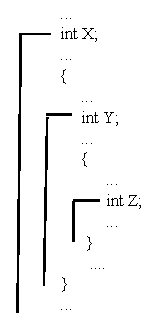
\includegraphics[width=9cm,height=6cm]{images/scope1.eps}}
\setlength{\unitlength}{1cm}
\begin{picture}(12,5)
\codefont{
\put(0.2,4.5){int main()\{}
\put(0.5,4.0){int x = 7;}
\put(0.5,3.5){int y;}
\put(0.5,3.0){\emph{y = foo(x);}}
\put(0.5,2.5){...}
\put(0.2,1.0){\}}
}

\put(4.2,4.3){The \emph{value} of \codefont{x} is copied into \codefont{z}}
\put(4.2,3.8){when the function is called.}
\linethickness{0.3mm}
\ifcolor\color{\mycolor}{
\put(4.1,3.6){\vector(1,0){5.5}}
\put(3.5,3.3){\line(1,0){0.5}}
\put(3.5,3.8){\line(1,0){0.5}}
\put(3.5,3.3){\line(0,1){0.5}}
\put(4.0,3.3){\line(0,1){0.5}}


\put(3.5,2.3){\line(1,0){0.5}}
\put(3.5,2.8){\line(1,0){0.5}}
\put(3.5,2.3){\line(0,1){0.5}}
\put(4.0,2.3){\line(0,1){0.5}}

\put(10,3.3){\line(1,0){0.5}}
\put(10,3.8){\line(1,0){0.5}}
\put(10,3.3){\line(0,1){0.5}}
\put(10.5,3.3){\line(0,1){0.5}}

\put(10,2.3){\line(1,0){0.5}}
\put(10,2.8){\line(1,0){0.5}}
\put(10,2.3){\line(0,1){0.5}}
\put(10.5,2.3){\line(0,1){0.5}}


\put(9.8,2.7){\vector(-1,0){5.5}}
\ifcolor}
\color{Black}{
\put(9.9,2.4){12}
\put(10.1,3.4){7}
\put(9.9,3.9){\codefont{z}}
\put(9.9,2.9){\codefont{a}}
\put(3.6,3.4){7}
\put(3.4,3.9){\codefont{x}}
\put(3.4,2.4){12}
\put(3.4,2.9){\codefont{y}}\put(0,0){\large\textbf{main() and its variables}}

%\put(7,0){\line(0,1){5}}

% ----------------  func
\codefont{
\put(11.5,4.5){\emph{int foo(int z)}\{}
\put(11.8,4.0){int a;}
\put(11.8,3.5){a = z + 5;}
\put(11.8,3.0){...}
\put(11.8,1.5){return a;}
\put(11.5,1.0){\}}
}


\put(4.4,2.3){The \emph{value} of \codefont{a} is copied into \codefont{y}}
\put(4.4,1.8){when the function returns.}

\put(10.5,0){\large{\textbf{foo() and its variables}}}
}
\end{picture}
\caption{When a function is called, the value of the arguments are copied into the function's parameters.  When a function returns, the return value (if any) should be copied into a variable in the calling function.}
\label{fig:arguments}
\end{figure}

Functions are defined as shown in Figure~\ref{fig:functions1}.
The return type of a function is the type (e.g., \codefont{int}) of value that the function returns.  If the function doesn't return a value, then the type is \emph{void}\index{void@{\cf{void}}}.  The function name is the name of the function.  Data may be passed to a function as arguments and stored in the function's parameters.  An ``answer'' can be returned via the return command.  A return statement can return a value (e.g., \codefont{return 7}) or a variable (e.g., \codefont{return X}), so long as the type of the returned value matches the return type in the function definition.  For example, on lines 8 and 9b, the return type of the function \codefont{get\_value()} is \codefont{double} (a new type) and the returned variable \codefont{temp\_value} has type \emph{\cf{double}} (declared on line 10b) and returned on line 13b.

The calculator program has four functions: \codefont{main()}\footnote{We have already seen that as a function, \codefont{main()} can return a value.  It turns out that \codefont{main()} can also receive arguments.  This is discussed in Interlude 6.}, \codefont{print\_menu()}, \codefont{get\_value()}, and \codefont{divide()}.  The \codefont{main()} function was already examined in Chapter 1.  The other functions are described in the following sections.

Functions must be called with the correct number and types of arguments.  When a program is compiled, the compiler checks whether functions are called with the correct number of arguments, which is only possible if it knows what the arguments should be; that is, it knows the functions' parameters.  This is the role of the \emph{prototypes}\index{prototype}.  Each of the three defined functions (\codefont{print\_menu()}, \codefont{get\_value()}, and \codefont{divide()}), has a prototype (on lines 7, 8, and 9, respectively).  A prototype defines the format of a function so the compiler can check that the function is being called properly.  For example, the prototype on line 9 tells the compiler that \codefont{divide()} must be called with two values or variables of type \cf{double} and should return a value of type \cf{double}.  If the \codefont{divide()} function is called with the wrong number or type of arguments, the compiler reports an error.  Another term for prototype is function \emph{declaration} because they are similar to a variable's declaration.  

\mysubsubsection{Pass-by-Value}\index{pass-by-value}\index{functions!pass-by-value}\index{arguments!pass-by-value}

An important aspect of parameters in C++ is that by default, they are \emph{pass-by-value}.  This means that the value of the argument is copied into the parameter in the function -- the function has access to the value, but \emph{not} the original ``box'' that the variable was stored in (see Figure~\ref{fig:arguments}).  Thus, any changes made to the value in the function are lost when the function exits, unless the new value is explicitly returned as part of the return statement.

For example, in the Calculator program on line 12b of the \codefont{get\_value()} function, the user's input is stored in the variable \codefont{temp\_value}.  However, to get that value back to the \codefont{main()}, the value must be returned (line 13b)  and stored in a new variable; for example, on line 23 where the returned value is stored in \codefont{operand1}.

An alternative approach to pass-by-value parameters is to use pass-by-reference parameters, which are discussed in Chapters 5 and 6.

\begin{figure}
%\centerline{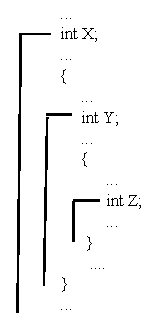
\includegraphics[width=9cm,height=6cm]{images/scope1.eps}}
\setlength{\unitlength}{1cm}
\begin{picture}(10,4)

\linethickness{0.3mm}
\put(2,2.5){\codefont{double divide(double dividend, double divisor)\{}}
\put(2.5,2){\codefont{code ...}}
\put(2.5,1.5){\codefont{return answer;}}
\put(2,1){\codefont{\}}}

\put(0.5,3.5){return type}
\color{\mycolor}{
\put(1.7,3.4){\vector(1,-1){0.5}}
\put(3.0,3.9){\vector(1,-2){0.55}}
\put(5.8,3.4){\vector(-1,-1){0.5}}
\put(7.9,3.4){\vector(1,-1){0.5}}
\put(7.4,2){\vector(-1,1){0.4}}
\put(8.9,2){\vector(2,1){0.8}}
\put(12.2,3.1){\vector(-2,-1){0.6}}
\put(2.85,0.7){\vector(-2,1){0.6}}
\put(5.95,1.2){\vector(-2,1){0.6}}
}

\color{black}{
\put(2,4){function name}
\put(5,3.5){parameter types}
\put(7.1,1.7){parameters}
\put(6.0,1.1){return statement}
\put(9.0,3.3){beginning \} starts the function}
\put(3,0.5){closing \} ends the function}
}

\end{picture}
\caption{The parts of a function definition. A function can have zero or more parameters, which may have different types.  A function has a return type (or \emph{void} if the function doesn't return a value).  A function may have several return statements in its code, but the first one reached returns a value and ends the function.}
\label{fig:functions1}
\end{figure}

\subsection{Functions with the Same Name}

In C++, it is legal to have two, or more, functions with the same name \emph{if they have different numbers or types of parameters}.  For example, two different divide functions could be defined with the following prototypes:\\
\codefont{
double divide(double dividend, double divisor);\\
double divide(double dividend, double divisor, double x);\\
}
The different type or number of parameters is necessary so that the compiler knows which function to call; that is, the function whose parameters match the arguments.  So, in the previous example, the command \codefont{divide(6.0, 2.5)} would be matched to the first version of the function and the command \codefont{divide(6.0, 2.5, 1.8)} would be matched to the second version of the function.


\subsection{Real Number Types}\index{double@{\cf{double}}}\index{type!double@{\cf{double}}}

The \codefont{double} type is used to store real numbers.  The term \cf{double} is derived from \emph{double precision}, which stands for a number that uses twice as much memory as a ``standard'' variable, which allows it to store more decimal places -- that is, to be more precise\index{double@{\cf{double}}}\index{type!double@{\cf{double}}}.  With the increase in the amount of memory that is cheaply available, \cf{double} has become the most common type for storing decimals in C++. Variables of type \cf{double} are stored in memory using scientific notation, with a fixed amount of memory reserved for the mantissa (or precision number) and a fixed amount of memory reserved for the exponent.  Because scientific notation is used, a double can represent a very large or very small number, but the precision is somewhat limited compared to the absolute size of the number (see Section~\ref{appendix:types} of Appendix A).  

\subsection{Conversions and Casts}\index{cast}\index{conversion}\index{promotion}

It is often necessary to convert the type of a value; for example, changing an \codefont{integer} into a \codefont{double} or vice versa.  This is most common in mathematical expressions that involve variables of more than one type.   For example, the code:\\
\cf{
int x = 11;\\
double var = 4;\\
var = x/var;\\
}
division is performed with an \cf{integer} (\cf{x}) and a \cf{double} (\cf{var}) and the result is stored in a \cf{double}.  What should the variable \cf{var} store?

C++ has implicit rules for converting between types (also known as casting).  There are two rules that are particularly important.  First, when operating on two different types C++ \emph{promotes} the lower precision value to the higher precision value.  So, in the previous example when \cf{x} is divided by \cf{var}, the value held by \cf{x} (e.g., 11) is temporarily promoted to a double (think of it as 11.0).  Thus, the division is treated as \cf{11.0/4.0} and the answer is 2.75, which is stored in \cf{var}.

Second, if a decimal value has to be stored in an integer type the value is \emph{truncated} (not rounded).  For example, if the previous code were changed to:\\
\cf{
int x = 11;\\
double var = 4;\\
x = x/var; // now the answer is stored in x\\
}
the division is the same (\cf{11.0/4.0 = 2.75}), but the answer has to be ``squished'' in to an integer (\cf{x}).  In this case C++ truncates the answer and \cf{x} ends up storing the value 2 (\emph{not} 3).

In understanding how C++ applies the first rule (when operating on two different types \emph{promote} the lower precision type to the higher precision type) it is important to realize that it is applied for each operation \emph{independently}.  For example, in the code:\\
\cf{
int x = 11;\\
double var = 4.5;\\
var = (x/12) * (x + var + 1000); \\
}
the variable \cf{var} will store the answer \emph{zero}.  The first operation C++ performs is \cf{x/12}, both \cf{x} and 12 are integers, so neither is promoted and the answer for that part of the calculation is truncated to zero, which leads to the final answer of zero.  A completely different answer is obtained simply by changing the calculation to:\\
\cf{var = (x/12.0) * (x + var + 1000); }\\
now the division (\cf{x/12.0}) is performed on an \cf{integer} (\cf{x}) and a \cf{double} (\cf{12.0}), the \cf{integer} is promoted to a \cf{double}, and that part of the expression is not truncated.  An alternative solution is to write the code as:\\
\cf{var = (double(x)/12) * (x + var + 1000); }\\
this tells C++ to treat the value in \cf{x} as a \cf{double} just for that part of the calculation.  (The variable \cf{x} is explicitly \emph{cast} as a \cf{double}.) In this case the 12 is also promoted to a double and the answer is not truncated.\footnote{Other languages treat mixed expressions with mixed types very differently.  For example, many languages \emph{require} explicit casting whenever two different types are combined. and will produce a compiler error otherwise.}

In creating expressions with mixed types it is very important to pay careful attention to how casting will work.  C++'s built-in rules for implicitly converting types, are only a guess at what the programmer intended and often give unexpected and undesired results.  Careful use of decimals and explicit casts will avoid a lot of program errors.  In addition, on many C++ compilers it is possible to increase the \emph{strictness}, which will cause the compiler to produce a warning whenever it identifies a piece of code that requires converting from a higher precision type to a lower precision type.  This can also be useful in avoiding difficult to identify errors causes by unexpected truncation in mathematical expressions with mixed types.


%-----------------------------------------------

\section{Analysis of the Code}

The general structure of the calculator program is relatively straight forward.  It consists of a main loop, similar to NIM, which allows the user to perform different calculations without having to restart the program.  Within this loop is a menu structure that allows the user to select which operation to perform.  A switch statement is used to process the user's choice.  Additional functions, like \codefont{get\_value()}, simplify the code for each of the user choices.
%General description of the code

\mysubsubsection{Lines 1-3: Comment Block}
As with the NIM program, these lines are a comment block briefly describing what the program does.

\mysubsubsection{Lines 4-5: \#includes}
As with the NIM program, these lines are preprocessor commands that include necessary libraries.

\mysubsubsection{Lines 7-9: Function Prototypes}

These are the prototypes for the functions \codefont{print\_menu()}, \codefont{get\_value()}, and \codefont{divide()}.  The prototypes declare a function's name, parameters, and return type. 

An alternative approach is to write the entire function definition before the \codefont{main()} function.  In this case, the prototype is not required because the compiler has access to the entire function definition right from the start.  There are two problems with this approach.  First, it's not considered good programming practice.  Second, if the code has two functions that call each other (e.g., function \codefont{A()} calls function \codefont{B()} and function \codefont{B()} calls function \codefont{A()}) then it is necessary to have prototypes.  Otherwise, the compiler will give an error in whichever function comes first in the code, because the compiler will not have seen the other function's definition.

A third approach, discussed in Chapter 7, is to place the function code in a separate, user-defined library.  This is useful when the functions are general-purpose and may be used in many different programs. 

\mysubsubsection{Lines 1b-22b: Function Definitions}

The code for the functions is presented in Listing~\ref{listing:calcFunctions}.

The \codefont{print\_menu()} function (lines 16b-22b) is the simplest of the functions.  It doesn't take any arguments; that is, no data is passed to the function, and it doesn't return a value.  So, on line 16b, where \codefont{print\_menu()} begins, the return type is \emph{void} and there is nothing inside the parentheses.  The function consists of a series of output commands.  When the function is called, it generates some output and, when it reaches the function's last \} on line 22b, it returns to the place in the code where it was originally called from.  The output commands could have been put in the main function, but by making a separate function, the program is divided into more readable blocks.

The next simplest function is \codefont{get\_value()}, defined on lines 9b-14b.  It also doesn't take any arguments, but it does return a value (of type \codefont{double}).  Thus, on both lines 8 and 9b, the return type for the \codefont{get\_value()} function is \codefont{double}.  The function itself creates a variable called \codefont{temp\_value} (line 10b), gets a value from the user that is stored in \codefont{temp\_value} (line  12b), and then returns that value (line 13b).  

Thus, when the program gets to line 23 (or line 24, 28, or 29), it jumps to the \codefont{get\_value()} function that starts on line 9b.  The \codefont{get\_value()} function gets a value from the user (line 12b) and then returns it (line 13b).  Back on line 23, the returned value is stored in the variable \codefont{operand1} (or \codefont{operand2} on lines 24 and 29).  Notice that the names of the variables are different because two different ``boxes'' are involved: a box/variable called \codefont{temp\_value} in the function and a box/variable called \codefont{operand1} (or \codefont{operand2}) in main; only the \emph{value} that was stored in \codefont{temp\_value} is copied from the function to the variable in main.  

Note that in the \cf{main()} function, the \codefont{get\_value()} function is called in several places (lines 23, 24, 28, and 29).  This is one of the major advantages of a function -- instead of having to write the same piece of code over and over, it can be written once as a function and then called whenever it is needed.

\begin{wrapfigure}{R}{0.5\textwidth} \framebox[\linewidth][l]{\parbox{0.9\linewidth}{\codefont{Matching Arguments and Function Calls} \\
When a function is called, it is critical that it is passed the correct number and type of variables.  For example, whenever the divide function is called, it \emph{must} receive two values of type \cf{double}.  Thus, on line 30, where \codefont{divide()} is called, there must be two values or variables of type \cf{double} in the parentheses to match the two arguments on line 2b.  Mismatched arguments are a common error in programming.  
}}
\vspace{-0.5cm}
\end{wrapfigure}

The \codefont{divide()} function, lines 2b-7b, has both a return value and two parameters, all of which have the type \codefont{double}.  The two parameters are named \codefont{dividend} and \codefont{divisor}.  These variable names are not the same as are used when calling the function from \codefont{main()} (line 30).  The variables in the calling function (in this case, \codefont{main()}) and in the called function (in this case, \codefont{divide()}) are independent -- only the values are copied from the calling function to the called function. 

After receiving its arguments, the \codefont{divide()} function begins by checking whether the divisor is zero (line 3b).  If a C++ program tries to divide by zero, the results are unpredictable and the entire program may crash\index{divide by zero}.  Thus, it is important to make sure that the divisor is not zero before doing the division on line 6b.  If the divisor is \emph{not} zero, the program divides and returns the answer in one step.  However, if the divisor is zero, the program still has to return a value (that's the way the function is defined, it returns a \cf{double}), so as a temporary solution, it returns a zero (line 4b).

The \codefont{divide()} function has two return commands on lines 4b and 6b.  As soon as one of them is reached, the program \emph{returns} to where it was called from and none of the code after the return command gets executed.  

\mysubsubsection{Lines 11-12, 41: Main}

Lines 11-12, and 41 define the \codefont{main()} function.  The syntax of the \codefont{main()} function should now be a little clearer.  It takes no arguments (although this can be changed -- see Interlude 6), and it ends by returning a 0 on line 40.

\mysubsubsection{Lines 13-14: Variables}

Lines 13-14 declare the variables used in the \codefont{main()} function.  Note that, three variables (\codefont{operand1}, \codefont{operand2}, and \codefont{answer}) are declared simultaneously on line 13.  So long as the variables have the same type, they can be declared together.  

\mysubsubsection{Lines 15-39: The Calculator Loop}

Lines 15 and 39 define a \cf{do-while} loop similar to the one used in NIM in Chapter~\ref{ch:NIM}.  This loop allows the program to perform repeated computations until the user is done.  The termination condition for the loop, part of the \cf{while} command on line 39, is:\\
\codefont{choice != 0}\\
This is true so long as the value stored in the variable \codefont{choice} is \emph{not} equal to 0 (the character pair != stands for not equal).  Therefore, so long as the user's choice is not zero, the program will continue to loop, and when the user chooses 0, the loop ends.

\mysubsubsection{Line 16: Print Menu}

Line 16 calls the \codefont{print\_menu()} function.  The computer jumps to the beginning of that function and begins running the code within the function, which prints the menu options to the screen.  The function ends when when it reaches the closing \} on line 22b and the computer jumps back to line 16 where the function was called.

\mysubsubsection{Line 18: A Valid Choice}

Line 18 sets the value of the variable \codefont{valid\_choice} to 1.  As the comment (everything after the //) explains, a 1 means that the computer ``thinks'' the user has entered a valid menu option.  If this is not true, the value is changed to 0 later in the code.  On line 36, the value stored in \codefont{valid\_choice} is used to determine whether the answer should be printed.  If \codefont{valid\_choice} is 1, meaning the user made a valid choice from the menu options, the answer is printed.  If the value of \codefont{valid\_choice} is 0, meaning the user did not make a valid choice, the answer isn't printed.

\mysubsubsection{Lines 19-35: Switch Statement}\index{switch@{\cf{switch}}}

Line 19 is the beginning of a switch statement.  A \emph{switch} statement is a conditional statement like an if-else statement.  It is particularly useful when there are multiple, discrete options, as in a menu.   
%A switch statement takes an integer type as input and then jumps to the matching \emph{case}\index{case}.

The general format of a switch statement is:\\
\codefont{
switch(\emph{variable})\{\\
\hspace*{0.5cm}      case 1:\\
\hspace*{1.0cm}  \emph{code block 1}\\
\hspace*{1.0cm} break;\\
\hspace*{0.5cm}   case 2:\\
\hspace*{1.0cm}  \emph{code block 2}\\
\hspace*{1.0cm}   break;\\
\hspace*{0.5cm}    ...\\
\hspace*{0.5cm}    default:\\
\hspace*{1.0cm}  \emph{code block N}\\
\hspace*{1.0cm}   break;\\
\}\\
}
When the \codefont{switch} is reached, the value of \codefont{\emph{variable}} is checked and the program jumps to the matching \emph{case}\index{case@{\cf{case}}}.  For example, if the variable's value is 3, then the program jumps to case 3.  If there is no matching case, then the program jumps to the \emph{default}\index{default@{\cf{default}}} case.  Typically, the cases are positive and in order (1, 2 , 3, etc.) but any integer values in any order will work.\footnote{Switch statements can also use a variable of type \codefont{char}, which is short for \emph{character} and will be introduced in Chapter 5.} 

Each case ends with a \codefont{break}\index{break@{\cf{break}}} statement.  When the program reaches a break statement, it jumps to the end of the switch statement: the closing \}.  Without the break statement, the program will ``fall through'' the other cases and execute them as well.\footnote{Break statements can also be used to break out of loops or conditionals.  However, this is generally considered to be poor programming practice and should be avoided.}  For example, without breaks, if the variable had the value 2, the program would jump to case 2, but then it would continue to execute case 3, case 4, etc., all the way through the default case.  

The case statement can only have a single, fixed value.  Statements like:\\ \codefont{case <5:} and \codefont{case 4 to 10:} \\will \emph{not} work.  One approach that does work is to ``stack'' cases:\\
\codefont{
case 2:\\
case 3:\\
case 4:\\
\hspace*{0.5cm} \emph{code ...}\\
\hspace*{0.5cm} break;\\
}
This will result in the same code being applied to cases 2 through 4.

\mysubsubsection{Lines 20-21: Case 0}
If the user enters a 0 (for exit), the switch statement just executes a break and jumps to the end of the switch statement.  From there, the \cf{do-while} loop ends, because the variable \codefont{choice} has the value 0, which causes the main loop to end.  %Alternatively, the program could end immediately by putting \codefont{return 0;} on line 21.

\mysubsubsection{Lines 22-26: Case 1}
If the user enters a 1 (for addition), the program uses the \codefont{get\_value()} function twice to get two numbers from the user and stores them in the variables \codefont{operand1} and \codefont{operand2}.  Then it adds them and stores the result in the variable \codefont{answer} (line 25) to be printed later (line 37).  Finally, the break statement causes the program to jump to the end of the switch statement (line 35).

\mysubsubsection{Lines 27-31: Case 2}
If the user enters a 2 (for division), the program uses the \codefont{get\_value()} function twice to get two numbers from the user and stores them in the variables \codefont{operand1} and \codefont{operand2}.  Then it divides them using the divide function and stores  the result in the variable \codefont{answer} (line 30) to be printed later (line 37).  Finally, the break statement causes the program to jump to the end of the switch statement (line 35).

\mysubsubsection{Lines 32-34: Default}

If the user enters any value besides 0, 1, or 2, the program jumps to the \emph{default} case.  There, the variable \codefont{valid\_choice} is set to 0, for false, and the message \codefont{Invalid Choice} is printed to let the user know that he or she entered an invalid choice.  The variable \codefont{valid\_choice} is set to 0, which keeps the program from printing an answer when it reaches line 36. 

Including a default case is not required in C++, but it is a very good idea.  Even if you are sure that every possible case is covered without the default, including a default case that prints an error message makes debugging the code much easier if an unexpected case does occur.

\mysubsubsection{Lines 36-38: Print the Answer}

Line 36 uses an if statement to check whether the user entered a valid menu choice.  A common C++ trick is used in the condition in line 36.  Instead of comparing \codefont{valid\_choice} to 0 or to 1 the conditional in the if statement  is just the variable \codefont{valid\_choice}.  In C++, any zero value is considered false, and any nonzero value is considered true.  So, on line 36, if \codefont{valid\_choice} is 1, it is considered \emph{true} and the answer is printed.  If \codefont{valid\_choice} is 0, from line 33, then it is considered \emph{false} and the \codefont{cout} statement is skipped.

\subsection{Scope}\index{scope}

\begin{wrapfigure}{R}{0.5\textwidth} \framebox[\linewidth][l]{\parbox{0.9\linewidth}{\codefont{Scope, Variable Names, and Team Projects} \\
Most commercial software products are written in separate blocks by members of a large team.  Scope separates variables in different blocks of code.  For example, the variable \codefont{X} in one block of code is independent of any other variables called \codefont{X} declared in other blocks of code.  Thus, in a large programming project any programmer is free to select their own variable names without having to worry about them conflicting with variables in another part of the program -- as long as the scope of the variables don't overlap.
}}
\vspace{-0.5cm}
\end{wrapfigure}

In this program, there are variables in \codefont{main()} and variables in most of the functions.  Some of these variables may have the same name, but they don't represent the same ``box.''  If they did represent the same ``box'' it would become very confusing, especially in  large programs written by teams of programmers.  No one would ever know which variables had already been created elsewhere in the code or where else in the code the values for ``their'' variables might be changed.

\emph{Scope} solves this problem by limiting the regions of code in which a particular variable is valid and can be used.  The basic rule for the scope of a variable is simple: a variable's scope extends from where the variable is declared to the right curly brace \} ending the block of code that the variable is declared in (see Figure~\ref{fig:scope1}).

\begin{figure}
%\centerline{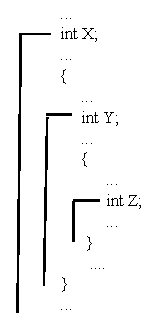
\includegraphics[width=9cm,height=6cm]{images/scope1.eps}}
\setlength{\unitlength}{1cm}
\begin{picture}(8,7)
%\codefont{
%\linethickness{0.3mm}

\put(1.5,6.5){int main()\{}
\put(2,6){\emph{int \codefont{X};}}


\put(2,5.5){\{}
\put(2.5,5){code ...}
\put(2.5,4.5){\emph{int \codefont{Y};}}
\put(2.5,4){code ...}
\put(2.5,3.5){\{}
\put(3,3){code ...}
\put(3,2.5){\emph{int \codefont{Z};}}

\put(3,2){code ...}
\put(2.5,1.5){\}}
\put(2.5,1){code ...}
\put(2,0.5){\}}

\put(1.5,0){\}}

% ---- func

\put(6.5,6.5){int func(int X)\{}
\put(7,6){\emph{int \codefont{Y};}}
\put(7,5.5){code ...}
\put(6.5,3){\}}

\ifcolor\color{\mycolor}{
\put(0.88,5.1){\codefont{X}}
\put(1.5,3.9){\codefont{Y}}
\put(2.05,2.1){\codefont{Z}}
\put(6.05,5.9){\codefont{X}}
\put(6.55,5.2){\codefont{Y}}

\put(1.3,6.2){\vector(0,-1){5.7}}
\put(1.8,4.7){\vector(0,-1){3.7}}
\put(2.3,2.7){\vector(0,-1){1.2}}

\put(6.3,6.6){\vector(0,-1){3.2}}
\put(6.8,6.2){\vector(0,-1){2.8}}
\ifcolor}

\end{picture}
\caption{Illustration of scope.  The vertical lines mark the scope of each of the variables \codefont{X}, \codefont{Y}, and \codefont{Z} (including second variables \cf{X} and \cf{Y} in the function).  Scope extends from the where the variable was declared to the closing bracket \} marking the end of that block of code.  Note that scope includes any nested blocks, for example, \codefont{Y}'s scope includes the nested set of brackets \{\} where \codefont{Z} is declared, and \codefont{X}'s scope includes the scope of both \codefont{Y} and \codefont{Z}.   Any reference to a variable outside of its scope will result in a compiler error or warning.  The variables \codefont{X} and \codefont{Y} in the function \codefont{func()} have their own scope and are separate from the variables of the same name in \codefont{main()}. }
\label{fig:scope1}
\end{figure}

Any reference to a variable outside that variable's scope is an error that will be caught and reported by the compiler.  One way to think of this is that when a program reaches the end of a variable's scope, the ``box'' corresponding to that variable is destroyed.\footnote{Actually, when a variable reaches the end of its scope, the variable is no longer usable, but the value it stored is often left in memory, where it's hard, but not impossible, to access.  This can lead to security problems if the value needs to be secure.  Thus, in sensitive programs, it's a good idea to ``zero out'' a variable's value before leaving its scope.}  Another variable of the same name could be declared somewhere else in the code, but this would be a separate box, with no connections to the original variable of the same name.

Scope is particularly important in using functions.  The scope of a variable only extends to the function it was declared in.  For example, in the calculator program, there is a variable called \codefont{answer} declared in \codefont{main()} on line 13.  This variable cannot be used in any of the functions.  The value of \codefont{answer} cannot be set, and its value cannot be accessed, from any of the functions.  

To test the scope of the variable \codefont{answer}, try the following.  Replace line 6b of the program with the following new line:\\
\codefont{answer = dividend/divisor;}\\
This may appear to set \codefont{answer} to the correct value so it can be printed in \codefont{main()}.  Instead a compiler error is generated because the scope of  \codefont{answer} does not extend to the function \codefont{divide()}.  That's why the function \codefont{divide()} has to return the correct value, so that it can be stored in the variable \codefont{answer} on line 30.

Whenever a function is created it's important to think about what data is being sent to the function (the arguments) and what data, if any, the function is returning.  Carefully planning the data flow for a function before beginning to program it will avoid many potential errors.

% box globals
\vspace{+0.25cm}
{\color{\mycolor}\noindent\hrulefill}
\section{Exercises: Modifying the Program}
By now, you should have a general idea of how the program works.  However, there are many changes and improvements that can be made.  The suggested modifications begin with a few simple changes before moving on to more complex and more interesting changes.  Not all of the new code will be given, in many places, only suggestions about how to proceed are provided.

\mysubsubsection{Exercise 1: Modifying the Output}

Add some initial output printing information about the program: the name of the author (you), the date it was created, and a brief explanation of its functionality.  This is done with one or more \codefont{cout} statements that print the desired information near the beginning of the program.  

\mysubsubsection{Exercise 2: The Final Answer}
Fix the minor, but annoying, problem that when the user exits, the program reprints the last answer.  
The best way to fix this flaw is to use the existing conditional on line 36.  One option is to expand the condition so that it prints the answer only if the user made a valid choice and didn't choose to exit, making the condition\\
\codefont{valid\_choice \&\& (choice != 0)}\\
Alternatively, case 0 could be modified to make \codefont{valid\_choice} 0, which would also keep the answer from being printed.  Note that both of these solutions have the advantage of using the conditional that's already part of the program rather than having to add a lot of new code.

\mysubsubsection{Exercise 3: Printing Answers and Problems}
Currently, the program just prints the answer to each of the user's problems.  Change the output so that the program prints the whole problem as a mathematical expression.  For example, if the user asks for the sum of $4.5$ and $1.3$, the program currently prints:\\
\codefont{answer = 5.8}\\
whereas it could print:\\
\codefont{4.5 + 1.3 = 5.8}\\
Changing line 37 to something like:\\
\codefont{cout << operand1 << "???" << operand2 << " = " << answer << endl;}\\
works except for the ??? part.  What should go there?  The problem is that the program has ``forgotten'' which operation the user picked.  One approach is to replace line 37 with another switch statement based on the \codefont{choice} variable, such as\\
\codefont{
switch(choice)\{\\
\hspace*{0.5cm}case 1: \\
 \hspace*{1.0cm}         cout $<<$ operand1 $<<$ "+" $<<$ operand2 $<<$ " = " $<<$ answer $<<$ endl;\\
   \hspace*{1.0cm}       break;\\
\hspace*{0.5cm}     case 2:\\
  \hspace*{1.0cm}           cout $<<$ operand1 $<<$ "/" << operand2 $<<$ " = " $<<$ answer $<<$ endl;\\
 \hspace*{1.0cm}            break;\\
...\\
\}\\
}
Then for each choice, the program prints the correct output (the default case wouldn't print anything because it's an invalid choice).

However, the code already contains a switch statement very similar to this one.  Reusing the existing switch statement will shorten the program and adding more options will only require changing one switch statement, not two.  To use the existing switch statement, the first part of the output is printed within the switch statement and the answer is still printed on line 37.  For example, an extra line would be added between lines 25 and 26:\\
\codefont{cout << operand1 << "+" << operand2 << " = ";}\\
and a similar line would be added between lines 30 and 31:\\
\codefont{cout << operand1 << "/" << operand2 << " = ";}\\
Note that these have the correct operator, but they don't print the answer yet (although they could).  Then line 37 would be changed to just\\
\codefont{
cout << answer << endl;}\\
This way, the mathematical expression is printed from one line and the answer is printed from a very different line, but because of the way the spacing is used, it looks like one expression in the output.
         
\mysubsubsection{Exercise 4: More Functionality -- Subtraction}

Of course, the biggest drawback to this calculator is that it can only do two things: addition and division.  However, the program was designed to make it (fairly) easy to add other functions.  Add an option that allows the user to perform subtraction.  

This requires two changes.
First, subtraction needs to be added as an option in the \codefont{print\_menu()} function.  This just requires adding a line like\\
\codefont{cout << "Subtract (3)" << endl;}\\
around line 19b.

Second, a new case (case 3) needs to be added to the switch statement that starts on line 19.  Copy the addition case (lines 22-26), change the case number from 1 to 3, and the operation from addition to subtraction.  It is a good idea to rearrange and renumber the menu options so that the operations are in a more natural order, making sure that the choices in the menu match up with the cases in the switch statement.

\mysubsubsection{Exercise 5: More Functionality -- Minimum}

\begin{wrapfigure}{R}{0.5\textwidth} \framebox[\linewidth][l]{\parbox{0.95\linewidth}{\codefont{The cmath Library}\index{libraries!cmath@{\cf{cmath}}}\index{cmath@{\cf{cmath}}} \\
In addition to the mathematical operators already described and listed in Section~\ref{appendix:operators} of Appendix A there is a C++ library called \codefont{cmath} that defines many additional mathematical functions: sine, cosine, square root, etc.  These are actual functions; for example to calculate the sine of a variable called \codefont{angle}, the command would be:
\codefont{sin(angle);}  To include the library, add the line:
\codefont{\#include$<$cmath$>$}
with the other include statements.
Using the math library, the calculator program can be expanded to include many more functions.  The full details of the \codefont{cmath} library can be found online.
}}
\vspace{-0.0cm}
\end{wrapfigure}

Add a minimum operation that prints the minimum of two values entered by the user.  The minimum should be calculated by calling a function (like the current \codefont{divide()} function) that will need to be written as well.  (In general, a function should be used when more than a few lines of code are necessary to perform the calculation.)

The first steps are to add the new option in the \codefont{print\_menu()} function and to add a new case to the switch statement.  The new case should call a function called \codefont{minimum()}.  The new case should be similar to the divide case (lines 27-31), but the case number needs to be changed and instead of calling  \codefont{divide(operand1,operand2)}, the new case should call \codefont{minimum(operand1,operand2)}.  

Next, the \codefont{minimum()} function needs to be written.  Start by copying the divide function (lines 2b-7b).  Name the new function \codefont{minimum}.  The parameters (\codefont{dividend} and \codefont{divisor}) should be renamed to be more appropriate to the function.  The if-else statement (lines 3b-6b of the original function) need to be rewritten to return the minimum value.  The resulting function could look like\\
\codefont{
double minimum(double value1, double value2)\{\\
\hspace*{0.5cm} if(value1 < value2)\\
\hspace*{1cm} return value1;\\
 \hspace*{0.5cm} else\\
\hspace*{1.0cm} return value2;\\
\}\\
}
where, in this case, the new parameters are \codefont{value1} and \codefont{value2}, but they could be anything. 

Finally, a new prototype needs to be added so the compiler can check that the function is being used properly.  The prototype needs to be listed with the other prototypes somewhere between lines 7 and 9.  It should be:\\
\codefont{double minimum(double, double);}\\
Note that the prototype specifies the function name, number, and type of the parameters, as well as the return type.  

Now the \codefont{minimum()} function should be working. Run the program and choose the minimum option to test whether it works correctly.  Remember to check what happens if the user enters two values that are identical.  It's good practice to try to figure out what will happen by looking at the code before testing the results.

\mysubsubsection{Exercise 6: Absolute Value}

So far, all of the operators discussed (add, subtract, multiply, divide, and minimum) have had exactly two operands.  This is not a requirement.  A different operation might need one operand or three or more operands.  Note  that if a function requires more than two operands, additional variables (\codefont{operand3}, \codefont{operand4}, etc.) need to be declared on line 13.

Add an absolute value operation (an option that returns the absolute value of a number) to the calculator.  Because it calculates the absolute value of only one number, the \codefont{get\_value()} function only needs to be called once.  

\mysubsubsection{Exercise 7: Cartesian Distances}

Create an option that calculates the distance between two points in a Cartesian plane.  This option needs four values: the $x$ and $y$ value for each of the two points.  Once the four values are input by the user, write a new function that will accept the four values as arguments and calculate and return the distance between them.

%Functions calling other functions

\section{Problems}

The potential for extending the calculator program should now be clear.  Additionally, the basic framework, particularly the menu, can be used as the basis for many other programs.  The following problems explore these possibilities.

\begin{enumerate}[{\bf 1.}]
\item {\bf More complex operations} \\
Use the \codefont{rand()} function to create an option to generate random numbers, with one input from the user to determine the maximum random number.  (Review Chapter~\ref{ch:NIM} to see how to use the modulus operator to control the range of random numbers.)  

\item {\bf Customized calculator} \\
Customize the program for a particular application domain, such as geometry, chemistry, or physics.  Add at least three new calculations that are specifically designed for the new application.  For example, if the new calculator is designed for geometry applications add options for calculation areas, perimeters, etc.  Make sure the menu options are clear and that the program begins with some (brief) output explaining the calculator's purpose.
  
\item {\bf Reusing answers}\\
 Currently the calculator can perform only one calculation at a time.  Change the program to allow the user to use the previous answer directly as input for the next calculation without having to retype the answer.  For example, if the user adds two numbers, the sum can be used directly in the next calculation without reentering it.   Write the code so that after the program calculates an answer, it asks the user whether he or she wants to reuse that value and, if the user answers yes, \codefont{operand1} is set equal to the answer (instead of requesting a new \cf{operand1}) for use in the next calculation.  

\item {\bf Unlimited inputs}\\
 For some operations, it's not known in advance how many values the user wants to input.  For example, in an averaging operation, the user may want to average any number of values.  Create an \codefont{average()} function, like the \codefont{divide()} function, that has its own loop within the function for entering values.  The user should enter values one at a time, and after each value, the program asks whether the user wants to enter another value.  The program should keep a running sum of the values and the number of values entered to know what to divide by when the user stops entering values.

\item {\bf Menus in NIM}\\
Rewrite the NIM program so that users are given a menu of possible moves.  In the basic NIM game the options should be to remove one, two, or three objects.  The menu should not give illegal options, for example having the option to remove three objects when there are only two objects left.\\
{\bf Challenge:} Using the rules for making the computer play NIM intelligently (Exercise 6 of Chapter 3) have the program give the user hints as part of the menu options. 

\item {\bf Functions in NIM}\\
Rewrite the NIM program to use functions.  Create at least the two functions.  The first function should choose the computer's random move; the function should take the number of remaining objects as an argument and return a legal move.  The second function should allow the player to select their move; the function should take the number of remaining objects as an argument and only return a legal move.  

\item {\bf A Roulette game} - The basic calculator framework can be reused for other purposes.  Create a Roulette game in which the menu items correspond to potential bets: red, even, specific numbers, etc.  After the user has picked a bet, the program uses the \cf{rand()} to determine the outcome and reports whether the user won or lost.  \\
{\bf Challenge:} Allow the user to choose how much to bet and have the program keep track of the user's current bankroll (similar to the way the NIM game kept track of the objects remaining).

\item {\bf A sports strategy game} \\
Create a sports strategy game, where the menu helps the user pick a move (e.g., run or pass in a football game, or jab, hook, or block in a boxing game), then the computer picks a random countermove, and the outcome is based on the opposing moves.\\
{\bf Challenge:} Add a random factor to the outcomes.  For example, if the the user chooses to pass and the computer chooses to blitz (in a football game) it may be very likely that the user will lose a little yardage, but there's a small chance that they will gain a lot yardage.
\end{enumerate}

\addtocounter{interlude}{1}
\setcounter{section}{0}
\setcounter{figure}{0}

\interlude{Structures}
%\addtocounter{chapter}{-1}
%\addtocounter{chapter}{1}

The next chapter introduces classes, which are an extended data structure.  A class combines data and functions that act on that data in one compound definition.  Classes are the foundational data structure of C++ and other object oriented languages.
However, the C programming language does not support classes, any program that depends on or uses classes cannot be a C program.  
Instead of classes C has a precursor to classes known as a \emph{structure}\index{structure} that is defined using the keyword \codefont{struct}\index{struct}.  C structures allow a programmer to group multiple data types into one compound data type.  They are commonly used in ``pure'' C programs, such as on microcontrollers, and are useful for simple data structures even in C++.

The basic format of a structure definition is:\\
\cf{
struct fraction\{\\
\hspace*{0.5cm} int numerator;\\
\hspace*{0.5cm} int denominator;\\
\}; \\}
This creates a new, compound type called \cf{struct fraction} that contains two \cf{ints}.

However, programmers find using the name \cf{struct fraction} awkward and so most structure definitions are actually written like:\\
\cf{
\textcolor{\mycolor}{typedef} struct fraction\{\\
\hspace*{0.5cm} int numerator;\\
\hspace*{0.5cm} int denominator;\\
\} \textcolor{\mycolor}{fraction}; \\}
Note the keyword \cf{typedef} at the beginning and the extra \cf{fraction} at the end of the structure declaration.  This redefines the type \cf{struct fraction} with the new name \cf{fraction}.\footnote{The \cf{typedef} command can be used to rename any type, for example \cf{typedef int bob;} renames the type \cf{int} as \cf{bob}.  However, there are only a few places that \cf{typedef} is frequently used, dropping the \cf{struct} from structure names is one of them.}

Now there is a \cf{fraction} type:\\
\cf{fraction f1, x, my\_fraction;}\\
declares three new variables of type \cf{fraction}.

Each of these new variables is a compound variable containing two integers.  To access the data the \emph{dot notation} is used.  For example, the commands:\\
\cf{f1.numerator = 1;\\
f1.denominator = 2;\\
}
makes the variable \cf{f1} effectively store the number 1/2.  

Similarly, printing a structure requires printing each piece of data explicitly.  for example the command: \\
\cf{
cout $<<$ f1.numerator $<<$ "/" $<<$ f1.denominator;
}\\
will print \emph{1/2}.


Functions can be written that both accept structures as arguments and return structures.  For example:\\
\codefont{fraction add(fraction, fraction)}\\
Defines a function called \cf{add()} that takes two \cf{fraction} structures as arguments and returns a \cf{fraction} structure.  Presumably, the function adds the two fractions together, but that is determined by how the function is coded.

Like most programming constructs, structures can be nested, can contain other data types, and can contain a mixture of types.  For example, in program for a fantasy game the programmer might create a structure for holding data about a player's character:\\
\cf{
typedef struct character\{\\
\hspace*{0.5cm} char[100] name;  \hspace*{1.3cm}  // character's name\\
\hspace*{0.5cm} int maxhealth;     \hspace*{1.4cm}  // maximum health\\
\hspace*{0.5cm} int currenthealth; \hspace*{0.55cm}  // current health\\
\hspace*{0.5cm} weapon currentweapon;\hspace*{0.1cm} // another structure holding weapon information\\
\hspace*{0.5cm} float armorvalue; \hspace*{0.85cm}// current armor value \\
\} character;\\
}
Now all of the information about a player's character can be stored in one variable.

Careful use of structures can greatly simplify a complex program by grouping data together.  For example, if you find yourself creating multiple functions that all have the same long parameter list it's may be a good idea to create a single structure to hold all of the data.  Then the functions can be rewritten to have one a single parameter whose type is the new structure. 





%\addtocounter{chapter}{1}
\setcounter{section}{0}
\setcounter{figure}{0}
%********** Chapter 4 **********
\chapter{Electronic Pet}\index{Electronic Pet}\index{projects!Electronic Pet}\label{ch:pet}

\section{Introduction}

This chapter introduces the third project: the Electronic Pet.  The Electronic Pet program is similar to Tamagotchis, little electronic toy ``pets'' that have buttons to feed them, play with them, etc.  As with the previous projects, the initial version is limited, a pet can only be named, fed, and played with.  However, the structure of the program is flexible, making it relatively simple to add more features to the pet.  

This project reviews the topics covered in Chapters 2 and 3 and introduces several new elements of programming:
\begin{tight_itemize}
\item Classes\index{classes}, including:
\begin{tight_itemize}
\item Objects
\item Data members
\item Member functions (methods)
\item Constructors
\item Public and Private
\end{tight_itemize}
\item Strings\index{strings} 
\item Files\index{files}
\end{tight_itemize}

 A class is an abstract definition of a \emph{data structure}\index{data structure} that stores data and has functions that can act on the data.  Once a class is defined the programmer can create \emph{objects}\index{object} whose type is the same as the class.  For example, in this project, a \codefont{pet} class is defined and an object of type \cf{pet} is created.  A string is a new data type that can hold a ``string'' of characters.  It is useful for storing names, addresses, and similar types of data.  Files are used to store data when a program isn't running and to share data between programs.  In C++ the syntax for reading from and writing to files is similar to the syntax for reading from and writing to the keyboard and screen.

%\begin{itemize}
 % \item Classes
 % \item Data members
 % \item Function members
 % \item Constructors
 % \item Public versus private
 % \item Strings
%\end{itemize}

\section{The Program}

Listings~\ref{listing:electronic pet} and~\ref{listing:pet class} present the code for an electronic pet.  The program is divided into two sections.  Enter the code from \emph{both} Listings~\ref{listing:electronic pet} and~\ref{listing:pet class} as one long program, starting with the code in Listing~\ref{listing:electronic pet}.  (Again, do not enter the line numbers.)  As the program is entered, try to figure out what the statements do.  Many of them should be familiar, but others will be new.

\begin{minipage}{\textwidth}
\begin{lstlisting}[language=C++,numbers = left, xleftmargin=4.0ex, basicstyle=\small,emph={hunger, happy,name,pet1,choice,health_check},emphstyle = \color{\mycolor},
showstringspaces=false,
caption = {The \codefont{main()} and the declaration of the \cf{pet} class.},
label={listing:electronic pet}]
#include<iostream>
#include<string>
using namespace std;
// declaration of the pet class
class pet{
   private:
      int hunger;           // private data member
      int happy;            // private data member
      string name;          // private data member
   public:
      pet();                // constructor
      void play();          // public member function
      void feed();          // public member function
      void print();         // public member function
      int check_health();   // public member function
};
int main()
{
   pet pet1;
   int choice;
   int health_check;
   do{
       pet1.print();
       cout << "What would you like to do with your pet?\n";
       cout << " Play (1) \n Feed (2) \n Exit (0) \n";
       cin >> choice;
       switch(choice){
       case 1:
           pet1.play();
           break;
       case 2:
           pet1.feed();
           break;
      }
      health_check = pet1.check_health();
   }while(choice != 0 && health_check != 1);
   cin.ignore();
   cout << "Press enter to exit." << endl;
   cin.ignore();
   return 0;
}
\end{lstlisting}
\end{minipage}

Once the entire program has been entered, compile it.  As always, there may be some copying errors that need to be fixed.  Once the program compiles, run it and see what it does.  Be sure to test all of the menu options.  Are there any choices that produce unexpected output?  What happens if a nonexistent menu option is tried?  How do the user's choices affect a pet?

As with the previous projects, this program has some shortcomings.  Most notably, there are a limited number of options.  However, the program is written to make it easy to add to the pet's behavior, making it more fun and interesting to play with.  


\begin{minipage}{\textwidth}
\renewcommand*\thelstnumber{\the\value{lstnumber}b}
\begin{lstlisting}[language=C++,numbers = left,xleftmargin=4.0ex, basicstyle=\small, emph={hunger, happy,name,pet1,choice,health_check},emphstyle = \color{\mycolor},
showstringspaces=false,
caption = {Definition of the functions of the \cf{pet} class.},
label={listing:pet class}]
/* Constructor, creates a new pet with starting values. */
pet::pet(){
     hunger = 50;
     happy = 50;
     cout << "Pet's name? (One word) ";
     cin >> name;
}
/* Member function play(), allows playing with a pet. */
void pet::play(){
    int choice = 0;
    cout << "What should we play?\n";
    cout << " Fetch (1) \n Roll over (2) \n";
    cin >> choice;
    switch(choice){
    case(1):
         happy += 10;
         hunger += 5;
         break;
    case(2):
         happy += 5;
         hunger += 1;
         break;
    default:
         cout << "Not a valid choice." << endl;
   }
}
/* Member function feed(), allows the user to feed a pet. */
void pet::feed(){
    cout << "\nMMM, Yummy!\n";
    hunger -= 5;
}
/* Member function print(), prints information about a pet. */
void pet::print(){
    cout << "\nYour pet " << name << " is " << endl;
    cout << "Happy: " << happy << endl;
    cout << "Hungry: " << hunger << endl;
}
/* Member function check_health(), checks the health of a pet. */
int pet::check_health(){
    if(hunger >= 100){
         cout << "\nYour pet has starved.\n";
         return 1;
    }
    if(happy <= 0){
         cout << "\nYour pet has died of a broken heart.\n";
         return 1;
    }
    return 0;
}
\end{lstlisting}
\end{minipage}

\subsection{Classes}\index{classes}

 A \emph{class} is an abstract data structure consisting of \emph{data members}\index{data member}\index{classes!data member} and \emph{member functions}\index{function member}\index{classes!function member}, which are also called \emph{methods}\index{methods}\index{classes!methods}.  Data members are elements that store the data for an object\index{object}.  Member functions (or methods) are functions that act on that data.  A class can have multiple data members with different types and multiple member functions.  Figure~\ref{fig:class1} illustrates this idea for the \cf{pet} class used in this project, which has three data members and five member functions.  Once a class is defined, the programmer can create objects whose type is the class.  In this project, a \codefont{pet} class is defined, which allows objects of type \cf{pet} to be created.

A class is basically a programmer-defined, compound type.  Types, (e.g., \codefont{int} and \codefont{double}) allow the programmer to declare variables and to use the variable to store data.  For each type, there are associated operations (e.g., + and -) that can act on the variables.  
A class allows the programmer to declare objects, which can be thought of as variables whose type is a class and which can contain several pieces of data. For example, in this project, \codefont{pet1} is an object of type \codefont{pet} (see line 19), which stores several pieces of data regarding the pet (its hunger, happiness, and name).  Each class has associated functions, the member functions or methods, that can act on an object's data.    

A class definition is typically divided into two parts: the \emph{declaration} of the overall structure of the class (which is somewhat like a function prototype and contains prototypes for all of the class member functions) and the \emph{definitions} of the class member functions.  As with function definitions and prototypes, the class structure must be included before \cf{main()}\footnote{Or, more generally, it must be declared before it is used, just like variables and functions must be declared before they are used in the code.} and then the definitions of the functions (the actual function code) may be included later.  For example, in this project the structure of the \cf{pet} class is declared on lines 6-16, but the definitions of the member functions are defined on lines 1b-49b.\footnote{An alternative approach is to put the class in a separate file, which is discussed in later chapters.}

The data and functions of a class are accessed using \emph{dot notation}\index{dot notation}, which consists of the name of an object followed by a dot (.), followed by the name of the data member or member function to be accessed (see Figure~\ref{fig:memberfunctioncall}).  For example, line 23 shows the object named \codefont{pet1} accessing the \codefont{print()} member function of the \cf{pet} class using the statement:\\
\codefont{pet1.print()};\\
this makes the \codefont{pet1} object call its \codefont{print()} function, which is a member function of the class \codefont{pet}.

\subsection{Strings}\index{strings}\index{libraries!string@{\cf{string}}}

The term \emph{string} is a generic name for any data structure that holds a ``string'' of characters.  In C++ two types of strings are common, string objects and C-style strings.  In this chapter string objects are used, C-style strings are discussed in Interlude 4.   String objects are defined by the \cf{string} class, which is defined in the string library.  The string library is included on line 2 in the program.  Without line 2, the compiler and the program wouldn't know what a string was and any reference to a string in the code would generate a compiler error.  

A \cf{string} object holds a string of characters.  For example, in this program, the \codefont{name} object, which is of type \cf{string}, is used to store the name of the pet.  Strings can be obtained and printed using \codefont{cin} and \codefont{cout} just like other variables (see lines 6b and 34b).  The \cf{string} class contains dozens of member functions that can be used to manipulate, input, and output strings.  Only a few of the most useful functions are covered in this chapter.  Some of the other useful functions in the \cf{string} class are listed in Section~\ref{appendix:string} of Appendix A.

\section{Analysis  of the Code}

This program creates a single object of the \cf{pet} class; that is, it creates a ``pet.''  
%Each pet object has a \codefont{name}, a level of \codefont{happy}, and a level of \codefont{hunger}.  
A menu allows the user to select different ways to interact with the pet.  Each interaction has a different effect on the pet.  
The analysis of the code begins by analyzing the \codefont{pet} class.  Once it is clear how the class works, it's much easier to understand the rest of the program.
  
\mysubsubsection{Lines 5-16: The Pet Class Declaration}

Lines 5-16 declare the \cf{pet} class.  
%  As with function prototypes, a class must be declared before it can be used, typically before the \codefont{main()} function, and the actual code defining the functions of a class can come at the end of the program. 
Once the \cf{pet} class has been declared pet objects can be created (line 19).  Each pet object is a unique object that, like a variable, stores its own data.  Each pet object represents a unique, simulated pet that the user can interact with.  

Figure~\ref{fig:class1} illustrates the members of the \cf{pet} class, showing its three data members and five member functions in one structure.

Line 5 is the beginning of the definition of the \cf{pet} class.  (The rules for naming new classes are exactly the same as for other variables -- any valid variable name is a valid class name.)

Line 6 declares that the next few lines define \emph{private}\index{private} members of the \cf{pet} class.  The meaning of \emph{private} and \emph{public} will be discussed later in the chapter.  Each pet object has the following private data members:
\begin{tight_enumerate}
\item \codefont{hunger} - This is an integer that keeps track of the pet's current hunger level.  Feeding the pet decreases a pet's \codefont{hunger}, and playing with the pet increases it.  If a pet's \codefont{hunger} exceeds 99, the pet starves to death.
\item \codefont{happy} - This is an integer that keeps track of the pet's current happiness.  Playing with the pet increases its happiness.  If a pet's happiness reaches zero, the pet dies of a broken heart, although in the current version of the program happiness can only increase.
\item \codefont{name} - This is a string object that records the pet's name.  The user selects the name.
\end{tight_enumerate}


Line 10 declares that the next few lines define \emph{public}\index{public} members of the pet class.
Lines 11-15 declare the five member functions of the pet class:
\begin{tight_enumerate}
\item \codefont{pet()} - This is a \emph{constructor} for the \cf{pet} class.  It is called whenever a new pet is created.  It sets the pet's initial \codefont{hunger} and \codefont{happy} values and asks the user for the pet's name.
\item \codefont{play()} - This function allows the user to play with the pet.
\item \codefont{feed()} - This function allows the user to feed the pet.
\item \codefont{print()} - This function prints the information about the pet.
\item \codefont{check\_health()} - This function checks the health of the pet.  If the pet's \codefont{hunger} value is too high or its \codefont{happy} value is too low, the function prints a condolence message and returns a value to let the rest of the program know that the pet died.
\end{tight_enumerate}

Each of these member functions can manipulate the data members of a \cf{pet} object (e.g., can modify a pet's hunger, happiness, etc.).  Each of lines 11-15 serves the same role as a function prototype; it tells the compiler what the return type of each function is and what arguments each function should receive.  In this case, only the \codefont{check\_health()} function returns a value (of type \cf{int}); the rest are void.  Member functions can have parameters, although none of these do.  

Thus, the \cf{pet} class creates a new data structure that can store several pieces of data: a pet's name, happiness, and hunger, and defines a number of functions that can manipulate that data.  

\begin{figure}
%\centerline{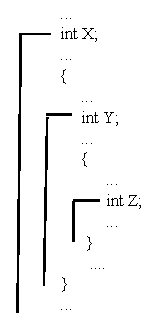
\includegraphics[width=9cm,height=6cm]{images/scope1.eps}}
\setlength{\unitlength}{1cm}
\begin{picture}(8,5)

\linethickness{0.3mm}
\put(1,4.5){\codefont{The Pet Class}}
\put(1.5,4){\codefont{hunger = }}
\put(1.5,3.5){\codefont{happy = }}
\put(1.5,3){\codefont{name = }}
\put(1.5,2.5){\codefont{pet()}}
\put(1.5,2){\codefont{play()}}
\put(1.5,1.5){\codefont{feed()}}
\put(1.5,1){\codefont{print()}}
\put(1.5,0.5){\codefont{check\_health()}}

\put(5.5,3.5){Data members; these store data for the pet objects.}
\put(5.5,1.5){Member functions (or methods);}
\put(5.5,1.0){these functions are used to manipulate the data of pet objects.}

\ifcolor\color{\mycolor}{
\put(1.25,4.4){\line(1,0){4}}
\put(1.25,0.4){\line(1,0){4}}
\put(1.25,4.4){\line(0,-1){4}}
\put(5.25,4.4){\line(0,-1){4}}
\put(1.25,2.9){\line(1,0){4}}
\ifcolor}
\end{picture}
\caption{An illustration of the \cf{pet} class.  Classes contain data members that hold information about objects of the class type (e.g., hold information about pet objects).  Classes also have member functions that act on the data.}
\label{fig:class1}
\end{figure}

\subsection{Lines 1b-49b: Defining the \cf{Pet} Class Member Functions}

Lines 1b-49b define each of the \cf{pet} class's member functions.  Each function definition begins with a line similar to those for functions in Chapter 4, but with the addition of \codefont{pet::} before the function name (lines 2b, 8b, 28b, 33b, and 39b).  This tells the compiler that these functions are part of the \cf{pet} class.  It's legal to have two functions with the same name, one that's a member of the class and one that is not.  The \codefont{pet::} denotes the function that is a member of the class.

\mysubsubsection{Lines 1b-7b: The Constructor}

A constructor\index{constructor} is a special type of member function.  A constructor is called when a new object is created.\footnote{A class can have multiple constructors, if each constructor has a different number or types of parameters.  A constructor with parameters is called like any other function, but when the object is declared.  For example, \codefont{pet pet2(7);} creates a new pet object named \codefont{pet2} using the constructor for the \cf{pet} class that has a single integer as a parameter.  If no such constructor exists, this would produce a compiler error.} A constructor has the same name as the class (e.g., \cf{pet}).  Its return type is predetermined and is not included in the program.  Thus, on line 10 and line 2b, the \codefont{pet()} function has no return type, not even \cf{void}.

On line 19 when the object called \codefont{pet1} of type \cf{pet} is created, the constructor function \codefont{pet()} is automatically called.  The pet constructor sets the new pet object's \codefont{hunger} to 50 (line 3b) and its \codefont{happy} to 50 (line 4b), and asks the user for the new pet object's name (lines 5b-6b).  The $>>$ operator reads in a string of characters up to the first whitespace character (space, tab, newline, etc.) and then stops, which is why the pet can have only one name, not a first and last name.  Later, this limitation will be removed.

Line 1b is a comment explaining what this function does.  As a comment, it does not have any effect on how the program behaves. 

\mysubsubsection{Lines 8b-26b: The \codefont{play()} Function}

This function allows the user to ``play'' with his or her pet.  Using the same basic menu structure as in Chapter 3, the user can choose to either play fetch or roll over with the pet.  Playing fetch makes the pet happier, but also hungrier (lines 16b and 17b), whereas rolling over makes the pet a little happier and only a tiny bit hungrier (lines 20b--21b).  

Note that on these lines, a new operator \codefont{+=} is being used.  The command:\\
\codefont{
happy += 10;\\
}
is equivalent to:\\
\codefont{
happy = happy + 10;\\
}
Both take the current value of the variable \codefont{happy} and add 10 to it.  The \codefont{+=} operator is just a shortcut.  Similar operators (\codefont{-=}, \codefont{*=}, etc.) are listed in Section~\ref{appendix:operators} of Appendix A.

\mysubsubsection{Lines 27b-31b: \codefont{The feed()} Function}

This function allows the user to ``feed'' the pet, thereby decreasing its hunger (here, the \codefont{-=} operator is used).
It also has the pet print some output to the user (line 29b).

\mysubsubsection{Lines 32b-37b: The \codefont{print()} Function}

This function prints information about a pet, its name, and how happy and hungry it is.  

\mysubsubsection{Lines 38b-49b: The \codefont{check\_health()} Function}

% check, has <= been used before?
This function checks the hunger (line 40b) and happiness (line 44b) of the pet.  If the pet is too hungry (hunger is larger than or equal to 100) or too unhappy (happy is less than or equal to 0), then an appropriate message declaring the demise of the pet is printed and the value 1 is returned.  If the pet is not too hungry or too unhappy, the value 0 is returned.  Note the use of the Boolean comparison operators \codefont{$<=$} and \codefont{$>=$} which stand for ``less than or equal to'' and for ``greater than or equal to'' respectively.

The return value is necessary because, in the \codefont{main()} function, the program should behave differently depending on whether the pet is alive or dead.  Currently, if the pet is alive, the program loops back to the beginning and allows the user to continue playing with or feeding the pet (lines 36 and 22), whereas if the pet dies, the program ends.  This could be changed, for example, to having the program ask if the user wants to create a new pet if the current pet dies.

\subsection{Lines 1-3 and 17-50: The Main Program}

Most of Listing~\ref{listing:electronic pet} is taken up with the \codefont{main()} function, which utilizes the \cf{pet} class.

\mysubsubsection{Lines 1-3: \#includes}
As with the previous programs, these lines are preprocessor commands for including additional libraries.  A new library, the string library, is used in this project and is included on line 2.

\mysubsubsection{Lines 19-20: Declaring variables (and objects)}

These lines declare the variables used in the \codefont{main()} function.  Two are integers: \codefont{choice} and \codefont{health\_check}.  These are assigned the values 3 and 0, respectively.  It is a good idea to assign values to variables when they are declared; otherwise, the variables hold a random value, which could cause the program to behave unpredictably.

Line 19 declares an object called \codefont{pet1} of type \cf{pet} -- the new class created for this program.  As noted above, when a new object is created, the constructor for that class is automatically called.  The constructor sets the initial values for \codefont{hungry} and \codefont{happy} for the new pet object and asks the user for a name for the pet (lines 2b-6b).

Once a class has been defined an unlimited number of objects of that type can be created.  So, although currently the program creates only one pet object (called \codefont{pet1}), many more pet objects could be created just as many variables of type \codefont{int} can be created within a program.  Each pet that's created has its own \codefont{hunger}, \codefont{happy}, and \codefont{name}.
To create more pets add a line to \cf{main()} like:\\
\codefont{pet pet2, another\_pet, X;}\\
This will create three more pet objects (with the names \codefont{pet2}, \codefont{another\_pet}, and \codefont{X}).  For each pet object, the constructor will be called, so three more pet names will be requested.  To print or play with one of the new pets, the dot notation is used: \codefont{pet2.print();} or \codefont{X.play();}\\  

\mysubsubsection{Lines 22-36: The Main Loop}

This loop is similar to the ones in both the NIM and Calculator programs.  It allows the program to repeat until either the pet dies or the user loses interest and quits.  These two conditions for ending the program are coded in the while condition on line 36.

Remember that the loop continues so long as the condition is \emph{true}.  So, the condition on line 36 can be read as \emph{while the user didn't choose option 0 (\codefont{choice != 0}) AND (\&\&) the pet is alive (\codefont{health\_check != 1}), loop back to the beginning}.

\begin{figure}
%\centerline{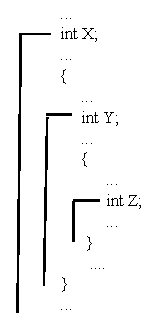
\includegraphics[width=9cm,height=6cm]{images/scope1.eps}}
\setlength{\unitlength}{1cm}
\begin{picture}(13,3)

\linethickness{0.3mm}
\put(6,1.5){\codefont{pet1.print( );}}
\put(5,2.5){object name}

\put(5.7,0.6){dot}

\put(6.1,3){function name}

\put(8,2.5){parentheses (required)}

\put(7.6,0.4){arguments (if any)}

\color{\mycolor}{
\put(5.9,2.4){\vector(1,-1){0.5}}
\put(6.2,0.9){\vector(1,1){0.5}}
\put(7.3,2.9){\vector(0,-1){1}}
\put(9.2,2.4){\vector(-2,-1){1}}
\put(8.8,0.9){\vector(-1,1){0.5}}
}

\end{picture}
\caption{The dot notation is used to call a member function of a class.}
\label{fig:memberfunctioncall}
\end{figure}

\mysubsubsection{Line 23: Printing the pet}

Line 23 calls the \codefont{print()} function of the class \cf{pet} \emph{specifically} for the object \codefont{pet1}.  Pay close attention to the general syntax of this command, which is illustrated in Figure~\ref{fig:memberfunctioncall}.  First, the name of the object is used (\cf{pet1}), then a dot (period), then the name of the function to be called (\cf{print()}).  Because this is a function, it must be followed by parentheses.  Finally, if the function expects any arguments, they are placed within the parentheses just as for other function calls.
This causes the \cf{pet} object \cf{pet1} to ``print itself,'' specifically, \cf{pet1}'s name, hunger, and happiness.  If there were a second pet object (e.g., a \cf{pet2}) it could also be asked to print itself and it would print its own values.  

\mysubsubsection{Lines 24-34: The Menu}

Lines 24-34 code a menu that allows the user to choose whether to play with or feed the pet.  First the user is prompted to enter a value (lines 24 and 25), then their choice is input (line 26), finally a switch statement is used to take the appropriate action (lines 27-34).  

If the user chooses to play with the pet (option 1) the program calls the \codefont{play()} member function using the dot notation.  If the user chooses to feed the pet (option 2) then the program calls the \codefont{feed()} member function.  
If the user enters a 0, nothing happens in the switch statement because there is no 0 case.  However, \codefont{choice} is assigned the value \codefont{0}, thus when the program reaches line 36, the program exits the main loop.

Finally, if the user enters any number other than 0, 1, or 2, nothing happens in the switch statement because there is no matching case and no default case.  When the program reaches line 36, it jumps back to the beginning of the loop because the choice is not equal to 0.  Output telling the user that he or she made an undefined choice would be helpful; adding it is one of the suggested changes.

\mysubsubsection{Line 35: Health Check}
On line 35, the program calls the \codefont{check\_health()} member function for the object \codefont{pet1}.  This function call is like the others in the program (e.g., lines 23, 29, and 32) except that the \codefont{check\_health()} member function returns a value, which is stored in the variable \codefont{health\_check} for use in the while condition on line 36.

\mysubsubsection{Lines 37-40: Graceful Exit}

Lines 37-40 use the same code as NIM to pause the program before it exits.  This is necessary in environments where the program is run in its own window, which closes as soon as the program ends.

\subsection{Public and Private}\index{public}\index{private}\index{classes!private}\index{classes!public}

The data members and member functions of a class can be either \emph{public} or \emph{private}.\footnote{There are other categories, like \emph{protected}, but they are for more advanced applications and are not covered in this text.} The public data and function members of an object can be accessed from anywhere in the code (if the object is in scope) using the dot notation.  Private members can be accessed only by other members of the class.  For example, in \cf{main()} the public \codefont{play()} member function of the \codefont{pet1} object is legally accessed on line 29.  In contrast, the private \codefont{hunger} data member is accessed (and changed) within the \codefont{play()}, \codefont{feed()}, and \codefont{print()} member functions, but it cannot be accessed directly in \codefont{main()} because \codefont{hunger} is a \emph{private} member of the \cf{pet} class.
  
To see how public and private work, add the following line to the \codefont{main()} function after line 34:\\
\codefont{pet1.hunger = pet1.hunger + 1;}\\
When this program is compiled, the compiler should produce an error message like:\\
\codefont{cannot access private member declared in class `pet'}\\
To avoid this error, the \codefont{hunger} data member can be moved from line 7 to line 11, putting it in the public declarations of the \cf{pet} class and thereby making it a public data member accessible from \codefont{main()}.  With that change, the new program should compile successfully.  

Member functions of a class can also be private.  Try moving line 14 (the declaration of the \codefont{print()} member function)  to line 8, thereby making it private.  When this program is compiled, it should also produce a compiler error like:\\
\codefont{cannot access private member declared in class `pet'}.

Change the pet program back, making \codefont{hunger} private and the \codefont{print()} member function public again.

Public and private allow the programmer of a class to control how objects of that class are used and, simplifies the work of other programmers using the class.  As an example, consider the \codefont{string} object that stores a pet's name.  In creating the \codefont{pet} class, we don't have to consider what the \codefont{string} class is doing, or how it's storing data.  So long as the functions of the class are available for review (which they are, online) and work correctly, the internal details of the class shouldn't matter.  The linking of data and functions, combined with hiding the data and accessing it only through functions, is often referred to as \emph{encapsulation}\index{encapsulation} or \emph{information hiding}\index{information hiding}.  

Encapsulation is useful because it leads to \emph{modularity}\index{modularity} -- the ability to build a complex program from code \emph{modules}\index{modules}.  Again, the \codefont{string} class is a good example.  Since its creation, the \codefont{string} class has probably been used in millions of programs by programmers who don't know what's ``inside'' the class and don't need to know, so long as its member functions work correctly.  Large software projects are often built following a similar modular process: one or more teams program the base classes, and other teams work on writing the full program using those classes as the building blocks.   
This approach to programming, using classes and objects to build a program modularly, is a form of \emph{object-oriented programming}\index{object-oriented programming (OOP)} (\emph{OOP}\index{OOP}) and is one of the dominant programming paradigms in use today.

In general, it is a good idea to make the data members of a class private.  This makes it very difficult for someone using the class to accidentally set a bad value (e.g., setting a pet's happiness to -1000 or putting a zero in the denominator of a fraction class) because the public member functions that are used to access the data can check the values before they are set and make sure they make sense.   The member functions of a class are generally public to give access to the class data members, but classes often include private functions that can be called only by other members of the class.  The project in Chapter 7 includes a class with several private member functions.


\vspace{+0.25cm}
{\color{\mycolor}\noindent\hrulefill}
\section{Exercises: Modifying the Program}

The current Electronic Pet program is not particularly complex.  There are a few menu options and a pet's hunger and happiness levels vary, but there's not much to hold a user's interest for more than a few minutes.  However, the code contains the basic framework for a much more interesting program. 

\mysubsubsection{Exercise 1: The Main Menu}

There are a number of places where the output should be improved.  
In the switch statement in the member function \codefont{play()}, there is a default case (line 24b) that tells the user when he or she has made an invalid choice.  Add a similar default case to the switch statement in the main program (e.g., after line 33) to warn the user if they make an invalid selection.  Also add a \codefont{case 0} for when the user chooses to exit the program.  In general, it's a good idea to have a case for every expected option, even if the case doesn't do anything in the current program.  Additionally, when the default case is added, the \codefont{0} case will incorrectly jump to it, unless there is a separate case for when the user enters a \codefont{0}.

\mysubsubsection{Exercise 2: More Interactive Pets}

When the user chooses to feed the pet he or she gets a message in response: ``MMM, Yummy!'' (line 24b), which makes the program more interactive.  But no such message occurs when the user plays with the pet.  Add similar messages to the \codefont{play()} member function.  Placing them within the switch statement (e.g., after lines 17b and 21b), allows different messages depending on the user's choice.  

\mysubsubsection{Exercise 3: More Interesting Output}

Modify the \codefont{print()} member function to give more interesting output.  Instead of simply printing the values of \cf{happy} and \cf{hungry}, use an \codefont{if} statement to print messages that are more appropriate to the pet's level of happiness and hunger.  For example, adding:\\
\codefont{
if(hungry > 80 \&\& hungry < 90)\{\\
\hspace*{0.5cm} cout $<<$ "I'm starving!  Feed me!\textbackslash n";\\
\}\\
}
to the \codefont{print()} member function will make the pet ``respond'' based on its \cf{hunger} level.  Use a series of similar conditionals for different values of \codefont{hungry} and \codefont{happy} to create more interesting output.

\mysubsubsection{Exercise 4: Randomized Output}

The \codefont{feed()} member function always prints the same message every time the pet is fed.  Use a random number and a switch statement to make the pet print a variety of messages when it is fed.  

\mysubsubsection{Exercise 5: More Play Options}

When a user chooses to play with the pet he or she only has two options: to play fetch or roll over.  Expand the number of cases in the switch statement (lines 14b-25b) to give the user more ways to play with the pet.  (Don't forget to include any new options in the output on line 12b.)

\mysubsubsection{Exercise 6: More Feed Options}

Currently, there's only one action associated with feeding the pet; hunger decreases by 5.  Modify the \codefont{feed()} member function to give the user different options for feeding the pet (like the \codefont{play()} member function, which gives the user a several ways to play with a pet).  For example, options could include feeding the pet generic food that decreases hunger, but also decreases happiness; or regular food that only decreases hunger; or fancy food that decreases hunger and increases happiness.  To make this change, add a switch statement, like the one on the \codefont{play()} member function, to the \codefont{feed()} member function.

\mysubsubsection{Exercise 7: Longer Pet Names}

Currently, a pet's name can only consist of a single word (e.g., ``Bob'' or ``Fluffy'').  This is because the input operator $>>$ reads characters only up to the next whitespace.  If the user enters a name like ``Bob P. Fluffles,'' only the ``Bob'' is read -- the rest of the name remains in the input buffer and causes problems later in the program.  The \codefont{string} class has a number of functions that can solve this problem.  The simplest is \codefont{getline(istream, string)} which reads a string of characters up to a newline character (`\textbackslash n') from the \codefont{istream} argument and stores them in the \codefont{string} argument.  Use this function to allow pets to have longer, multipart, names.  (An alternative approach would be to declare several new data members as part of the pet class: \codefont{first\_name}, \codefont{last\_name}, etc.  But it's trickier to get this to work smoothly if the pet's name has a variable numbers of parts: first, last, middle, title, etc.)

\mysubsubsection{Exercise 8: Give Pets a Species}

Add a new data member that stores the type or species of the pet.   The new data member should be of type \codefont{string} like the \codefont{name} data member.  The new data member should be added around lines 7-9, where the other data members are declared.  In addition, the user will need to enter the type of the pet as part of the constructor member function (lines 2b-7b) and the \codefont{print()} member function should print each pet's type (around line 34b).

\mysubsubsection{Exercise 9: Other Pet Qualities}

Expand the \cf{pet} class with at least one additional data member that defines another aspect of the pet's well-being.  For example,  a health data member or a tiredness data member.  Add the data member to the class definition (around line 9), set the initial value as part of the constructor (around line 4b), and make sure the new data member is printed in the \codefont{print()} member function (around line 34b).  Modify the existing member functions to affect the new data member; for example, playing fetch makes a pet healthier \emph{and} more tired.

Add a new member function to manipulate the new data member.  For example, a \codefont{rest()} member function to make the pet less tired, or a \codefont{vet\_visit()} member function to make the pet healthier (and probably less happy).  Include the new member function as part of the class definition (around line 15) and the code for the new function (probably after line 49b, although as a new function, it could be placed anywhere after \codefont{main()}).  A simple way to create new member functions is to copy an existing member function and then modify it, starting by changing the function's name, and then its code.  Add a new option to the main menu to allow the player to choose the new function.

\mysubsubsection{Exercise 10: More Pets}

Add another pet for the user to interact with. 
It is simple to create more than one pet object by adding more pet declarations; for example, \codefont{pet second\_pet;} which creates another pet object named \codefont{second\_pet}.   
Interacting with a second pet object requires statements like: \codefont{second\_pet.play();} and
\cf{second\_pet.feed();}.  
One approach is to copy the switch statement (lines 23 to line 36), then change the pet variable in the second copy, so the user can interact with both of them.  Another approach is to have the program ask the user which pet they want to play with and then use a conditional on the user's choice to select which pet calls the member function.  Something like:\\
\cf{
if(pet\_choice == 1)\{\\
\hspace*{2cm}pet1.play();\\
\}\\
else if(pet\_choice == 2)\{\\
\hspace*{2cm} pet2.play();\\
\}\\
}
Additional changes are required to handle the case where one pet dies and not the other.  (One approach would be an if statement that only allows the user to interact with a pet object only if it passes a health check.)  The next two chapters will introduce data structures that will make it easier to have multiple pets.

\section{Files}\index{files}
\index{close()@{\cf{close()}}}\index{files!close()@{\cf{close()}}}
\index{write}\index{files!write}
\index{read}\index{files!read}

A clear weakness of the Electronic Pet program is that the user can play with a pet only once.  As soon as the program ends, the pet is lost.  This problem can be fixed by using a \emph{file} to store the information about a pet when the program is not running.  In C++, files are accessed using \codefont{fstream} objects (short for \emph{f}ile \emph{stream}).  Typically, an \codefont{ifstream} object (short for \emph{i}nput \emph{f}ile \emph{stream}) is used to read from a file and  an \codefont{ofstream} object  (short for \emph{o}utput \emph{f}ile \emph{stream}) is used for writing to a file. 
File stream objects must open a file before they can send or receive data.  After a file is opened, the program can write to it or read from it using the same operations as are used with \codefont{cin} and \codefont{cout} (e.g., $<<$ and $>>$).  After a program is done using a file, it should close the file.  For example, the code\\
\codefont{
ofstream outfile;\hspace{4cm}\emph{\textbackslash\textbackslash create an ofstream object}\\
outfile.open("filename");\hspace{2.3cm}\emph{\textbackslash\textbackslash Open the file ``filename''}\\
outfile $<<$ "Some text" $<<$ endl; \hspace{0.6cm}\emph{\textbackslash\textbackslash Write some text}\\
outfile.close(); \hspace{4cm}\emph{\textbackslash\textbackslash Close the file}\\
}
opens\index{open()@{\cf{open()}}}\index{files!open()@{\cf{open()}}} a file called ``filename'' for output, writes the string ``Some text'' followed by a new line to the file, and then closes the file.  A similar process is used to open a file to read from it.  For example, the code:\\  
\codefont{
ifstream infile;\hspace{4cm}\emph{\textbackslash\textbackslash create an ifstream object}\\
int x; \\
infile.open("filename");\hspace{2.1cm}\emph{\textbackslash\textbackslash Open the file ``filename''}\\
infile $>>$ x; \hspace{4.3cm}\emph{\textbackslash\textbackslash Read one integer from the file}\\
infile.close();\hspace{4.1cm}\emph{\textbackslash\textbackslash Close the file}\\
}
opens a file called ``filename'' for input, reads a single integer from the file, and then closes the file.  
Modifiers to the \codefont{open()} function allow a file to be opened for appending or to write over the existing file.  If the program attempts to open a file for output and the file doesn't already exist, the program will attempt to create the file.

\mysubsubsection{Exercise 11: Saving a Pet}

Modify the Electronic Pet program to write a pet's data to a file when the program ends and read a pet's data from a file when the program begins.  
The following changes make this possible.  First, when a new pet object is created, the program needs to ask the user whether to create a brand new pet or to load the data for an existing pet from a file.  If the user wants to load a pet, then the program should ask for the pet's name, create an \codefont{ifstream} object,  use the \codefont{ifstream} object to open the file and read the pet information from the file.  For example,\\
\cf{
cin >> name;\hspace{4cm}\emph{\textbackslash\textbackslash get the pet's name, used as the file name}\\
instream infile;\hspace{3.2cm}\emph{\textbackslash\textbackslash create the infile object}\\
infile.open(name.c\_str());\hspace{1.25cm}\emph{\textbackslash\textbackslash open the file\footnote{The \cf{open()} function expects a C-style string (see Interlude 4) not a string object; the \cf{c\_str()} function returns the correct type to the \cf{open()} function.}}\\
infile >> hunger;\hspace{3.1cm}\emph{\textbackslash\textbackslash read the pet's data}\\
... \\
infile.close();\hspace{3.6cm}\emph{\textbackslash\textbackslash close the file}\\
}
Similarly, when the program ends, it should save the data, by creating an \codefont{ofstream} object, opening a file, and writing the pet's data to the file.  Make sure that the data is written to the file in the same order that it is read from the file, otherwise the values of \cf{hunger} and \cf{happy} (for example) may end up switched every time the program is run.

This example uses the pet's name as the file name.  Alternatively the program could ask the user for a file name.

There is one tricky part to opening files.  The file \codefont{open()} function expects the name of the file as a C-style string (covered in Interlude 5), not a \codefont{string} object. If the file name is stored as a \codefont{string}, then a member function of the string class named \codefont{c\_str()} must be used to get the file's name in the right format.  For example:\\
\codefont{infile.open(filename.c\_str());\\}
where \codefont{infile} is an object of type \codefont{ifstream} and \codefont{filename} is an object of type \codefont{string}.

The stream classes include a number of member functions that are useful for accessing data in files, checking whether a file opened correctly, etc.  A few of the most common functions are listed in Section~\ref{appendix:iostream} of Appendix A.

\section{Problems}
It's important to remember that classes are a general way to define any type of object, not just pets.  The programmer can include many different data members or member functions in a class.  This makes classes almost infinitely flexible.  
\begin{enumerate}

\item {\bf Pet Game}\\
 The Electronic Pet program can be turned into a ``real'' game by making it more challenging to balance the pet's different needs.  Add new pet qualities, like health and tiredness, as discussed previously (Exercise 9).  Modify the behaviors so that each user choice increases some values, but lowers others (e.g., playing increases happiness, but also increases hunger and tiredness) so that keeping a pet healthy and happy is a balancing act.

\item {\bf Random Outcomes}\\ 
Currently, the outcomes of user choices are fixed; feed the pet and \codefont{hunger} goes down by a fixed amount (although the user, not having read the code, might not know by how much).  Instead (partially) randomize the outcomes.  For example, feeding a pet lowers \codefont{hunger} by a random amount, and may, in rare cases, make the pet less healthy (e.g., the user got some bad pet food).  Put in appropriate output so the user knows what is happening.  These changes should make the pet game more challenging to play.

\item {\bf Pet Game with Money}\\
To make the pet game even more interesting, add money as a pet quality.  Add options like working or entering competitions, that allow the pet to earn money.  Make actions like buying pet food or toys, or going to the vet, cost money.  

\item {\bf Random Events }\\ Add random events to the program so that every time the user finishes an action, there's a chance that a random event occurs that affects the status of the pet.  This requires a new member function that is called once per loop (like the \codefont{print()} member function).  The function should use at least two random numbers, one to determine if an event occurs and one to determine what event occurs. Example events might include the pet getting injured (lowers health and happiness) or rescuing little Timmy (increases happiness).\footnote{One of the first widely successful video games, The Oregon Trail\texttrademark, originally released in 1974, was based on the same framework of selecting actions to balance resources combined with randomized impacts and events.  Versions of The Oregon Trail continue to be released, and resource balancing in one form or another is an important aspect of many computer games.}

\item {\bf Names in NIM}\\
Change the NIM project so that players can enter their name.  Have the game refer to the player by name instead of saying ``Player 1.''

\item {\bf Files in NIM}\\
Change the NIM project so that it uses a file to keep track of how many times a player has won and lost.  Each time the game starts it should ask the player if they are a new player.  If they are a new player the game should ask them for a new username to store for their record of wins and losses.  If they are a returning player they should enter their previous username and use that to open the correct file.  (Assume that every player will have a unique user name.)  

\item {\bf Spaceship}\\ 
Create a new resource balancing game (for the pet, the resources are happiness, hunger, etc.)  based on flying an interstellar spacecraft to a nearby solar system.  Make the user balance resources like fuel use, oxygen supply, crew happiness, distance traveled, etc.

\item {\bf Planet Game}\\ Create a game that requires balancing the resources of a whole planet (or solar system, universe, multiverse, etc.).

\item {\bf Bank Account}\\ 
A similar structure can be used for nongame applications.  Instead of a \cf{pet} class, create a bank account class with \codefont{checking} and \codefont{savings} as data members.  Instead of play and feed, the user can choose to deposit, withdraw, or transfer to money to savings.  For each action the user will need to input how much money was deposited, withdraw, etc.  The \cf{print()} function should print the current balance in checking and in savings.


%\item Tracking Goals - Very generally, a program with a structure similar to the pet program can be used to track any goal.  For example, the program could be used to track progress towards an A in a course.  Every time the user gets an assignment or a test back they enter it like it was a behavior (instead of feeding their pet, they would finish an assignment) increasing their score/grade.  The program should include positive feedback when the user enters a good score.
\end{enumerate}





\addtocounter{interlude}{1}
\setcounter{section}{0}
\setcounter{figure}{0}
%********** Interlude **********
\interlude{Software Design and Engineering}

When starting a new program, particularly a large, complex piece of software, it is important to begin with a design.  No one would start constructing an automobile, a building, or any other complex device or structure without a clear set of designs or blueprints.  Writing software is no different.  Starting the process of writing a complex program by sitting down and typing ``int main'' is almost a guarantee of failure.   In terms of the number of active, interacting parts (variables, functions, etc.), a software program is just as complex as the largest machines or buildings.  Thus, in building a complex program, or even a fairly simple one, it is critical to have a reasonable design for the program before coding begins.

Many techniques and approaches for designing software have been developed.  \emph{Software engineering}\index{software engineering} is the application of a structured approach to the design, coding, testing, and maintenance of software.  Software engineering is an important field within computer science and most computer science programs include courses on software design and engineering.

Two common, general approaches to software design are \emph{top-down}\index{top-down} design and \emph{bottom-up}\index{bottom-up} design.  Both of these can be applied using very rigorous, well-defined methodologies, but they can also be applied informally, as general guidelines for the design of a program.  The informal approach is useful for relatively small programs as in this text.

Top-down design begins by focusing on the high-level structure of the program.  The designer outlines, often using diagrams or flow charts, how the overall program will ``flow.''  Programming starts with this high-level picture.  For example, in the Electronic Pet project a top-down approach would start by designing the main program loop and then designing the \cf{pet} class.  Similarly coding starts with the main program loop, using \emph{stub code}\index{stubs} in the place of complex blocks of code and functions.  Stub code is simply code that acts as a temporary placeholder.  For example, in the Electronic Pet project, a programmer might initially write the \codefont{play()} member function to just print the word ``play'' and the \cf{feed()} function to just print the word ``feed.''  This is easy to write and allows the programmer to make sure that the overall program works, before worrying about filling in the details.  

Only after the main program loop was working would the programmer go back and start filling in the details of the \cf{pet} class and its functions.

Bottom-up design begins by putting together the ``building blocks'' of a program.  For example, in the Electronic Pet project, a bottom-up approach would start with designing and writing the \codefont{pet} class.  Once the \codefont{pet} class was complete, then the rest of the program would be written to use it.  A bottom-up approach is often used when a very specific class is required.  For example, if a programmer wanted to create a program that dealt with fractions or virtual pets, he or she might begin by creating the fraction or pet class and then write the rest of the program to use the class.  

Of course, it is not necessary to strictly adhere to either a top-down or bottom-up approach -- for small projects, many programmers prefer a hybrid.  They might begin by sketching (often literally) the broad program in a top-down design, but then start by coding the bottom-level classes. 
Or they might code a stub version of the classes first, then write the top-level code using the stub class, and finally fill in the class details.  

Another important aspect of software engineering is careful specification of what the parts of the program, the functions, classes, etc., should do.  Specifications typically include input types, output types, behaviors, and special cases.  If a program is well designed, with each piece correctly specified in advance, then it's comparatively simple to write each piece of code to match the specifications and end up with a complete program.  In addition to specifications, a good design includes test cases -- specific sets of tests that are paired with the specifications.  When a piece of code is written it is tested using the predefined test set to confirm that it functions as specified. 

In designing a program, it is often very helpful to sketch it on paper.  For example, a programmer drawing boxes to represent the major components of the program (classes, functions, etc.) and adding lines and arrows showing how these components interact.  Even a very simple sketch can help clarify how a program is supposed to work and serves as a reference when writing each of the program's components.

%Another common tool for program design is a flowchart\index{flowchart}.  A flowchart is a specific way to define how a program behaves.  Figure~\ref{fig:flowchart} illustrates a flowchart for the NIM program.

As programs become more complex and involve larger teams, having a good design becomes increasingly critical.  A good design helps to make sure that all of the programmers are working towards a common goal.  Many software companies have their own design (and testing) methodologies that their programmers are required to use.  Although strict software design methodologies can seem cumbersome and a hindrance to actual programming, they are important for keeping large projects on track.  However, at this stage in learning to program, the most important thing is to try out some of the basic design methods to see which ones fit your programming style.






%\addtocounter{chapter}{1}
\setcounter{section}{0}
\setcounter{figure}{0}

%********** Chapter 6 **********
\chapter{Generic Board Game}\index{Generic Board Game}\index{projects!Generic Board Game}\label{ch:boardgame}

\section{Introduction}

This chapter introduces the fourth project: a generic board game.  In this game, two players roll a simulated die to move along a board trying to get to the goal.  Along the way, they land on squares that may either move them backwards or forwards.  The game has the same general format as  Candyland{\texttrademark}, Chutes (or Snakes) and Ladders{\texttrademark}, Life{\texttrademark}, and similar board games.  Like the earlier projects, the initial version of the program is generic, just the general framework for a board game, but it is designed to be easy to modify to meet the programmer's needs and interests.

This project reviews the topics from the earlier chapters, particularly classes, scope, and files, and introduces several new topics:
\begin{tight_itemize}
\item Pass-by-reference\index{pass-by-reference}\index{arguments!pass-by-reference}
  \item Arrays\index{arrays}
  \item Characters (the \cf{char} type)\index{characters}\index{char@{\cf{char}}}\index{type!char@{\cf{char}}}
  \item Global variables\index{globals}
   \item Constants\index{constants}
\end{tight_itemize}

 Pass-by-reference is an alternative method of passing arguments to functions, it allows changes made to the function's parameters to persist in the calling function.  Arrays are data structures that store multiple data of the same type; for example, a list of integers or doubles or objects of the same type.  They are one of the most widely used, and useful, of the basic data structures.  Characters, abbreviated \codefont{char} in code, are a new type that stores a single character: `a', `b', `=', `5', etc.  Global variables are variables whose scope extends throughout the entire program.   Constants are named boxes that store values that cannot change.

\section{The Program}

Listings~\ref{listing:GenericGameA},~\ref{listing:GenericGameB}, and~\ref{listing:GenericGameC} present the code for the board game.  In addition, this program requires data, which is read from a file.  Listing~\ref{listing:game.txt} presents the initial data file.  


To compile and run the program, enter the code from Listings~\ref{listing:GenericGameA},~\ref{listing:GenericGameB}, and~\ref{listing:GenericGameC} (but not Listing~\ref{listing:game.txt}) in that order into a single program\ (do \emph{not} enter the line numbers).  Try to figure out what the statements do.  Many of them should be very familiar by now, but others will be new.

\begin{minipage}{\textwidth}
\begin{lstlisting}[language=C++,numbers = left,xleftmargin=4.0ex, basicstyle=\small, emph={move,message,symbol,board_length},emphstyle = \color{\mycolor}, 
showstringspaces=false,
caption = {Initial code for the Generic Board Game program, including the include statements, declaration of the \cf{square class}, prototypes for the other functions defined as part of the program, and a global constant called \codefont{board\_length}.},
label={listing:GenericGameA}]
 #include<iostream>
 #include<string>
 #include<fstream>
 #include<ctime>
 #include<cstdlib>
 using namespace std;
                            // Declaration of the square class
class square{
  private:
     int move;
    string message;
    char symbol;
  public:
    square();
    void print();
    int action();
    void set(int,char,string);
};
                            // Function Prototypes
void print_board(square[], int, int);
void read_board(square[]);
void check_position(int &);
                           // Global variables
const int board_length = 20;
\end{lstlisting}
\end{minipage}

Next, create a plain text file called ``game.txt'' containing the text from Listing~\ref{listing:game.txt}.  This file should be in the same directory or folder as the program file.

Once the entire program has been entered and the data file ``game.txt'' has been created, compile the program.  As always there may be some copying errors that need to be fixed.  Once the program compiles, run it.  Try to figure out what the data file is used for.

As with the other projects in the text this program has some shortcomings.  Most notably it is, as advertised, a generic game.  However, the program is written to make it very easy to customize.  Instead of game with generic messages like ``Go back 2 squares'' it can be turned into a specific game. For example, a sailing game with messages like ``Strong currents push your ship backwards'' or ``Good winds advance 2 squares.''  As explained later in the chapter, giving the game a specific theme only requires changing the file ``game.txt.'' 

\subsection{Pass-by-reference}\index{pass-by-reference}\index{arguments!pass-by-reference}\index{functions!pass-by-reference}

Functions, arguments, and parameters were introduced in Chapter 3.  ``Standard'' function parameters are pass-by-value: the value of the arguments are copied into the function.  An alternative approach is \emph{pass-by-reference}.  In pass-by-reference, a \emph{reference} to the ``box'' holding the argument is passed to the function rather than the argument's \emph{value}.\footnote{The reference is actually the \emph{address} in memory where the argument is stored.  Because the function receives the address in memory of the variable it can change the value directly.  Addresses and memory are discussed in more detail in Chapter 7.} This means that the function has direct access to the ``box'' holding the argument value in the calling function.   Figure~\ref{fig:passbyrefarguments} illustrates this idea.  Any changes that the function makes to an argument persists after the function exits, even if the new value is not returned by the function.  

\begin{minipage}{\textwidth}
\renewcommand*\thelstnumber{\the\value{lstnumber}b}
\begin{lstlisting}[language=C++,numbers = left,xleftmargin=4.0ex, basicstyle=\small, emph={current_player,player1_position,player2_position,the_board},emphstyle = \color{\mycolor},
showstringspaces=false,breaklines=true,
  breakatwhitespace=true,
caption = {The \codefont{main()} function for the Generic Board Game.},
label={listing:GenericGameB}]
int main(){
  int current_player = 1, roll;
  int player1_position = 0, player2_position = 0;
  square the_board[board_length];  // declare an array of squares
  srand(time(NULL));
  read_board(the_board);
  print_board(the_board,player1_position,1);
  print_board(the_board,player2_position,2);
  do{
      cout<<"\n\n\nPlayer "<<current_player<<" type enter to roll.\n";
      cin.ignore();
      roll = 1 + (rand() % 5);
      cout << "Player "<<current_player<<" rolled a "<<roll<<".\n";
      if(current_player == 1){
         player1_position += roll;
         check_position(player1_position);
         player1_position += the_board[player1_position].action();
         check_position(player1_position);
      }
     else{
        player2_position += roll;
        check_position(player2_position);
        player2_position += the_board[player2_position].action();
        check_position(player2_position);
     }
     print_board(the_board,player1_position,1);
     print_board(the_board,player2_position,2);
     current_player = (current_player % 2) + 1;
  }while((player1_position<board_length-1) && (player2_position<board_length-1));
  current_player = (current_player % 2) + 1;
  cout << "\nPlayer " << current_player << " Wins!!!\n";
  cin.ignore();
  return 0;
}
\end{lstlisting}
\end{minipage}

To create a pass-by-reference parameter, an \& symbol is put after the parameter type in both the function prototype and function definition.  In the Generic Board Game, the \codefont{check\_position()} function uses pass-by-reference -- note the use of the \& symbol on lines 22 and 26c to indicate pass-by-reference.  The \codefont{check\_position()} function checks the position of the user on the board, and if it isn't on the board, changes the position to be back on the board.  The function doesn't return the new position, but because the position was passed to the function as a pass-by-reference argument, the changes made within the function apply to the variable that was passed to the function.  Thus, the variable \codefont{player1\_position} on line 16b may be different after the \codefont{check\_position()} runs.

\begin{minipage}{\textwidth}
\renewcommand*\thelstnumber{\the\value{lstnumber}c}
\begin{lstlisting}[language=C++,numbers = left,xleftmargin=4.0ex,basicstyle=\small, emph={current_player,player1_position,player2_position,the_board},emphstyle = \color{\mycolor},
showstringspaces=false,
caption = {The function definitions for the Generic Board Game program.  Some are general functions, while others are member functions of the \cf{square} class.},
label={listing:GenericGameC}]
void read_board(square b[]){
     ifstream infile;
     infile.open("game.txt");
     int square_number, square_move;
     string square_message;
     char square_symbol;
     while(!infile.eof()){
         infile >> square_number >> square_move >> square_symbol;
         getline(infile,square_message);
         if(square_number < board_length)
               b[square_number].set(square_move,square_symbol,square_message);
     }
}
void print_board(square b[], int player_position, int player_number){
     for(int i = 0; i < board_length; i++){
         if(i != player_position)
             b[i].print();
        else
             cout << player_number;
    }
    cout << "Goal\n";
    for(int i = 0; i < board_length; i++)
         cout << "-";
    cout << "\n";
}
void check_position(int &p){
    if(p < 0)
         p = 0;
    if(p >= board_length)
         p = board_length-1;
}
                           // Functions of the class square
square::square(){
     symbol = ' ';
     move = 0;
     message = "";
}
int square::action(){
     cout << message << endl;
     return move;
}
void square::print(){
     cout << symbol;
}
void square::set(int m, char s, string a_message){
     move = m;
     symbol = s;
     message = a_message;
}
\end{lstlisting}
\end{minipage}

\begin{minipage}{\textwidth}
\renewcommand*\thelstnumber{\the\value{lstnumber}d}
\begin{lstlisting}[language=C++,numbers = left, xleftmargin=4.0ex, basicstyle=\small,emph={},emphstyle = \color{\mycolor},
showstringspaces=false,
caption = {The data for the file ``game.txt.''},
label={listing:game.txt}]
   7 -2 ? Go back 2 squares.
   4 +1 * Go ahead 1 square.
\end{lstlisting}
\end{minipage}

Pass-by-reference has advantages and disadvantages.  Because the changes to the argument are persistent, it is not necessary to have the function return a value and it is possible to change the value of several arguments in one function.  However, functions that use pass-by-reference should only change an argument's value in ways that are meant to be persistent and that are expected.  Otherwise, there's a risk of overwriting important data or confusing a programmer who's using the function and didn't expect their argument's values to change.
Pass-by-reference is most useful when a function is expected to change or return multiple values.  If only one value needs to be changed, regular pass-by-value arguments and a single return value can, and should, be used.


\begin{figure}
%\centerline{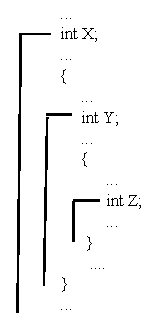
\includegraphics[width=9cm,height=6cm]{images/scope1.eps}}
\setlength{\unitlength}{1cm}
\begin{picture}(12,5.5)
\codefont{
\put(0.2,4.5){int main()\{}
\put(0.5,4.0){int x = 7;}
\put(0.5,3.5){int y;}
\put(0.5,3.0){y = foo(x);}
\put(0.5,2.5){...}
%\put(0.5,2.0){\\ x may have changed}
\put(0.2,1.0){\}}
}
%\put(4.1,3.6){\vector(1,0){5.5}}
\put(4.2,4.8){The box for \codefont{x} is \emph{shared} with the }
\put(4.0,4.3){function \codefont{foo()} under the new name \codefont{z}.}

\put(6.6,3.4){7}
\put(6.4,3.9){\codefont{x}}

\put(3.6,2.4){12}
\put(3.4,2.9){\codefont{y}}

\put(0,0){\large\textbf{main() and its variables}}
% ----------------  func
\codefont{
\put(11.5,4.5){int foo(int \&z)\{}
\put(11.8,4.0){int a;}
\put(11.8,3.5){a = z + 5;}
\put(11.8,3.0){...}
\put(11.8,1.5){return a;}
\put(11.5,1.0){\}}
}

\put(4.4,2.3){The \emph{value} of \codefont{a} is copied into \codefont{y}}
\put(4.4,1.8){when the function returns.}

\put(6.9,3.9){\codefont{z}}

\put(10.1,2.4){12}
\put(9.9,2.9){\codefont{a}}
\put(10.5,0){\large{\textbf{foo() and its variables}}}

\ifcolor\color{\mycolor}{
\put(9.8,2.7){\vector(-1,0){5.5}}
\put(13.35,5.38){\vector(1,-1){0.5}}
\put(3.5,2.3){\line(1,0){0.5}}
\put(3.5,2.8){\line(1,0){0.5}}
\put(3.5,2.3){\line(0,1){0.5}}
\put(4.0,2.3){\line(0,1){0.5}}
\put(10,2.3){\line(1,0){0.5}}
\put(10,2.8){\line(1,0){0.5}}
\put(10,2.3){\line(0,1){0.5}}
\put(10.5,2.3){\line(0,1){0.5}}

\put(6.5,3.3){\line(1,0){0.5}}
\put(6.5,3.8){\line(1,0){0.5}}
\put(6.5,3.3){\line(0,1){0.5}}
\put(7.0,3.3){\line(0,1){0.5}}
\ifcolor}

\end{picture}
\caption{When a function parameter is \emph{pass-by-value}, denoted by the \& symbol in the function's parameter declaration, the variable's ``box'' is ``shared'' between the functions.  Any changes to the parameter's value in the function ``persist'' in the calling function.  Returned values are still copied as normal.  Contrast this to the illustration of pass-by-value in Figure~\ref{fig:arguments} in Chapter 4.}
\label{fig:passbyrefarguments}
\end{figure}

\subsection{Arrays}\index{arrays}

In programming, it's often useful to store many values of the same type.  For example, a list of grades, telephone numbers, baseball scores, etc.  The simplest method to store a list of data is to use an array -- a set of data items, all of the same type, stored sequentially in memory.  
Figure~\ref{fig:array1} illustrates this idea.

Arrays are declared and accessed using square brackets: [ and ].  The general form of an array \emph{declaration} is:\\
\codefont{type name[\emph{N}];}\\
where \codefont{type} is the type of data to be stored, \codefont{int}, \codefont{string}, class, etc.; \codefont{name} is the name of the array; and \codefont{\emph{N}} is the size of the array (i.e., the number of elements the array can hold).  For example, the command:\\
\cf{double values[10];}\\
creates an array that can hold 10 values of type \cf{double}.


The elements of an array are numbered starting from 0.  So, in an array of \codefont{\emph{N}} elements, the elements are numbered from $0$ to \codefont{\emph{N}-1}.  

The general form of a statement to access an array element is:\\
\codefont{\emph{name}[\emph{index}]}\\
where \codefont{\emph{name}} is the name of the array and \codefont{\emph{index}} is the number of the particular item in the array that needs to be accessed.  For example, the command:\\
\codefont{values[3] = 7.7;}\\
sets the \emph{fourth} item in the array called \codefont{numbers} to the value 7.7 and the command:\\
\cf{cout << values[2];}\\
prints the \emph{third} element of the array (because arrays start with element 0).   The index used to access an element of an array can be an integer, an expression, or an integer variable.

Array elements can be accessed \emph{only} one at a time.  For example, copying one array into another requires a loop that copies each element individually; printing an array requires printing each element individually.  

\subsection{Array Bounds}\index{arrays!bounds}

\begin{wrapfigure}{R}{0.5\textwidth} \framebox[\linewidth][l]{\parbox{0.95\linewidth}{\codefont{Out of Bounds Errors and Security} \\
Out of bounds errors are often exploited by hackers to break into programs.  Consider a program that asks the user for a password and stores it in an array.  If the program is not well written, a clever hacker can enter a long password that exceeds the size of the array.  Doing this causes some of the password characters to be written into other parts of memory.  If the over-sized password is carefully designed, some of the characters in the password may be written into, and thereby change, the variable that determines whether the password is correct.  This tricks the program into thinking that a valid password was entered and allows the hacker entrance into the system.  Modern, well-designed systems avoid this problem by only reading as many characters as they can safely store, regardless of how many characters the user actually enters.
}}
\vspace{-0.5cm}
\end{wrapfigure}

When an array is declared in C++, the program sets aside enough contiguous memory to hold the whole array and uses the array name as a pointer to the beginning of the block of memory.  For example, if a program declares an array of 100 integers called \codefont{data}, then the program sets aside enough memory to hold 100 integers and the variable \codefont{data} points to the first element in the array.\footnote{The variable literally stores a number corresponding to the \emph{memory address} where the first element of the array is stored.  Pointers and memory addresses are covered in more detail in the next chapter.}

To access an element of an array, a program starts at the first element of the array and then jumps to the memory location indicated by the index.  For example, the command:\\
\codefont{data[7]}\\
tells the program to start at the location in memory that \codefont{data} points to and then jump forward in memory by seven integers' worth of memory (assuming \codefont{data} is an array of integers) and grabs whatever data is found in that memory location.\footnote{This is why arrays start counting from 0, the array name points to the first element of the array, so a size 0 jump reaches the first element.}

The critical idea is that a C++ program does \emph{not} check whether the place it jumps to is actually within the array.  From the compiler's point of view, it is perfectly acceptable to create an array of 10 elements and then try to access the $11^{th}$ element, or the $1,000^{th}$ element, or even the $-10^{th}$ element.  Trying to access an array element that is not within the range of the array elements is commonly known as an \emph{out of bounds}\index{out-of-bounds}\index{errors!out-of-bounds} error.

%\begin{wrapfigure}{R}{0.5\textwidth} \framebox[\linewidth][l]{\parbox{0.95\linewidth}{\codefont{Creating Libraries} \\
%All of the projects in this text are entered as a single, long program.  More commonly programs are broken up into the main program file and separate libraries.  In the case of the Generic Game program it would be common to put the square class in a separate library.  Generally, this requires putting the code into a separate file and `including' it as an additional library.  However, depending on the programming environment the actual steps may vary, Visual Studio has a specific `add a class' menu option whereas using a command line compiler requires creating the files.  To avoid having to detail multiple approaches all programs are treated as a single file in this text, but you are encouraged to figure out how to break them into separate libraries in your particular programming environment.
%}}
%\vspace{-0.5cm}
%\end{wrapfigure}

Out of bounds errors generally have one of two effects on a program.  If the program tries to access a piece of memory that is too far out of an array, it may end up trying to access a region of memory that the program does not have access to, in which case the operating system forces the program to stop running.\footnote{When a program starts running, the operating system assigns the program its own region of memory to work in; the program is not allowed to go outside this region to keep it from interfering with any other programs.}  Typically, the program crashes and the operating system prints a ``segmentation fault'' message, meaning that the program has stepped outside its allowed segment of memory.  


\begin{figure}
%\centerline{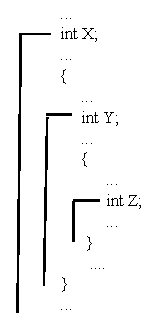
\includegraphics[width=9cm,height=6cm]{images/scope1.eps}}
\setlength{\unitlength}{1cm}
\begin{picture}(12,3.5)
\linethickness{0.3mm}

\put(6,2.8){\codefont{numbers[0]} \hspace{0.4cm}5}
\put(6,2.3){\codefont{numbers[1]} \hspace{0.4cm}6}
\put(6,1.8){\codefont{numbers[2]} \hspace{0.4cm}99}

\put(6,1.3){\codefont{numbers[3]} \hspace{0.4cm}2}

\put(7,0.8){... \hspace{0.8cm} ...}
\put(6,0.25){\codefont{numbers[9]} \hspace{0.4cm}8}

\put(11.3,2.8){\cf{numbers}}

\color{\mycolor}{
\put(8,0.7){\line(1,0){1}}
\put(8,1.2){\line(1,0){1}}
\put(8,1.7){\line(1,0){1}}
\put(8,2.2){\line(1,0){1}}
\put(8,2.7){\line(1,0){1}}
\put(8,0.2){\line(1,0){1}}
\put(8.0,3.18){\line(1,0){1}}
\put(8,3.18){\line(0,-1){3}}
\put(9,3.18){\line(0,-1){3}}

\put(10,3.1){\line(1,0){1}}
\put(10,2.6){\line(1,0){1}}
\put(10,2.6){\line(0,1){0.5}}
\put(11,2.6){\line(0,1){0.5}}
\put(10.3,2.9){\vector(-1,0){1.1}}

}
\end{picture}
\caption{An array of 10 integers.  The array's name is \codefont{numbers}.  The first four values in the array are 5, 6, 99, and 2, the last value is 8.  Note that the array elements are numbered 0 to 9, \emph{not} 1 to 10.  The variable \cf{numbers} (no brackets) keeps track of the beginning of the array.}
\label{fig:array1}
\end{figure}

A more subtle problem arises if a program attempts to access an element that is out of the bounds of an array, but within the region of memory that the program is allowed to use.  Because the access is within the program's memory, the operating system doesn't interfere and the command is allowed to execute.  However, because the access is out of the array's bounds,  a region of memory outside of the array is affected.  For example, consider the following command:\\
\codefont{data[11] = 7;}\\
when data is an array with only 10 elements.  This command starts at \codefont{data[0]}, jumps 11 integers' worth of memory, and places a 7 in that memory location.  However, that memory location is outside the array and is probably being used to store data for a different variable \emph{whose value will be changed.}  Thus, when there is an out of bounds error, a seemingly random variable can have its value changed unexpectedly.  This leads to errors that are unpredictable and very hard to find and fix.  When using arrays, it is critical that all attempts to access array elements are within bounds.

\subsection{Passing Arrays to Functions}

\begin{figure}
%\centerline{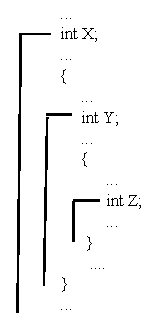
\includegraphics[width=9cm,height=6cm]{images/scope1.eps}}
\setlength{\unitlength}{1cm}
\begin{picture}(12,5.5)
\codefont{
\put(0.2,4.5){int main()\{}
\put(0.5,4.0){int numbers[10];}
\put(0.5,3.5){numbers[0] = 0;}
\put(0.5,3){numbers[1] = 1;}
\put(0.5,2.5){...}
\put(0.5,2.0){foo(numbers);}
\put(0.5,1.5){...}
\put(0.2,1.0){\}}
}
%\put(4.1,3.6){\vector(1,0){5.5}}
%\put(4.2,4.8){The box for \codefont{x} is \emph{shared} with}
%\put(4.2,4.2){\codefont{z} when the function is called.}
\put(5.8,4.3){\codefont{\large\textbf{numbers \hspace*{0.5cm}z}}}
\put(5,3.8){\codefont{numbers[0]} \hspace{0.4cm}1 \hspace{0.34cm}\codefont{z[0]}}
\put(5,3.3){\codefont{numbers[1]} \hspace{0.4cm}2 \hspace{0.34cm}\codefont{z[1]}}
\put(5,2.8){\codefont{numbers[2]} \hspace{0.4cm}88 \hspace{0.18cm}\codefont{z[2]}}
\put(5,2.3){\codefont{numbers[3]} \hspace{0.4cm}4 \hspace{0.34cm}\codefont{z[3]}}
\put(6,1.8){... \hspace{0.8cm} ...}
\put(5,1.25){\codefont{numbers[9]} \hspace{0.4cm}9 \hspace{0.34cm}\codefont{z[9]}}

\put(4.2,2.75){\codefont{.}}
\put(4.2,2.55){\codefont{.}}
\put(4.2,2.35){\codefont{.}}

\put(0,0){\large\textbf{main() and its variables}}
% ----------------  func
\codefont{
\put(11.0,4.5){int foo(int z[])\{}
%\put(11.8,4.0){int a;}
%\put(11.8,3.5){a = z + 5;}
\put(11.5,4.0){...}
\put(11.5,3.5){z[2] = 88;}
\put(11.5,3.0){...}
%\put(11.8,1.5){return a;}
\put(11.0,1.0){\}}
}
\put(10.5,0){\large{\textbf{foo() and its variables}}}

\color{\mycolor}{
\put(7.0,4.18){\line(1,0){1}}
\put(7,3.7){\line(1,0){1}}
\put(7,3.2){\line(1,0){1}}
\put(7,2.7){\line(1,0){1}}
\put(7,2.2){\line(1,0){1}}
\put(7,1.7){\line(1,0){1}}
\put(7,1.2){\line(1,0){1}}

\put(11.3,3.5){\vector(-4,-1){2.1}}
\put(13.25,5.38){\vector(1,-1){0.5}}
\put(3.7,3.55){\vector(4,1){1.2}}
\put(3.7,3.05){\vector(4,1){1.2}}
\put(8,4.18){\line(0,-1){3}}
\put(7,4.18){\line(0,-1){3}}
}
\end{picture}
\caption{Arrays are always passed to functions via pass-by-reference, so the array is ``shared'' between the two functions.  The array is named \codefont{numbers[]} in \codefont{main()} and named \codefont{z[]} in \codefont{foo()}.  Any changes made in the called function ``persist'' in the calling function. So, in this example \cf{z[2]} becomes $88$ in \cf{main()} after the function is called.}
\label{fig:arrayarguments}
\end{figure}

Arrays can be passed to functions as arguments.  
Square brackets [] denote that a function's parameter is an array.  For example, lines 21 and 1c show the syntax for the function declaration (or prototype) and function definition of the \codefont{read\_board()} function, whose parameter is an array of square objects.  However, when an array is passed to the function, the square brackets are not used.  For example, when the array \codefont{the\_board} is passed to the function \codefont{read\_board()} (line 6b) there are no square brackets on the variable name.

C++ takes an important shortcut in passing an array to a function.  It does \emph{not} copy the whole array into the function; instead, it passes the address of the beginning of the array to the function.  This address \emph{references} the location of the array in memory.  Thus, when an array is passed to a function as an argument, it is passed using \emph{pass-by-reference}.  
Figure~\ref{fig:arrayarguments} illustrates this idea.

As with other pass-by-reference arguments, the result of this approach is that the function has direct access to the original data in the array.  Any changes that the function makes to the array will still exist after the function exits.

Finally, it is important to realize that in general, functions won't ``know'' how large an array is.  To overcome this limitation, the size of an array is often passed to the function as a second argument.  That is, a function is passed both an array and an integer denoting the size of the array.  Alternatively a program may use a \emph{global} variable to define the size of an array.  Global variables (described in detail next) are variables that have global\index{global}\index{variables!global} scope and therefore can be accessed by any function in a program without needing to be passed to the function as an argument.  


\subsection{Globals}
A global is simply a variable or constant that is declared before and outside of any function (including the \codefont{main()} function).
According to the rules of scope, this means that its scope extends throughout the entire program.  The variable can be accessed from within any function -- it is global.  

The most common use for globals is to declare a constant value that should be used throughout a program.  For example, imagine a program for calculating the area of different curved shapes.  The value of $\pi$ used (e.g., 3.141 versus 3.141592) could make an important difference in the calculated answers.  If difference functions in the program used different values of $\pi$ the program might produce confusing or nonsensical results.  Creating a single, global variable that stored the value of $\pi$ to be used everywhere in the program would solve this problem.  Making the variable a constant would keep the value from ever changing.

The key word \cf{const} (short for \emph{const}ant) is used to declare a constant.  Once a constant is created, trying to give it a new value anywhere in the program will cause a compiler error. 

 In the Generic Game program length of the game board (\codefont{board\_length}, declared on line 24) is a global, so any function in the game knows the length of the board.  Not only does this avoid errors, it also makes it simple to change the length of the board, simply by changing the variable's value.

\subsection{Characters}

The \codefont{char}\index{character}\index{char@{\cf{char}}}\index{type!char@{\cf{char}}} type (short for character) holds a single character; for example `a', `b', `6', `]', or `.'.  Characters are denoted by single quotes.  Thus,
\codefont{`a'} represents the \emph{character} a; \codefont{a} represents a \emph{variable} named \cf{a}; and \codefont{``a''} is a \emph{string} containing the single character a.   Characters are stored in memory as integers, with each character represented by its own \emph{ASCII}\index{ASCII} value.\footnote{ASCII stands for American Standard Code for Information Interchange.}  For example, the character \codefont{`a'} has the value 97 and the character \codefont{`\#'} has the value 35.  Nonprinting characters like escape and tab also have ASCII values that allow them to be treated as characters.  Because each character has a unique numeric value, characters can be used as \codefont{case} values in a switch statement.  For example,\\
\codefont{
case `a':\\
}
is legal as part of a switch construct, which makes it simple to create menus with character, rather than numeric, options.

\section{Analysis of the Code}

\mysubsubsection{Lines 1-6: \#includes}

As in the previous programs these are preprocessor commands that include additional libraries.  

\mysubsubsection{Lines 8-18: The \cf{Square} Class Declaration}

Lines 8-18 are the declaration of the \cf{square} class.  The class structure is the same as for the \cf{pet} class in the previous project.  The class consists of data members and member functions.  As is common in classes, the data members are private and the member functions are public.  Thus, the only way to change or use the data within an object of type \cf{square} is to use one of the public member functions.  Each square on the game board is represented by one object of type \cf{square}.  So, for a board with 20 squares, 20 objects of type square will need to be created (this is done by creating an \emph{array} of \cf{square} objects, described below).

Each object of type \cf{square} has three data members:
\begin{tight_enumerate}
\item \codefont{move} - This is an integer that stores the distance that a player moves forward or backward after landing on the square.  For example, if a player lands on a square whose \codefont{move} value is -2, they move backwards 2 squares.  For most squares, \cf{move} is 0; nothing special happens.
\item\codefont{message} - This is a string that stores the message that's printed when a player lands on the square.  For most squares, it is blank; there is no special message.
\item\codefont{symbol} - This is a character that stores the symbol/character that is printed on the screen for the square.  A special square (with a nonzero move and a nonblank message) might be printed on the screen as a `?'.  For most squares, the symbol is a space; there is no special symbol.
\end{tight_enumerate}

There are four member functions that can be applied to each object of type \cf{square}:
\begin{tight_enumerate}
\item \codefont{square()} - This is the constructor.  It's called when a new object of type \cf{square} is created.
\item \codefont{print()} - This function `prints' a square -- that is, it prints some of the data associated with an object of type \cf{square}.
\item \codefont{action()} - This function returns the amount that a player should move forward or backward after landing on a square.
\item \codefont{set()} - This function is used to ``set'' the data of an object of type \cf{square}.  The function takes three arguments, corresponding to a square object's three data members.
\end{tight_enumerate}

\mysubsubsection{Lines 20-22: Function Prototypes}

Lines 20-22 define the prototypes for the three functions that are part of the project.  Notice that the program contains both member functions of the square class (lines 14-17) and general functions that are not associated with any class (lines 20-22).  

\mysubsubsection{Line 24: Global  Constant}\index{constant}\index{global}\index{variables!constant}\index{variables!global}

Line 24 defines a \emph{global}, \emph{constant}: \codefont{board\_length}.  The keyword \codefont{const}\index{const} makes the variable a constant, meaning that the value, once set, cannot be changed anywhere else in the code.  Constants are useful for storing values that shouldn't change, values like $\pi$ or the gravitational constant \emph{g}, or in this case, the length of the game board.

The variable \codefont{board\_length} is a global because it is declared before \cf{main()}.  Following the rules of scope (discussed in Chapter 3), this means that the scope of \codefont{board\_length} extends throughout the entire program, including \codefont{main()}, the other functions, and the class.  

\mysubsubsection{Line 4b: Array Declaration}

Line 4b declares an \emph{array} of variables of type \cf{square}.  The array is named \codefont{the\_board}.  The square brackets make this an array declaration, and the value \codefont{board\_length} within the brackets means that the array is \codefont{board\_length} items long.   So, line 4b creates an array of \codefont{board\_length} objects of type \cf{square}.  This array represents the game board (hence the name \codefont{the\_board}).  The $N^{th}$ square on the board (or the $N^{th}$ element of the array) can be accessed by the statement \codefont{the\_board[N]}, but remember that array elements are numbered starting from 0.

\mysubsubsection{Line 5b: Random Seed}
This sets the random seed to be equal to the current time.  This should result in a unique sequence of rolls each time the game is played.

\mysubsubsection{Lines 6b and 1c-13c: The read\_board() Function}\index{files!read}\index{ifstream@{\cf{ifstream}}}\index{libraries!fstream@{\cf{ifstream}}}\index{fstream@{\cf{fstream}}}

The \codefont{read\_board()} function reads a number of data items out of the file ``game.txt'' and stores them in an array of objects of type \cf{square}.   It sets up the special squares on the board.  

Line 6b simply calls the \codefont{read\_board()} function, which is defined on lines 1c-13c.   The return type for the function is void -- it doesn't return anything.  The parameter of the function is \codefont{square b[]}.  This means that the function should receive an \emph{array} (because of the brackets \cf{[]}) of square objects and will, within the function, name the array \codefont{b}.  

Line 2c creates a new variable named \codefont{infile} of type ifstream.  Line 3c uses the \codefont{open()} member function to open the file \codefont{game.txt}. 

Lines 4c-6c declare variables that will be used within the \codefont{read\_board()} function. 

Lines 7c and 12c define a \codefont{while} loop. The condition for the loop is:
\codefont{!infile.eof()}\\
The command \codefont{infile.eof()} calls the function \codefont{eof()}, which is a member function of the class \codefont{fstream} (note the use of the dot notation for a member function of a class).  The function name, \codefont{eof()}\index{eof@{\cf{eof()}}}\index{files!eof@{\cf{eof()}}}, is short for ``End Of File.''  The function \cf{eof()} returns the Boolean value \codefont{true} if the end of the file is reached and \codefont{false} otherwise.  The ! symbol is the Boolean \emph{NOT}.  Thus, line 7c can be read as:
\emph{while infile is not at the end of the file, execute the code in the loop}.

Lines 8c and 9c read data out of the file called ``game.txt'' that was opened on line 3c, and store the data in local variables.  Lines 8c and 9c use notation similar to that used with \codefont{cin}, except that instead of reading data from the keyboard, the data is read from a file.  

Line 9c calls the \codefont{getline()} function, which is defined in the iostream library.  The function \cf{getline()} is a member function of the \cf{ifstream} class, so the dot notation is used.  The function takes a \emph{source} (in this case the variable \codefont{infile}, which is connected to the file ``game.txt'') and reads a string of characters, stopping when it reaches a newline ($\backslash n$) character.  The string is then stored in the second argument to the \codefont{getline()} function, which, in this case is \codefont{square\_message}.

Line 1d in the Listing~\ref{listing:game.txt} is the first line of the \codefont{game.txt} file.  So, after lines 8c and 9c are executed, the program should store the following:\\
\codefont{square\_number = 7}\\
\codefont{square\_move = -2}\\
\codefont{square\_symbol = `?'}\\
\codefont{square\_message = ``Go back 2 squares.''}\\

Finally, line 10c checks that the \codefont{square\_number} is within the bounds of the array.  If it is, line 11c takes the last three values and passes them to the \codefont{set()} member function of object number \codefont{square\_number} of the array \codefont{b[]}.  Recall that \codefont{b[]} is an array of objects of type \cf{square}.  Thus, in the first part of line 11c: \codefont{b[square\_number]}, refers to one of the objects in this array.  The rest of line 11c, \codefont{.set(square\_move,square\_symbol,square\_message)}, calls the \codefont{set()} function of the class \cf{square} and passes three values in as arguments.  The \codefont{set()} function stores the data it receives in the square object's data members.  

Because all of the data is read from a file, it is not necessary to change \emph{any} of the code to change the board.   The board can be completely changed simply by modifying the file ``game.txt.''

\mysubsubsection{Lines 7b, 8b, 26b, 27b, and 14c-25c: The print\_board() Function}

The \codefont{print\_board()} function prints the game board for one player.  To print the board for both players it gets called twice.  It's called twice on lines 7b and 8b to print the board the first time, and on lines 26b and 27b to print the board after each player's turn.  It prints the board by stepping through each element in the array of squares and either printing the square or, if a player is in the square, prints the player's number.

The \codefont{print\_board()} function is defined starting on line 14c.
The function doesn't return any values, so the return type is \codefont{void}.  It takes three arguments: the first is an array of objects of type \cf{square} (the board), the second is an integer storing the current player's position, and the third is an integer storing the current player's number.

Lines 15c and 20c use a new type of loop, the \codefont{for}\index{for loop@{\cf{for} loop}}\index{loops!for@{\cf{for}}} loop.  A \codefont{for} loop loops for a set number of steps, typically using a counter variable to count how many steps the loop has gone through.  In this case, the loop command is:\\
\codefont{for(int i = 0; i < board\_length; i++)}\\
When the loop is first entered, it executes the \codefont{int i = 0;} command, which creates a new variable \codefont{i} and sets its value to 0.  Next, the loop checks the condition \codefont{i $<$ board\_length}.  If it is true, the code within the loop is executed; if it is false, the loop is skipped (the program jumps to line 21c).  Because \codefont{i} is initially 0 and \codefont{board\_length} is 20 (line 24)  the loop is executed.  When the end of the loop is reached, at line 25c, execution returns to the beginning of the loop and the command \codefont{i++} is executed.  This increases \codefont{i} by 1.  Then the condition is checked again.  If it is still true, the code within the loop is executed again; if it has become false, the loop is skipped.  

\begin{wrapfigure}{R}{0.5\textwidth} \framebox[\linewidth][l]{\parbox{0.95\linewidth}{\codefont{Arrays and \cf{for} Loops} \\
Because arrays generally have to be accessed one element at a time, they are often used in conjunction with \cf{for} loops.  For example, the code\\
\codefont{
for(int i =0; i < array\_length; i++)\\
\hspace*{0.5cm}b[i] = a[i];\\}
will copy the values of array \codefont{a} correctly into array \codefont{b}.  The statement
\codefont{b = a;} will \emph{not} copy the array elements.  

Similarly, to print all of the elements of an array, the code\\
\codefont{
for(int i =0; i < array\_length; i++)\\
\hspace*{0.5cm}cout << a[i] << endl;\\}
will work, but\\
\codefont{cout << a;} will \emph{not} print the array elements.
}}
\vspace{-0.5cm}
\end{wrapfigure}

Thus, in the loop defined on lines 15c and 20c, the loop counter \cf{i} starts at 0, each time through the \codefont{for} loop, \codefont{i} increases by 1 until it is no longer less than \codefont{board\_length}, at which point the loop is exited.  The \codefont{for} loop counts from 0 to the length of the board and either prints what appears in each square on the board (line 17c) or prints the player's number (line 19c).

During each iteration of the loop, the \codefont{if} statement on Line 16c checks whether this is \emph{not} the player's current position (i.e., whether \codefont{i} is not equal to \codefont{player\_position}).  If it is not the player's position, it calls the \codefont{print()} function on object \codefont{b[i]} -- the \emph{i}th element in the array \codefont{b}.  This happens on line 17c:\\
\codefont{b[i].print();}\\
where \codefont{b} is the array of square objects corresponding to the game board, \codefont{i} is the current square on the board (the one being printed), and the \codefont{print()} function is a member function of the \cf{square} class.  So, this command ``asks'' the \emph{i}th square object of the array \codefont{b} to print itself.  (The \codefont{print()} member function of the square class is described below.)

If the current value of \codefont{i} \emph{is} equal to the player's position, then the player's number is printed instead (line 19c).  

Line 21c prints the word ``goal,'' marking the end of the board.

Lines 22c and 23c define a second \cf{for} loop.  This one prints a series of hyphens to denote the middle of the board.  Finally, line 24c adds a last new line to make the output cleaner, and the function returns from the final closing bracket on line 25c.

Note that the \codefont{print\_board()} function is called on both line 7b and line 8b.  The first time it is called, the arguments are \codefont{the\_board}, \codefont{player1\_position}, and the number 1.  So, the function prints the board and places a 1 in player 1's position.  The second time it is called, the arguments are \codefont{the\_board}, \codefont{player2\_position}, and the number 2.  So, the function prints the board and places a 2 in player 2's position.  

\mysubsubsection{Lines 9b-29b: The Game Loop}

Lines 9b and 29b define the main game loop.  It is quite similar to the game loop used for NIM in Chapter 2, except that the condition for continuing the loop is:\\
\codefont{((player1\_position < board\_length - 1) \&\& (player2\_position < board\_length-1))}.\\
The program will continue the loop when: 
\emph{player 1's position is less than the board length-1 AND player 2's position is less than the board length-1}\index{AND@{\cf{AND}}}\index{Boolean!AND@{\cf{AND}}}.
 The symbols, \&\&, define the Boolean AND, which is true only if \emph{both} arguments are true.  So if player 1 hasn't reached the end of the board and player 2 hasn't reached the end of the board, the program will loop, continuing the game. 

The $-1$ is included in the test conditions because the board (being an array) starts at 0.  So, the last square on a twenty square board is square number nineteen. 

%Note that the symbols \&\& stand for the Boolean AND operation.  Also, recall that in an array with $N$ elements the elements are numbered from 0 to $N-1$, so the actual board squares are also numbered from 0 to \codefont{board\_length-1} and so play continues until one of the players reaches the \codefont{board\_length} - 1 square.

\mysubsubsection{Lines 10b-13b: Player Move}
Line 10b is just output telling the current player to press Enter to roll. Line 11b ignores any input, but still waits for the Enter key to be pressed.  Without it (try commenting it out), the game zips by in a flash.  Line 12b generates the player's actual roll, following the same general form as the random move in NIM.  
%In this case the modulus operation (the \% operator) returns a number between 0 and 4 because any random number divided by 5 gives a remainder between 0 and 4 and then adds 1 to it to give a roll between 1 and 5.  Of course, these can be changed to make the rolls in any range the programmer likes.  Finally 
Line 13b prints the roll.  %This is not necessary for the functioning of the program as the player's `piece' is moved automatically, but the player should know what they rolled rather than having to count backwards to figure it out.

\mysubsubsection{Lines 14b-25b: The Move} 

Lines 14b, 20b, 21b, and 25b define an if-else structure used to make sure that the correct player gets to move.  Lines 15b and 21b add the current roll to the current player's position using the \codefont{+=} operator.


\begin{wrapfigure}{R}{0.5\textwidth} \framebox[\linewidth][l]{\parbox{0.95\linewidth}{\codefont{Curly Braces (\{\}'s) or No Curly Braces} \\
In the previous programs, curly braces (\{\}'s) were used to denote blocks of code within if-else statements and loops, but the if-else statement on lines 16c-20c do not use curly braces.  This works because there is only one line of code for the if condition and one line of code for the else condition.  Curly braces are only \emph{required} when the condition applies to more than one line of code.  However, curly braces can always be included, even if they only surround one line of code.  In general, including braces is a good idea,  they are omitted here to save space.  The same rules apply to loops that include only one line of code; for example, lines 22c and 23c.
}}
\vspace{-0.5cm}
\end{wrapfigure}

 Lines 16b and 22b call the \codefont{check\_position()} function.
A lucky (or unlucky) roll or square could send the player beyond the bounds of the board.  So, the \codefont{check\_position()} function is necessary to check whether the player's position is less than 0 (line 27c) or greater than the board length (line 29c), and to correct the player's position if it has exceeded the bounds of the board.
The \codefont{check\_position()} function is called each time a player's position is changed. 
The test conditions are less than 0 or greater than \codefont{board\_length-1} because as an array, the board squares are numbered from 0 to \codefont{board\_length-1}.

The function uses a pass-by-reference parameter.  Instead of returning the new position, the function simply changes the argument's value (line 28c or 30c).  However, because the parameter \codefont{p} is pass-by-reference, as determined by the \& symbol in function declaration (line 22) and the function definition (line 26c), the change made to \codefont{p} in the function changes the \codefont{player1\_position} or \codefont{player2\_position} variable that was passed into the function (lines 16b, 18b, 22b, and 24b).

After the player's roll has been added to their position and his or her position has been checked against the length of the board, and corrected if necessary, the board array is checked to see if anything special happens in the square the player landed in.  This is done on line 17b or line 23b, with the statement:\\
\codefont{player1\_position += the\_board[player1\_position].action();}\\
The \cf{+=} operator is used to change the value of the player's position by the amount \emph{returned} by the function call: \codefont{the\_board[player1\_position].action();}

Then \codefont{the\_board[player1\_position]} is the square object corresponding to the location of the player.  For example, if player 1 is at position (or square) 3, then the variable \codefont{player1\_position} holds the value \codefont{3} and therefore \codefont{the\_board[player1\_position]} refers to square 3.  The next part of the command \codefont{.action()} calls the member function \codefont{action()} for that particular square.  

The \codefont{action()} member function is described in detail next.  For now, it's sufficient to know that it prints the message associated with the square (e.g., ``Bad winds, go back three squares'') and returns the distance the player moves (e.g., -3).  In the initial version of the game most squares have no effect and don't print any message.  

After the player's position has been updated to reflect the action, if any, for the square he or she landed in (line 17b or line 23b), the position is checked again to make sure that the player is still within the bounds of the board.  (This isn't necessary if the programmer is careful with actions; for example, no action sends a player who lands on square 2 back 7 squares.  However, it is good programming practice to have the program double-check because the person rewriting the game file may not understand the details of the game.)  

After the player has been moved by an action, the new square is \emph{not} checked for another action.  So, if a player lands on a square that sends him or her back 3 squares and the new square landed on would send him or her forward 4 squares, the player doesn't go forward 4 squares.  This can be changed, but the current approach avoids the possibility of the player getting caught in an infinite loop of ``go forward 2'' ``go back 2.'' 

\mysubsubsection{Lines 26b-27b: Reprinting the Board}

Lines 26b and 27b simply reprint the board with the new player positions by calling the \codefont{print\_board()} function.

\mysubsubsection{Line 28b: Next Player's Move}

Line 28b changes the current player from 1 to 2 or vice versa, similar to how it was done in NIM.

\mysubsubsection{Lines 30b-33b: The End of the Game}

If the program breaks out of the \cf{do-while} loop on lines 9b-29b, it's because one of the players has reached the end of the board, making the condition on line 29b false.  Line 30b changes the current player \emph{back} to the winner (the current player was changed on line 28b, so the identity of the winner has to be changed back).  Line 31b prints the winner message.  Line 32b pauses and waits for the user to hit Enter.  

\subsection{Lines 33c-49c: The \cf{Square} Class Definitions}

This section details the member functions of the \cf{square} class: \codefont{square()}, \codefont{action()}, \codefont{print()}, and \codefont{set()}.  These are all very short functions, but are useful for keeping the data about the squares of the board separate from the rest of the program.  The text \codefont{square::} in the function definitions indicates that these functions are members of the \cf{square} class and not stand alone functions like \codefont{read\_board()}, \codefont{print\_board()}, and \codefont{check\_position()}.

\mysubsubsection{Lines 33c-37c: The \cf{square()} Function (the constructor)}

The function \codefont{square()} is the constructor for the \cf{square} class.  It is called whenever a new object of type \cf{square} is called.  It sets the initial values of an object of type \cf{square}, setting the \codefont{symbol} to a space (line 34c), the \codefont{move} to 0 (line 35c), and the \codefont{message} to ``'', that is, no message, (line 36c).  These are the default values for ``normal'' squares on the board.

For the special board squares these values are changed by the \codefont{read\_board()} function (lines 1c-13c) calling the \codefont{set()} function (lines 45c-49c, described below).

\mysubsubsection{Lines 38c-41c: The \cf{action()} Function}

The \codefont{action()} function is called when a player lands on a square.  Line 39c prints the message associated with the square (e.g., ``Bad winds, go back 3 squares'' for special squares, or a blank message ``'' for normal squares).  Line 40c returns the amount that the player is forced to move by the square (e.g., -3).  This return value is used to adjust the player's position on line 17b or line 23b, depending on whose turn it is.

\mysubsubsection{Lines 42c-44c: The \cf{print()} Function}

The \codefont{print()} member function prints the symbol associated with a square; for example, a blank for normal squares and a special symbol like `?' or `*' for special squares.  The function is called by the \codefont{print\_board()} function.

\mysubsubsection{Lines 45c-49c: The \cf{set()} Function}

The \codefont{set()} member function is used to set the data that a square object holds.  When a new square is created, the constructor sets all of its data to the default values: no action, no message, and a space for a symbol.  The \codefont{set()} member function is used by the \codefont{read\_board()} function to change these values for special squares (line 11c).

\subsection{The Data File}

Listing~\ref{listing:game.txt} is the data file, called ``game.txt'' and used to define the board.  The data file is opened and read by the \codefont{read\_board()} function.  This function expects to find very specific data in a very specific order:
\begin{tight_itemize}
\item An integer - This is the number of the special square to be added to the board. It should be between 0 and \codefont{board\_length-1}.
\item A character - This is the symbol to be printed on the board for the special square.
\item An integer - This is the amount a player is moved if he or she lands on the square (negative numbers for backward moves).
\item A string - This is the message to be printed if the player lands on the special square.
\end{tight_itemize}
For example, line 1d in the file is:\\
\codefont{7 -2 ? Go back 2 squares.}\\
which means square number 7 is special (this is actually the eighth square because the array starts  at zero).  It is printed on the board with a ?.  If a player lands on it, the message ``Go back 3 squares'' is printed, and they go back 2 squares (-2).  

The \emph{mechanics} of the game are defined by the program: how many players there are, who moves when, what the rolls are, etc.  However, the details of the game (which squares are special, what effects they have, and what messages are printed) are defined by the data file.  A completely different flavor of game, with different special squares and different messages, can be created simply by rewriting the data file ``game.txt'' without changing any of the code.  

\vspace{+0.25cm}
{\color{\mycolor}\noindent\hrulefill}
\section{Exercises: Modifying the Program}

The current game is very simple and not particularly interesting to play.  Changing the output and the game file would make the game more interesting.  In addition, there are ways to change the game to make it more of a challenge to the players.  

\mysubsubsection{Exercise 1: Customize the Game}
Rewrite the ``game.txt'' file to customize the game.  First, pick a theme: a sailing game, a car racing game, an ``escape the zombies'' game, a ``kill all humans'' game, etc..  Then change the ``game.txt'' file, particularly the messages, to fit the theme.  Add more lines to the data file to make more squares on the board special.  It's a good idea to test each addition or change to the game file individually.  It's very frustrating to add 15 new lines and then have to figure out which of the new lines contains the typo that keeps the file from being read correctly.

\mysubsubsection{Exercise 2: Add an Introduction}
Add an introduction to the game that sets the stage and explains the rules.  For example, if your game is a zombie apocalypse game, add an introduction describing how the zombie's arose and the players' goals.    \\
{\bf Challenge:} Add the introduction to the beginning of the ``game.txt'' file and have the program read and print it.  This is important if you want the same program to be able to read and play different game files.

\mysubsubsection{Exercise 3: Improve the Output}
Change how many blank lines are added between moves to make it clearer how the players are moving along the board.  Then change the \codefont{print\_board()} function to vary how the board itself is drawn.  Add vertical bars ($|$'s)  between each square to make the board look more like a series of separate squares, or add a row of hyphens above the board.

\mysubsubsection{Exercise 4: Players' ``Pieces''}
Currently the players appear on the board as a 1 and a 2.  Change the game so that they appear as different characters and to allow each player to pick his or her own symbol.  This will require some extra code at the beginning of the game asking the player what symbol is wanted and two new variables of type \codefont{char} to store those symbols.

\mysubsubsection{Exercise 5: Other changes}
There are a lot of other simple changes that can be made to the game.  Change the length of the board.   Notice how much harder it would be to change the length of the board if instead of the global constant \codefont{board\_length}, the actual number 20 (or 19) was used everywhere.  It would be necessary to find and change every instance of the value, instead of just making one change to the constant.  Then change the range of allowed rolls.  Try changing the game so that negative rolls are possible; for example, players can roll any value from -1 to 4. 

\mysubsubsection{Exercise 6:  Multi-player}
Change the game so three or more players can play.  Then change the game so that the user can decide how many players there will be (up to some limit).  There needs to be a new variable to keep track of the total number of players.  The value of the variable should be set by the user at the beginning of a game.  Then this value is used as part of the modulus operation on lines 28b and 30b to decide who goes next.  To print the board, it will probably be necessary to add a \cf{for} loop that loops over the number of players, calling \codefont{print\_board()} once for each player.  Finally, the if-else statement on lines 14b-25b probably needs to be replaced with a switch statement based on the \codefont{current\_player}.

\section{Problems}
The potential for modifying the generic game should now be clear.  There are also more complicated changes that can be made to the overall game mechanics.
\begin{enumerate}[{\bf 1.}]

\item {\bf Many games in one}\\
 Currently, the program always reads the game data from the file ``game.txt,'' which means the program always plays the same game.  Have the program ask the user (e.g., in the \codefont{read\_board()} function), which file to open (or which game to play) and then open the appropriate file.  This will allow the user to choose between games (e.g., sailing or escape the zombies), when the program starts.

\item {\bf Random squares}\\
 Instead of always moving the same number of squares, make special squares move the player by a random amount.  The \cf{action()} function will need to be changed to generate a random action instead of always returning the same value.  
In addition, the ``game.txt'' file, the \codefont{read\_board()} function, and the \cf{square} class will need to be rewritten so that there is a way to indicate and remember whether a special square should be a random square or a deterministic square.  One approach is to use two integers in the ``game.txt'' file to set the upper and lower limits of a random move.  If the two bounds are the same (e.g., -3 and -3), then the move is deterministic.

\item {\bf More complex squares}\\
 Add a type of square that has a more complex effect.  For example, a square that allows the player to take another roll or squares that force the player to miss a turn.  As in the previous problem this will probably require changing the ``game.txt'' file, the \codefont{read\_board()} function, and the \cf{square} class so that the new square types can be correctly read from the data file and stored in the square objects.

\item {\bf Additional game variables}\\
 Have players start with some gold (or health or fame, etc.).  As the game progresses, special squares cause each player's gold (or health, etc.) to increase and decrease.  Change the victory conditions to match the new variable.  For example, the game might end when the first player reached the goal, but the winner is the player with the most gold (and maybe the first player to reach the goal gets some bonus gold making it more likely that the player will win).  Make sure that the game's introduction, instructions, and comments accurately explain the new version.

\item {\bf Player choices}\\
One limitation of the game is that it's completely random; there's no element of skill.  Fix this by giving the players' options.  Allow players to choose between moving two squares ahead (slow, but sure) or rolling to move a random amount (say from 1 to 4).  Which choice is more strategic would depend on what squares are ahead (does the player want to try to jump over an unlucky square?) and how far ahead or behind he or she (a player who was already way ahead might take the slow, but steady option, whereas a lagging player might hope to get lucky and catch up).

\item {\bf Squares with choices}\\
Create a new type of square that gives the player an option.  For example, a square where the player who lands on it either goes back three squares OR gives the opponent a +1 bonus on his or her next roll.  This requires a more complex ``game.txt'' file to denote these special squares and both the ability to read the file and store the information in the \cf{square} class.\\
{\bf Challenge:} Invent at least two more types of special squares that give the player an option and include them in your game. In some cases both options could be beneficial.   Possible options for a player to choose from could include, going backwards $N$ squares, losing a turn, sending an opponent forwards, getting an extra roll, getting a bonus on the next roll, etc.

\end{enumerate}

\addtocounter{interlude}{1}
\setcounter{section}{0}
\setcounter{figure}{0}
%********** Interlude **********
\interlude{C++ Compared to C}
\addtocounter{chapter}{-1}
Although C++ is widely used, C (the precursor to C++) remains a very important language.  C is a particularly good language when there is a need to optimize speed and memory use.  Thus, in addition to ``regular'' applications, C is often used for programming microcontrollers, embedded computers, and other small-scale computing devices.  This makes the ability to program in C  a very useful and marketable skill.  

 C++ is an extension of C and was designed to be backwards compatible with C, so any C program can be compiled by a C++ compiler (although not vice versa).  Learning the differences between the two languages, particularly what features of C++ are not available in C and what C uses instead, grants many of the benefits of knowing two programming languages, without having to learn two complete languages.

The major difference between C++ and C is that C does not support classes.  Instead, C uses a similar, but more ``primitive,'' data entity known as a \emph{structure}\index{structure} (which was introduced in Interlude 3).  Because C does not support classes, code that depends upon classes is also not supported, most notably the \codefont{iostream} and \codefont{fstream} libraries and the \codefont{string} class.  C has a separate set of input and output functions instead of those defined in the \codefont{iostream} and \codefont{fstream} libraries, and C has a separate structure, C-style strings, instead of C++'s \codefont{string} class.  To maintain backward compatibility, all of these elements of C are legal in C++ code as well.

\section{Structures}

Because C does not support classes, any program that depends on or uses classes cannot be a C program.   Thus, the \codefont{pet} class used in the Electronic Pet project and the  \codefont{square} class used in the Generic Board Game program cannot be created or used in C.  

Instead of classes C uses structures that are defined using the keyword \codefont{struct}\index{struct} (see Interlude 3).  Like classes, C structures can contain multiple data members.  However, structures don't have function members.  Instead functions can be written to accept structures as arguments or to return structures.  

For example, in C a \codefont{pet} structure would be defined:\\
\codefont{
typedef struct pet\{\\
\hspace*{0.5cm} int happy;\\
\hspace*{0.5cm} int hunger;\\
\hspace*{0.5cm} char name[100];\\
\} pet;\\
}
Note that with this definition, a \codefont{pet} structure has the equivalent of three data members: two integers (\codefont{happy} and \codefont{hunger}) and an array of characters (\codefont{name}).  There are no member functions, although functions can be written to accept structures as arguments or to return structures.   Because strings are not supported in C, an array of characters (characters were introduced in Chapter 6) is used to store pets' names.  These character arrays are known as a C-style strings and are described below.

Once a structure has been defined, it can be used very much like any other type.  Variables can be declared:\\
\codefont{pet pet1, pet2;}\\
and functions can both accept structures as arguments and can return them:\\
\codefont{pet function(pet p, pet p2)}\\
The ``data members'' of a structure are accessed using the same dot notation as class members:\\
\codefont{pet1.hunger = 50;\\
pet1.happy = 50;\\
}
but all of the data is public.

Thus, to change the \codefont{pet} class in the Electronic Pet program into a C-style structure, two major changes are necessary.  First, the class declaration have to be changed into a structure containing only the data elements.  Second, all of the member function definitions have to be rewritten as nonmember functions with \codefont{pet} structures as parameters.

For example, the \cf{print()} function from the pet class would be rewritten to take a pet structure as an argument and then would print its data members:\\
\cf{
void print(pet p)\{\\
\hspace*{2cm}// print p.name\\
\hspace*{2cm}// print p.hunger\\
\hspace*{2cm}...\\
\}
}
Note that the pet structure to be printed is passed in as an argument.  The dot notation is used to access and print its data members.  This new \cf{print()} function is not a member of any class.

\section{C Input and Output}

Because classes are not supported in C, neither are the \codefont{iostream} and \codefont{fstream} libraries.  Thus, the input and output classes and their associated objects and operators (\codefont{cin}, \codefont{cout}, \codefont{$<<$}, \codefont{$>>$}, etc.) are not available in C.  C has its own set of functions for input and output, the most common of which are listed in Table~\ref{tab:operators2}.

\begin{table}[h]
\centering
\caption{Common C Input and Output Functions.  These are also available in C++.}
\begin{tabular}{|  l |  p{7cm} |}
\hline
%\bold{Command} & \bold{Full Name} & \bold{Description} \\
\textbf{Function} &  \textbf{Use} \\
\hline
\codefont{printf()} & Output to the screen \\
\hline
\codefont{scanf()} & Input from the keyboard \\
\hline
\codefont{fprintf()} & Output to files \\
\hline
\codefont{fscanf()} & Input from files \\
\hline
\end{tabular}\label{tab:operators2}
\end{table}

All of the output functions use a similar format.  They are passed a single \emph{format string}\index{format string} that may include \emph{format specifiers}\index{format specifiers}, denoted by a \%, which are used to print variables.  This format string is followed by the arguments to be printed, one argument for each of the format specifiers listed in the format string.
For example, the code:\\
\codefont{
int X = 7, Y = 9, Z;\\
Z = X + Y;\\
printf("The value of \%d plus \%d is \%d.", X, Y, Z);\\
}
will print:\\
\codefont{
The value of 7 plus 9 is 16.\\
}
Each format specifier (e.g., \cf{\%d}) in the format string is replaced by the value of the corresponding variable.  For example, the value of \codefont{X} is substituted for the first format specifier, the value of \codefont{Y} for the second format specifier, etc.  The type of the argument must match the format specifier; for example, the format specifier \codefont{\%d} must be matched to an integer.  Table~\ref{tab:formatspecifiers} lists a few of the common format specifiers and their corresponding types.  A format specifier can also specify how a number is printed, for example, it's printed precision, as shown in  Table~\ref{tab:formatspecifiers}.  

The input functions are handled similarly to the output functions.  For example, the command:\\
\codefont{
scanf("\%d \%f", \&x, \&f);\\
}
reads an integer and a decimal number from the input and stores them in the variables \codefont{x} and \codefont{f}, respectively (assuming that \codefont{x} and \codefont{f} have the appropriate types -- otherwise, the compiler produces an error).  The \codefont{scanf()} expects pointers (discussed in Chapter 7), which requires that an \& be used in front of the variables: \codefont{x} and \codefont{f}, unless the variables were declared as pointers.

The functions for reading from and writing to a file are \codefont{fscanf()} and \codefont{fprintf()}.  In C++, reading from or writing to a file requires creating and using a file stream object.  In C, it requires using a pointer  (see Chapter 6) to a variable of type \codefont{FILE}. The basic code is:\\
\codefont{
FILE *openfile;\\
int f;\\
openfile = fopen("filename","r");\\
fscanf(openfile, "\%f", \&f);\\
}
The asterisk (*) in the declaration \codefont{FILE *openfile} makes \codefont{openfile} a pointer to a \codefont{FILE} (pointers are discussed in Chapter 6).  The character string \codefont{``r''} defines the \emph{mode}\index{files!mode} for opening the file.  Common modes are read (\codefont{r}), write (\codefont{w}), and append (\codefont{a}).  If the program attempts to open a file for writing or appending that does not exist the program will attempt to create the file.  


\begin{table}[h]
\centering
\caption{Common C Format Specifiers.}
\begin{tabular}{|  c  |  p{12cm} |}
\hline
%\bold{Command} & \bold{Full Name} & \bold{Description} \\
\textbf{Specifier} &  \textbf{Type and precision} \\
\hline
\codefont{\%d} & Signed integer \\
\hline
\codefont{\%f} & Floating-point number \\
\hline
\codefont{\%c} & Character \\
\hline
\codefont{\%s} & C-style string of characters \\
\hline
\codefont{\%e} & Floating-point number in scientific notation \\
\hline
\codefont{\%\%} & Prints a \% symbol \\
\hline
\codefont{\%10d} & Signed integer, with a width of 10, right-justified, and with leading blanks \\
\hline
\codefont{\%4.2f} & Floating-point number with width 4 and a printed precision of 2\\
\hline
\end{tabular}\label{tab:formatspecifiers}
\end{table}

\section{C-style Strings}\index{strings!C-style}

The lack of classes in C means that the \codefont{string} class used throughout this text is not supported in C.  The most common alternative is to use \emph{C-style strings}\index{C-style strings}.  Although the \cf{string} class has a number of useful and powerful capabilities, there are good reasons to learn to use C-style strings even for a strict C++ programmer.   First, command-line arguments (see Interlude 6) are C-style strings, not objects of the \cf{string} class.  Second, there are some applications for which C-style strings are more appropriate or easier to use than string objects.  Finally, because C-style strings are often used in C++ programs, it is useful to be able to read and understand code that uses C-style strings.

C-style strings are simply arrays of characters that are terminated by a null terminator,\footnote{Sometimes called the \emph{null character}.}\index{null terminator}\index{null character} the character `\textbackslash 0', which has the ASCII code 0.  The null terminator solves the problem of not knowing the length of a character -- the array is simply read until the null terminator is reached.  Thus, a typical piece of code to manipulate C-style strings contains a loop like:\\
\codefont{
int i = 0;\\
while(str[i] != '\textbackslash 0')\{ \\
\hspace*{0.5cm} // Do something with each character str[i]\\
\hspace*{0.5cm} i++;\\
\}\\
}
where \codefont{str} is the name of the C-style string.

When an array of characters is created and initialized, the null terminator is automatically added.  So, the statement\\
\codefont{char str[] = "string";}\\
creates an array with seven elements, with the seventh element being the null terminator.

The \codefont{cstring}\index{libraries!cstring@{\cf{cstring}}}\index{cstring@{\cf{cstring}}} library contains a number of functions that can be used to manipulate C-style strings.  Table~\ref{tab:cstrings} lists a few of the most useful ones.

\begin{table}[h]
\centering
\caption{A few of the more useful functions for manipulating C-style strings.  These are found in the \codefont{cstring} library.  The asterisks (*) in the function definitions refer to pointers, which are covered in the next chapter.  Generally, any place in the code where \codefont{char *} appears a C-style array of characters is appropriate. }
\begin{tabular}{|  c  |  p{7cm} |}
\hline
%\bold{Command} & \bold{Full Name} & \bold{Description} \\
\textbf{Function} &  \textbf{Use} \\
\hline
\codefont{char *strcpy(char *str1, char *str2)} & Copies \codefont{str2} into \codefont{str1} and returns the new string. \\
\hline
\codefont{char *strcat(char *str1, char *str2)} & Concatenates \codefont{str2} onto the end of \codefont{str1} and returns the new string.\\
\hline
\codefont{char *strncat(char *str1, char *str2, int n)} & Concatenates at most the first \codefont{n} characters from \codefont{str2} onto the end of \codefont{str1} and returns the new string.\\
\hline
\codefont{char *strchr(char *str1, char c)} & Returns a pointer to the first occurrence of \codefont{c} in \codefont{str1}, or \codefont{NULL} if there is none.\\
\hline
\end{tabular}\label{tab:cstrings}
\end{table}


\addtocounter{chapter}{1}

%\addtocounter{chapter}{1}
\setcounter{section}{0}
\setcounter{figure}{0}
%********** Chapter 6 **********
\chapter{Robot World}\index{Robot World}\index{projects!Robot World}

\section{Introduction}

This chapter presents the Robot World project, which creates a simple, simulated world of robots.  Initially, the world and the robots are fairly primitive, but the program's design makes it fairly easy to make them more complex and interesting.

This chapter reviews a number of topics from  previous chapters, most notably classes and arrays.  In addition, a number of new topics are introduced:
\begin{tight_itemize}
  \item User-defined Libraries\index{libraries!user-defined}
  \item Two-dimensional Arrays\index{arrays!two-dimensional}
  \item Pointers\index{pointers}
\end{tight_itemize}

The previous programs have all included libraries of predefined code, such as the \codefont{iostream} library.  This chapter explains how to create libraries.  Libraries are convenient for breaking a large program into more manageable pieces and make it easy to share classes and functions between programs.   This chapter demonstrates how one-dimensional, list-like arrays can be extended to two-dimensional, table-like, arrays or, more generally, to \emph{N}-dimensional arrays.  Finally, this chapter introduces pointers, a type of variable that gives more direct access to memory.

\section{The Program}

The Robot World program should be separated into three separate files: the main file (Listing~\ref{listing:robotWorldMain}), which can have any name, and two library files: ``robot.h'' (consisting of Listing~\ref{listing:roboth} followed by Listing~\ref{listing:robotcpp}) and ``world.h'' (consisting of Listings~\ref{listing:worldh} followed by Listing~\ref{listing:worldcpp}).  Note that the names of the library files are used in \cf{include} statements in the other files, so can't be changed (unless the \cf{include} statements are also changed).\footnote{Libraries are often divided into two files, a .h file containing the function and class declarations and a separate .cpp file with the code definitions.  This is important for mutually dependent libraries, but for this project we will simplify matters by using only a single library file per class.}  
%To compile the program, put the code from Listing~\ref{fig:robotWorldMain} into one file (as always, don't include the line numbers); this is the main program.  Put the code from Listings~\ref{fig:roboth} and~\ref{fig:robotcpp}, in that order, into a file named ``robot.h'' and put the code from Figures~\ref{fig:worldh} and~\ref{fig:worldcpp}, in that order, into a file named ``world.h''.
%Notice that the main program already contains the code to include these libraries (lines 5 and 6).

Compile the main program. The other files will be included automatically.  Then run the program.  To see the robots move repeatedly, press, or hold down, the Enter key.  Two robots, each represented by a `\#', move around a small world consisting of periods and hyphens.  Text at the bottom of the screen supplies information about the robots' status.  Currently, the robots move randomly and don't interact with their world.  However, the structure of the program makes this relatively easy to change.  The program runs indefinitely, so it's necessary to press \codefont{control-c} to stop it.

\begin{minipage}{\textwidth}
\begin{lstlisting}[language=C++,numbers = left,xleftmargin=4.0ex, basicstyle=\small, emph={a_world},emphstyle = \color{\mycolor},
showstringspaces=false,
caption = {The main program for the Robot World program.  The code to include the libraries containing the \codefont{robot} class and the \codefont{world} class is already part of the main program (lines 5 and 6).},
label={listing:robotWorldMain}]
     #include<iostream>
     #include<cstdlib>
     #include<ctime>
     using namespace std;
     #include"robot.h"
     #include"world.h"
     int main(){
         world a_world;
         srand(time(NULL));
        a_world.set_up();
        do{
            a_world.update();
            a_world.draw();
            cin.ignore();
        }while(1);
        return 0;
    }
\end{lstlisting}
\end{minipage}

%---------------------------------------------------------------------------------------------------------

\begin{minipage}{\textwidth}
\renewcommand*\thelstnumber{\the\value{lstnumber}a}
\begin{lstlisting}[language=C++,numbers = left,xleftmargin=4.0ex, basicstyle=\small, emph={direction,energy,ID,moved},emphstyle = \color{\mycolor},
showstringspaces=false,
caption = {The declaration of the \codefont{robot} class.  It has four private data members, three private member functions, and five public member functions.},
label={listing:roboth}]
    class robot{
       private:
          int direction;
          int energy;
          int ID;
          int moved;  
          void turnLeft();                   // a private function
          void turnRight();                  // a private function
          void forward(int &, int &);        // a private function
      public:
         robot(int);                        
         void refresh() {moved = 0;}        // an in-line function
         void draw();
         void print();
         void move(int &, int &);           // pass-by-reference arguments
   };
\end{lstlisting}
\end{minipage}

\begin{minipage}{\textwidth}
\renewcommand*\thelstnumber{\the\value{lstnumber}b}
\begin{lstlisting}[language=C++,numbers = left,xleftmargin=4.0ex, basicstyle=\small, emph={energy,direction,ID,id,x,y,moved},emphstyle = \color{\mycolor},
showstringspaces=false,
caption = {The definitions of the member functions of the \codefont{robot} class.},
label={listing:robotcpp}]
void robot::turnLeft(){
      energy--;
      direction = (direction + 3) % 4; // a left is 3 rights
}
void robot::turnRight(){
      energy--;
      direction = (direction + 1) % 4;
}
void robot::forward(int &x,int &y){
      energy -= 2;
      if(direction == 0)
           y--;    
      if(direction == 2)
           y++;    
      if(direction == 1)
           x++;    
      if(direction == 3)
           x--;    
}
robot::robot(int id){
     energy = 50;
     ID = id;
     moved = 0;
     direction = 0;
}
void robot::draw(){
     cout << "#";
}
void robot::print(){
     cout<<"ID" <<ID<<": Energy = "<<energy<< "   Direction = "<<direction;
}
void robot::move(int &x,int &y){
     if(moved == 1)
          return;
     switch(rand()%4){
     case 0:
          turnLeft();
          break;
     case 1:
          turnRight();
          break;
     case 2:
     case 3: 
          forward(x,y);
          break;
     default: 
          cout << "Error in robot move." << endl;
     }
     moved = 1;
}
\end{lstlisting}
\end{minipage}

\begin{minipage}{\textwidth}
\renewcommand*\thelstnumber{\the\value{lstnumber}c}
\begin{lstlisting}[language=C++,numbers = left,xleftmargin=4.0ex, basicstyle=\small, emph={HEIGHT,WIDTH,terrain,bots},emphstyle = \color{\mycolor},
showstringspaces=false,
caption = {The declaration of the \cf{world} class.},
label={listing:worldh}]
const int HEIGHT = 10;
const int WIDTH = 10;
class world{
   private:
      int terrain[WIDTH][HEIGHT];
      robot *bots[WIDTH][HEIGHT];
   public:
      void set_up();
      void draw();
      void update();
};
\end{lstlisting}
\end{minipage}

\subsection{Two-Dimensional Arrays}

Two-dimensional arrays are similar to the one-dimensional arrays introduced in the Generic Board Game (Chapter 6) where an array was used to store a list of \codefont{square} objects representing the game board.  Two-dimensional arrays extend the idea of a list of items to a table of items.  In a two-dimensional array, each data item is referred to by its row and column number.
Two sets of square brackets are used to declare two-dimensional arrays and to access their elements.    For example,\\
\codefont{int sample\_array[5][10];}\\
declares a 5 by 10 array of integers.  Element \codefont{i,j} is accessed by the statement:\\
 \codefont{sample\_array[i][j]}\\
This pattern extends to $N$ sets of brackets for $N$-dimensional arrays.  

Because memory is simply one long list, a \codefont{X} by \codefont{Y} array is stored in memory as \codefont{X}  arrays, each of length \codefont{Y}.  To access element \codefont{i,j} of an \codefont{X} by \codefont{Y} array a program starts at the beginning of the array and moves \codefont{i*Y + j} elements ahead.   This means that if an $N$-dimensional array is going to be passed to a function, the function must be given all of the dimensions except the first.  That is the function must be declared like\\
 \codefont{return\_type function\_name(argument\_type array[][Y])}\\
where \codefont{Y} is the size of the array's second dimension.  The size of the first dimension can be included, but it doesn't have to be.  For \codefont{N} dimensional arrays passed as arguments to functions, the size of the last \codefont{N - 1} dimensions must be given.




\begin{figure}
%\centerline{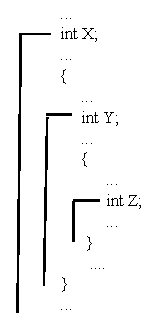
\includegraphics[width=9cm,height=6cm]{images/scope1.eps}}
\setlength{\unitlength}{1cm}
\begin{picture}(10,3)
\linethickness{0.3mm}

\put(2.3,2.5){\codefont{ptr}}

\put(4.3,2.1){\codefont{X}}
\put(4.7,1.6){\codefont{9}}
\color{\mycolor}{
\put(2.5,2.4){\line(1,0){1}}
\put(2.5,1.9){\line(1,0){1}}
\put(2.5,2.4){\line(0,-1){0.5}}
\put(3.5,2.4){\line(0,-1){0.5}}

\put(3.2,2.2){\vector(3,-1){1.2}}

\put(4.5,2.0){\line(1,0){1}}
\put(4.5,1.5){\line(1,0){1}}
\put(4.5,2.0){\line(0,-1){0.5}}
\put(5.5,2.0){\line(0,-1){0.5}}
}

% right side figure
\color{black}{
\put(8.1,2.5){address\hspace*{0.2cm}stored value\hspace*{0.2cm}variable name}
\put(11.8,2){\codefont{ptr}}
\put(11.8,1.0){\codefont{X}}
\put(8.1,2.0){0x7a01\hspace*{0.3cm}7a08}
\put(8.1,1.5){0x7a04}
\put(8.1,1.0){0x7a08\hspace*{0.3cm}9}
\put(8.1,0.5){0x7a0c}
}

\color{\mycolor}{
\put(9.3,2.8){\line(0,-1){2.4}}
\put(11.5,2.8){\line(0,-1){2.4}}
\put(9.3,2.4){\line(1,0){2.2}}
\put(9.3,1.9){\line(1,0){2.2}}
\put(9.3,1.4){\line(1,0){2.2}}
\put(9.3,0.9){\line(1,0){2.2}}
\put(9.3,0.4){\line(1,0){2.2}}
}

\end{picture}
\caption{{\bf Left:} Illustration of a pointer.  The variable \codefont{ptr} is a pointer that ``points'' to (or refers to) the variable \codefont{X}. 
{\bf Right:} Pointers actually work by storing the ``target'' variable's address; for example, \codefont{ptr} stores \codefont{X}'s address: 7a08 (addresses are typically written in hexadecimal).  This allows \codefont{ptr} to access the value of \codefont{X} using the dereference operator: \cf{*} or to pass the address of \codefont{X} to a function.  The ``0x'' before the addresses is used to indicate that the values are written in hexadecimal.  Note that many variable types, including pointers and integers, actually use more than one location (or byte) in memory to store the data.}
\label{fig:pointers1}
\end{figure}

\subsection{Pointers}\index{pointers}

One of the most powerful, most difficult, and most dangerous (in the sense of being likely to cause serious, hard-to-find errors) elements of C++ is \emph{pointers}.  To help understand how pointers work, it is important to understand that every variable is stored somewhere in the computer's memory and that every memory location has an \emph{address}\index{addresses} associated with it.
For example, the statement:\\
\codefont{int X = 9;}\\
sets aside a section of memory\footnote{This section of memory is the ``box'' associated with variables in earlier chapters.} for the variable \codefont{X} and places the value 9 in that section of memory.  Memory addresses are typically written as a hexadecimal (base 16) number such as \codefont{a70b3}.  (Appendix~\ref{appendix:hexadecimal} discusses hexadecimal, and binary, numbers in more detail.)  In C++ an ``0x'' is usually printed in front of the number to indicate that it is hexadecimal; for example, \codefont{0xa70b3} stands for the hexadecimal number \codefont{a70b3}.   A pointer is a variable that holds the \emph{address} of another variable.  You can think of a pointer variable as ``pointing to'' the box of another variable.   Figure~\ref{fig:pointers1} illustrates this idea. 

 A pointer is declared using an asterisk (*):\\
\codefont{int *ptr;}\\
The pointer's name is \codefont{ptr}, and it should point to a variable of type \codefont{int}.
Pointers can be used to point to variables,  objects, or to new `unnamed' data.  Table~\ref{tab:pointers} summarizes the operators that are commonly applied to pointers.

The following snippet of code illustrates the use of pointers:\\
\codefont{
a]   int X = 7;  \hspace{1cm} \textbackslash \textbackslash~create an integer variable \\
b]   int *ptr;   \hspace{1.2cm} \textbackslash \textbackslash~create a pointer variable \\
c]   ptr = \&X;   \hspace{1.2cm} \textbackslash \textbackslash~`point' ptr at X, the \& returns X's address \\
d]   *ptr = 9;  \hspace{1.2cm} \textbackslash \textbackslash~change the value stored in X's `box' \\
e]   cout << X;  \hspace{1cm} \textbackslash \textbackslash~print X, this prints \emph{9} \\
f]   ptr = new int; \hspace*{0.2cm} \textbackslash \textbackslash~ptr points to a new, unnamed, integer instead of X \\
g]   *ptr = 11;  \hspace*{1.0cm} \textbackslash \textbackslash~ptr now points to the value 11, X doesn't change\\
h]  delete ptr; \hspace*{0.9cm} \textbackslash \textbackslash~frees the space that ptr was pointing to\\
}
This code creates a variable named \codefont{X} (line a) and a pointer variable named \codefont{ptr} (line b).  Line c makes  \codefont{ptr} ``point'' to  \codefont{X}.  The ampersand (\&) on line c can be read as ``address of,'' so \codefont{ptr} stores the address of \codefont{X} (as illustrated in Figure~\ref{fig:pointers1}).  

On line d, the asterisk (known as the \emph{dereference}\index{dereference} or \emph{indirection}\index{indirection} operator) can be read as ``box being pointed to,'' so line d changes the value in the box \codefont{ptr} points to a 9.  Because \codefont{ptr} points to the variable \codefont{X} (line c), this means that \emph{the value of \codefont{X} changes from 7 to 9}.  Thus, on line e, the value \emph{9} is printed.  

Pointer variables can be printed directly:
\codefont{cout << ptr;} This will print the address (as a hexadecimal value) stored by the pointer.  In this case, the \emph{address of} \codefont{X}.

The change in \codefont{X}'s value illustrates both the power and risk of pointers.  They give direct access to other variables and to the computer's memory, which is a powerful capability.  However, using pointers can also cause the value of variables to change ``mysteriously''; that is, without it being obvious in the program why a particular value is changing.  

%-------------------------------------------------------------------------------

\begin{minipage}{\textwidth}
\renewcommand*\thelstnumber{\the\value{lstnumber}d}
\begin{lstlisting}[language=C++,numbers = left,xleftmargin=4.0ex, basicstyle=\small, emph={x,y,bots,terrain,tempx,tempy,temp},emphstyle = \color{\mycolor},
showstringspaces=false,
caption = {Definitions of the member functions of the \cf{world} class.},
label={listing:worldcpp}]
void world::set_up(){
     for(int y = 0; y < HEIGHT; y++){
           for(int x = 0; x < WIDTH; x++){
                bots[x][y] = NULL;
                terrain[x][y] = rand()%2;
            }
     }
     bots[2][2] = new robot(1);
     bots[7][7] = new robot(2);
}
void world::draw(){
    for(int y = 0; y < HEIGHT; y++){
          for(int x = 0; x < WIDTH; x++){
               if(bots[x][y] == NULL)
                     cout << (char)(terrain[x][y] + 45);
               else
                     bots[x][y] -> draw();
          }
          cout << endl;
    }
    for(int y = 0; y < HEIGHT; y++)
          for(int x = 0; x < WIDTH; x++)
               if(bots[x][y] != NULL){
                     bots[x][y]->print();
                     bots[x][y]->refresh();	
                     cout << "\n";
               }
}
void world::update(){
    int tempx,tempy;
    robot *temp;
    for(int y = 0; y < HEIGHT; y++){
          for(int x = 0; x < WIDTH; x++){
               if(bots[x][y] != NULL){
                     tempx = x;
                     tempy = y;
                     bots[x][y] -> move(tempx,tempy);
                     if(tempx < 0 || tempx >= WIDTH)
                           tempx = x;
                     if(tempy < 0 || tempy >= HEIGHT)
                           tempy = y;
                     if(bots[tempx][tempy] == NULL){
                           temp = bots[x][y];
                           bots[x][y] = NULL;
                           bots[tempx][tempy] = temp;
                     }  
               }
          }
    }
}
\end{lstlisting}
\end{minipage}

Another important feature of pointers is that they can be used to allocate memory for storing data dynamically.  With variables the programmer must know in advance exactly how much data they need to store and create exactly that many variables.  However, in many applications the amount of data isn't known in advance.  For example, in a chat room type application the programmer won't know how many people might log-in.  Thus, pointers serve an important purpose by allowing the program to dynamically allocate memory.  

In the sample code line f uses the \cf{new} command to allocate memory to store an \cf{int}; that is it creates a new, unnamed, box for an integer and points \codefont{ptr} to it.  So, after line f \codefont{ptr} stores the address of the new box instead of \codefont{X}'s address.  Line g sets the value in the new box to 11.  Line h deletes the box, effectively ``recycling'' that section of memory.  Note that \codefont{ptr} itself isn't deleted and can continue to be used, although it will need to be pointed to a new address.

The \codefont{delete} function is important because otherwise there's no way to ``recover'' memory that was allocated using the \codefont{new} command.  If delete isn't used properly, a long-running program may keep reserving memory with \codefont{new} without releasing it and can potentially run out of memory.  This type of error, where memory is allocated using the \codefont{new} command and is never deallocated\index{memory!deallocation} (or ``freed'') using the \codefont{delete} command, is known as a ``memory leak.''\index{memory leak}\index{errors!memory leak}

\begin{table}
\centering
\caption{Pointer Operators.}
\begin{tabular}{|  c|  p{3.0cm}| p{9.5cm} |}
%\hline
%\bold{Command} & \bold{Full Name} & \bold{Description} \\
%\multicolumn{3}{|c|}{Using the following definitions: } \\
%\multicolumn{3}{|c|}{\codefont{char c\_str[]}} \\
%\multicolumn{3}{|c|}{\codefont{string str1, str2}} \\
%\multicolumn{3}{|c|}{\codefont{int N}} \\
\hline
\textbf{Operator} &  \textbf{Examples} & \textbf{Description} \\
\hline
* &  \codefont{int *p;} \newline \codefont{robot *ptr;} & Used to declare a pointer.  For example, \codefont{p} is a pointer to an \codefont{int} and \codefont{ptr} is a pointer to a \codefont{robot} object.\\ 
\hline
\& & \codefont{p = \&X;} & Returns the \emph{address} of a variable.  \codefont{p} now stores the address of \codefont{X}; i.e., \codefont{p} \emph{points to} \codefont{X}.\\
\hline 
* & \codefont{*p = 7;}\newline \codefont{cout $<<$ *p;} & \emph{Dereferences} a pointer; e.g., follows the pointer to the box it's pointing to.  The box \codefont{p} is pointing to now holds the value 7 and the \codefont{cout} statement will print 7.\\
\hline
\codefont{new} & \codefont{p = new int;} &
Creates a new, unnamed variable of the given type and points the pointer at it (i.e., the pointer stores the address of the new variable).  Variable \codefont{p} points to a new unnamed box capable of storing an integer.\\
\hline
\codefont{delete} & \codefont{delete p;} & Deletes the variable the pointer is pointing to, allowing that piece of memory to be reused.  The variable that \codefont{p} was pointing to is no longer available.  Note that \codefont{p} is still available.\\
\hline
-$>$ & \codefont{ptr-$>$print();} & Accesses a function or data member of the object being pointed to.  The object being pointed to by \codefont{ptr} will run its \codefont{print()} function.  Used like the dot notation, but with pointers to objects.\\
\hline
NULL & \codefont{ptr = NULL;} & NULL acts like a value, not an operator.  It is used to denote a pointer that is not currently pointing at anything.\\
\hline
\end{tabular}\label{tab:pointers}
\end{table}


Pointers can also point to objects.  For example, the following snippet of code illustrates a pointer pointing to an object (of the \cf{pet} class):\\
\codefont{
a]   pet my\_pet; \hspace{1.7cm}  \textbackslash \textbackslash~create a pet object \\
b]   pet *ptr2;  \hspace{1.9cm}  \textbackslash \textbackslash~create a pointer \\
c]   ptr2 = \&my\_pet;  \hspace{0.95cm}  \textbackslash \textbackslash~`point' ptr2 to my\_pet \\
d]   ptr2 -> play(); \hspace{0.9cm}  \textbackslash \textbackslash~use ptr2 to call my\_pet's play() function\\
}
This code creates a pet object called \codefont{my\_pet} (line a), a pointer named \codefont{ptr2} (line b), and points \codefont{ptr2} at \codefont{my\_pet} (line c).  Then it uses the pointer to access \codefont{my\_pet}'s \codefont{play()} member function (line d).  Note that because the pet object is being accessed through a pointer the symbol \codefont{->} is used instead of a dot.

\mysubsubsection{The NULL Pointer}\index{NULL@{\cf{NULL}}}
One of the biggest difficulties with pointers is that they often don't point to a valid location in memory.  For example, when a pointer is first created, when the object a pointer is pointing to is deleted, and when a pointer reaches the end of a list or other data structure, are all cases where a pointer may not be pointing to a valid memory location.  In any of these cases, if the pointer is dereferenced (see Table~\ref{tab:pointers}) without first being pointed to a new, valid memory location, the program is likely to fail.  

The \cf{NULL} value is used for pointers that don't point to a valid location.  A pointer may be assigned the value \codefont{NULL}; for example, with the statement \codefont{ptr = NULL;}.  Then a check against \cf{NULL} can be used to determine if a pointer is pointing to a valid memory location.  For example, code like:
\codefont{if(ptr == NULL)\{\\
\hspace*{0.5cm}// Code if the pointer is pointing to NULL, i.e. not to a valid memory location\\
\}\\
else\{\\
\hspace*{0.5cm}// Code if the pointer is pointing to a valid memory location\\
\}\\
}
allows a program do one thing if a pointer is not currently pointing to a valid location and something else if the pointer is pointing to a valid location.  Note that the \cf{NULL} value is not automatically assigned to pointers, it must be done explicitly in the code.

\mysubsubsection{Arrays and Pointers}

In C++, arrays are maintained using a pointer that points to the beginning of the array's data.  When an array is created:\\
\codefont{
int data[10];\\
}
\codefont{data} is a pointer that points to (i.e., stores the address of) the zeroth array element.  This means that \codefont{type []} and \codefont{type *} can be used \emph{almost} interchangeably.\footnote{There are some differences between them, but they are beyond the scope of this text.}  

When an array is passed as an argument to a function, the location of the array in memory (i.e., a pointer to that location) is passed to the function.  This makes the function call much faster because only a single memory address (the beginning of the array) is copied to the function, instead of the array's entire contents.  It also means that any changes made to the array in the function are persistent because the function is changing the original array elements, not a copy of them.

\mysubsubsection{Using Pointers}

%\begin{wrapfigure}
%{r}{0.5\textwidth} \vspace{-0.3cm} 
%\framebox[\linewidth][l]
%{\parbox{0.95\linewidth}{\codefont{Addresses and Hexadecimal}\index{hexadecimal} \\
%Memory addresses are usually given as \emph{hexadecimal}\index{hexadecimal} (base 16) numbers.  Familiar decimal numbers have a ones place ($10^0$), a tens place ($10^1$), a hundreds place ($10^2$), etc.  Hexadecimal numbers use base 16, so they have a ones place ($16^0$), a sixteens place ($16^1$), a 256s place ($16^2$), etc.  Because the digits only go to 9, hexadecimals use characters for the numbers 10 through 15: a=10, b=11, ..., f=15.

%Thus, the hexadecimal number a7b is:\\ 
%$a*16^2 + 7*16^1 + b*16^0 =\\
%$10*256 + 7*16 + 11*1 = 2715\\
%In C++, hexadecimal numbers are usually printed with a leading ``0x'' to indicate that the number is written in hexadecimal.
%}}
%\vspace{0.0cm} 
%\end{wrapfigure}

Pointers are commonly used for working with large data structures, for creating multiple references to the same data, and for creating dynamic data structures.  Moving large data structures (e.g., passing them to a function or returning them from a function) can be very slow if it requires copying all of the data into, and then back out of, the function's memory.  Instead, a pointer to the data can be used, which avoids having to copy all of the data.  This is another form of pass-by-reference, as a reference to the data, a pointer, is passed to the function instead of the data.  

 Sometimes different segments of a program need access to the same piece of data.  This can be accomplished by having each segment use its own pointer to point to the shared data.

Finally, pointers are often used to create \emph{dynamic} data structures: structures that can allocate and deallocate memory as needed.  Trees, graphs, and other complex data structures are often built dynamically by having each data element in the structure point to one or more other data elements of the structure.  This creates a complex, but often very useful, data structure.  Linked lists, a relatively simple dynamic structure, are presented in Chapter 7.

\section{Analysis of the Code}

In this chapter, the code is analyzed in a \emph{bottom-up} fashion, starting with the basic ``building blocks'' of the program, the \cf{robot} class, then working up to the \cf{world} class, and finishing with the main program.  Looking at the code in this order can be helpful in understanding how all of the pieces fit together.

The program begins by creating a world object in \codefont{main()}.  The world object is a two-dimensional grid of cells represented by two two-dimensional arrays, one keeping track of the world's terrain and the other keeping track of the robots' positions. 
 A loop is used to repeatedly update and print the world.  In each update of the world object, the robots are allowed to move themselves in the world.  

%\subsection{Figures~\ref{fig:roboth} and~\ref{fig:robotcpp}: The Robot Class}

% Each robot has its own energy level, ID number, and a direction its facing.  Each robot also keeps track of whether it has moved yet.  Currently a robot loses energy as it moves, but nothing happens when its energy goes to zero.
%Note that in the robot class three of the functions (\codefont{turnLeft()}, \codefont{turnRight()}, and \codefont{forward()}) are private functions; they can only be called by other members of the robot class.  

\mysubsubsection{Lines 1a-16a: The \cf{Robot} Class Declaration}

The \cf{robot} class defines the code for the robots.  Each robot moves around the simulated world defined by the \cf{world} class.  Each robot has the following data members:
\begin{tight_enumerate}
\item \codefont{direction} - This is an integer that keeps track of the robot's current direction: 0 corresponds to up, which can be thought of as North, 1 to right (East), 2 to down (South), and 3 to left (West).
\item \codefont{energy} - This is an integer that keeps track of the robot's current energy level.  Moving uses energy.  Currently, there is no way to increase energy, and running out of energy has no effect on the robot's behavior.
\item \codefont{ID} - This  integer stores the robot's identification (ID) number.  Currently, it is simply a way to uniquely identify the robots.
\item \codefont{moved} - This integer keeps track of whether a robot has moved in the current time step.  Without it, robots could move multiple times in one time step.
\end{tight_enumerate}

The robot class has three private member functions and five public member functions:
\begin{tight_enumerate}
\item \codefont{turnLeft()} - A private member function that changes the robot's direction to the left, counterclockwise.
\item \codefont{turnRight()} - A private member function that changes the robot's direction to the right, clockwise.
\item \codefont{forward(int \&, int \&)} - A private member function that takes the robot's current position as arguments and calculates the robot's new position based on its current direction.  The arguments are pass-by-reference so that the change to position is persistent.
\item \codefont{robot(int)} - The constructor; it sets the robot's initial energy, direction, and ID.
\item \codefont{refresh()} - This is a public, in-line function (meaning that the code is included in the class declaration) which resets the robot's \codefont{moved} variable.
\item \codefont{draw()} - This function ``draws'' the robot.
\item \codefont{print()} - This function prints data about the robot.
\item \codefont{move(int \&, int \&)} - A public member function that takes the robot's current position as arguments and uses the \codefont{turnLeft()}, \codefont{turnRight()}, and \codefont{forward()} functions to determine the robot's new positions and direction.   The arguments are pass-by-reference, so the change to position is persistent.
\end{tight_enumerate}

\mysubsubsection{Lines 7a, 8a, and 1b-8b: turnLeft() and turnRight()}

The \codefont{turnLeft()} and \codefont{turnRight()} functions allow the robot to turn left and turn right by changing its current direction.  First, these functions subtract 1 from the robot's current energy (lines 2b and 6b), then they change the direction (lines 3b and 7b).  Adding 1 to the direction is equivalent to a clockwise or right turn, then applying a modulus 4 ``wraps'' the value back around to zero if necessary (line 7b).  Subtracting one is a counterclockwise or left hand turn.  However, treating a left hand turn as three right turns makes it possible to use the modulus to ``wrap'' around again. 

\begin{wrapfigure}{r}{0.5\textwidth} \vspace{-0.3cm} \framebox[\linewidth][l]
{\parbox{0.9\linewidth}{\codefont{Pass-by-reference and Pointers}\index{pointers! as arguments} \\
Persistent changes to a function's arguments can be made  using either ampersands (\&'s) or pointers.
For example, the \codefont{forward()} function (line 9b)\\
\codefont{void forward(int \&x, int \&y);}\\
 could be rewritten using pointers as:\\
\codefont{void forward(int *x, int *y);}\\
in which case, the arguments passed to the functions would have to be pointers.  There are two ways to achieve this.  First, the variables passed to the function  could be created as pointers.  In the Robot World program, \codefont{forward()} is called by \codefont{move()} (line 44b), so \codefont{x} and \codefont{y} in \codefont{move()} would need to be pointers.  Alternatively, the variables' \emph{addresses} could be passed to the \codefont{forward()} function.  To do this, the command on line 44b would be changed to\\
\codefont{forward(\&x, \&y);}\\
Then the addresses of \codefont{x} and \codefont{y} would be passed to \codefont{forward()}, where they would be received as pointers, and any changes to them within \codefont{forward()} would persist outside of \codefont{forward()}.
}}
\vspace{-0.5cm} \end{wrapfigure}

Because \codefont{turnLeft()} and \codefont{turnRight()} (and \codefont{forward()}, described next) are all private functions, they can only be called by other members of the robot class.  Currently, they are only called by the \codefont{move()} member function (on lines 37b, 40b, and 44b, respectively).

\mysubsubsection{Lines 9b and 9b-19b: forward()}

The \codefont{forward()} function moves the robot forward.  It takes two integers as arguments, both of which are pass-by-reference (as denoted by the \& symbol in the function declaration and definition)\index{pass-by-reference}\index{arguments!pass-by-reference}.  They represent the \emph{x-y} coordinates of the robot and are pass-by-reference so that they can be changed in the \codefont{forward} function and the change is seen in the calling function (\codefont{move()}).

First, the function removes 2 from the robot's current energy (line 10b) -- moving forward uses more energy than turning.  Next, the program adjusts the \codefont{x} or \codefont{y} value as appropriate for the direction the robot is facing.  
Because  \codefont{x} and \codefont{y} are pass-by-reference, these changes to their values are ``persistent'' and last beyond the scope of the function.  This is necessary because the function could change either \codefont{x} or \codefont{y} and it's not possible to return both values.

\mysubsubsection{Lines 11a and 20b-25b: The Constructor}

The \codefont{robot()} member function is the class's constructor.  It takes a single integer as an argument, which is used to set the robot's ID (line 22b).  The \codefont{robot} constructor also sets the robot's \codefont{energy} to 50 (line 21b), its \codefont{direction} to 0/North (line 24b), and its \codefont{moved} to 0 (line 23b), meaning that it hasn't moved yet this time step.  Note that because capitalization matters \codefont{id}, and \codefont{ID} are different variables.

\mysubsubsection{Line 12a: The \cf{refresh()} Function}

The \codefont{refresh()} function is an \emph{in-line}\index{inline}\index{functions!inline} function, meaning that the function code is defined along with the function declaration (line 15a).  It sets the variable \codefont{moved} to zero, indicating that the robot is ready to move again.  In-line functions often run more efficiently than normal functions, but this depends on how the compiler handles them.  Making a short function that is used very frequently in-line will often improve the overall efficiency of a program.

\mysubsubsection{Lines 12a-13a, 26b-28b, and 29b-31b: The \cf{draw()} and \cf{print()} Functions}

The \codefont{draw()} and \codefont{print()} functions illustrate two different ways a programmer might want to present the robot to the user.  The \codefont{draw()} function ``draws'' the robot on the screen; currently, this just puts a `\#' character at the robot's location.  The
current \codefont{draw()} function can be thought of as a placeholder that could be replaced by a  more interesting function.

 The \codefont{print()} function prints data about the robot: its direction, remaining energy, etc. to the screen.  Notice that although there is only one \codefont{print()} function defined for the robot class, it prints unique information for each of the two robots.  The same function can be applied to either robot, but has different results based on which robot is calling the function.   (The same thing is true of all class member functions, but it's most easily seen with the \codefont{print()} function.)

\mysubsubsection{Lines 12a and Lines 32b-50b: The \cf{move()} Function}

The \codefont{move()} function is used to move the robot; that is, to change the robot's position and/or direction.  It takes two pass-by-reference integers as arguments.   As in the \codefont{forward()} function, the arguments are pass-by-reference so that changes to the \emph{x-y} coordinates of the robot are automatically known by the function that called the \codefont{move()} function, in this case the \codefont{up\_date()} function of a world object.  The \cf{world} object needs to know the new \emph{x-y} position of the robot after it has moved so that it can put the robot in the proper cell in the world (there's no way to return both values, so pass-by-reference is necessary).  

In contrast, the \codefont{turnLeft()} and \codefont{turnRight()} functions don't take any arguments.  The \cf{world} object needs to know the \emph{x-y} coordinates of the robot to place it properly in the world, but it doesn't need to know the direction the robot is facing in (at least not in the current version of the program).  Thus,  there is no need for a pass-by-reference argument to the \codefont{turnLeft()} and \codefont{turnRight()} functions.  

The \codefont{move()} function begins by checking whether the \codefont{moved} variable is equal to 1 (line 33b).  A 1 means that this robot has already moved and should not move again until the next time step.  So, if the value of \codefont{moved} is 1, the function returns without moving the robot.  

Next, a switch statement is used with a random number to choose the robot's next move (line 35b).  The \codefont{rand()} function and modulus operator are used to generate a random number from 0 to 3.  One case goes to \codefont{turnLeft()}, one case to \codefont{turnRight()}, and two cases to \codefont{forward()} (lines 32b and 33b).  This means that the robot is twice as likely to move forward as to turn.  This is not necessary, but it keeps the robot from spending a lot of time turning around in the same spot.  The probability of different robot actions can be changed by adjusting the random values and the number of cases for each action.

A default case is included in the switch (line 46b), even though the default case should never occur (because of the limits on the \codefont{rand()} function).  However, future changes to the code could introduce an error.  If this happens, the default will print an error message and make it easier to identify and fix the problem.  A default case should always be included in a switch statement even if it's not expected to be used.  

Finally, the \codefont{move()} function ends by setting the \codefont{moved} variable to 1, indicating that this robot has now moved and shouldn't move again until the next time step.

%\subsection{Figures~\ref{fig:worldh} and~\ref{fig:worldcpp}: The World Class}

\mysubsubsection{Lines 1c-11c: The World Class Declaration}

The world class defines the ``world'' that the robots move around in, a two-dimensional grid of cells.
   Each cell has its own ``terrain'' and may contain a robot.  Thus, the world class keeps track of two sets of data, the locations of any robots in the world and the terrain:
\begin{tight_enumerate}
\item \codefont{terrain} - A two-dimensional array of ints.  The integer values are used to represent different types of terrain. 
\item \codefont{bots} - A two-dimensional array of \emph{pointers} to robots. 
\end{tight_enumerate}
The world class has fewer, but somewhat more complex functions than the robot class:
\begin{tight_enumerate}
\item \codefont{set\_up()} - This public member function initializes the robot world.
\item \codefont{draw()} - This public member function ``draws'' the robot world.  
\item \codefont{update()} - This public member functions goes through every cell in the world.  If it finds a robot in a cell, it allows that robot to move.
\end{tight_enumerate}

\mysubsubsection{Lines 1c and 2c: The Global Constants}

Lines 1c and 2c define two global constants \codefont{HEIGHT} and \codefont{WIDTH}.  These represent the height and width of the world.  They are constants (as denoted by the keyword \codefont{const} in their definition), meaning that their values can never change when the program is running.  Of course, they can be changed in the programming stage to create a larger, or smaller, world.

\codefont{HEIGHT} and \codefont{WIDTH} are global variables because they are declared before any function (including \codefont{main()}) and outside of any class.\footnote{Global variables are often named in all capitals to make them easy to identify, but this is not a requirement of C++.} This means that their scope extends throughout the program and makes them accessible anywhere in the program without requiring them to be passed as arguments.  For variables that are widely used and never change, making them constant and global can reduce the amount of variable passing required between functions.  Note that it's generally a mistake to make nonconstants global.  Global variables that aren't constants can be changed at too many different places in the code, making it very difficult to keep track of them and easy-to-introduce logical errors.

\mysubsubsection{Lines 5c and 6c: The Data Members}

The world class has two data structures: \codefont{terrain} and \codefont{bots}.  Both of these structures are \codefont{WIDTH} by \codefont{HEIGHT} sized two-dimensional arrays.  The \codefont{terrain} array is an array of integers (line 5c), with different values representing different types of ``terrain'' in the world.

The \codefont{bots} array is an array of pointers to \codefont{robot} objects (line 6c).  The asterisk (*) in the declaration makes it an array of pointers rather than an array of objects, that is the array holds the memory addresses of robot objects rather than the objects themselves.  The \codefont{robot} objects will be created separately using the \codefont{new} command in the \codefont{set\_up()} member function (lines 8d and 9d).

An array of pointers makes sense for several reasons.  First, there are relatively few robots scattered around the ``world.''  So, most of the array elements will be \codefont{NULL}, thus using less memory than if they were mostly ``empty'' robot objects.  Second, as robots move from cell to cell in the world, it's much easier and faster to simply redirect the pointers (lines 44d-46d) than it would be to actually copy the entire \codefont{robot} object from one cell to another.

\mysubsubsection{Lines 8c and 1d-10d: The \cf{set\_up()} Function}

The \codefont{set\_up()} function ``sets up'' the world.  It uses nested \cf{for} loops to initialize every cell in the world (lines 2d-7d).  The outer \cf{for} loop (starting at line 2d) increments through the rows of the world array and the inner \cf{for} loop (starting at line 3d) increments through the columns of the array.  For every value of \codefont{y} from 0 to \codefont{HEIGHT - 1}, the inner \cf{for} loop causes \codefont{x} to count from 0 to \codefont{WIDTH - 1}.  A similar pair of nested \cf{for} loops is used to draw the world (lines 12d and 13d) and to update the world (lines 32d and 33d).  

Initially, all of the pointers in the \codefont{bots} array are set to \codefont{NULL}, indicating that there are no robots in the world (line 4d).   Each terrain cell is set randomly to a value of 0 or 1 (line 5d).  A wider range of terrains could be created by using a wider range of random values.

Lines 8d and 9d create two new robot objects, one at location 2,2 with ID number 1, and one at location 7,7 with ID number 2.  Each robot is pointed to by the respective element of the \codefont{bots} array.  So, the element [2][2] of the \codefont{bots} array points to the robot object with ID number 1, and element [7][7] of the \codefont{bots} array points to the robot object with ID number 2.\footnote{Recall that ``points to'' means that element [2][2] of the \codefont{bots} array stores the memory address where the robot object is stored.}
The \codefont{new} command creates new, \emph{unnamed} robot objects.  Because the objects have no name, they can be accessed only via pointers.

\mysubsubsection{Lines 9c and 11d-28d: The \cf{draw()} Function}

The \codefont{draw()} member function ``draws'' the world (actually printing a two-dimensional array of characters representing the terrain and the locations of the robots), has each robot print itself (line 24d), and reset its \codefont{moved} variable (line 25d).   

To draw the world, the \codefont{draw()} member function uses a pair of nested loops (lines 12d and 13d) to iterate through each cell in the world array.  As the program iterates through the array, it checks whether there is a robot in a given cell (line 14d) by checking if the pointer is equal to \codefont{NULL}.  If the pointer is \codefont{NULL}, it means that there is no robot in that cell, and the function prints the terrain (line 15d) by adding 45 to the value and printing it as a character.  This turns the values 0 or 1 into the character `-' or `.'.

If the pointer is not \codefont{NULL}, it means that a robot is present and the function calls that robot's \codefont{draw()} function (line 18d).  This allows the robot to draw itself in the correct location in the world.  Note how the robot object's \codefont{draw()} function is called:\\
\codefont{bots[x][y] -> draw();} is used, instead of\\
\codefont{bots[x][y].draw();}\\
The arrow (\codefont{->}) notation is used because the array \codefont{bots[][]} stores \emph{pointers} to robot objects instead of actual robot objects.  Whenever a member of an object is accessed via a pointer, the arrow notation is used instead of the dot notation.

%Note that because there is a single command for the if condition (line 15d) it does not need to be surrounded by curly braces.  Similarly because there is a single command for the else condition (line 17d) it does not need to be surrounded by curly braces.  Although the curly braces are not necessary it is often better to include them for clarity and in case extra lines are added to either of those conditions in future revisions of the program.  They are omitted here as both an illustration of when they are not necessary and to save some space in the code (which is not normally a consideration).

 Line 19d adds a new line after each row of the map so that the world is drawn as a grid rather than a single long line.

Next, the \codefont{draw()} function iterates through the \codefont{bots[][]} array a second time (lines 21d and 22d) and has the robots print themselves (line 24d) and then refresh themselves (line 25d).  Again, the arrow notation is used because the \codefont{bots[][]} array holds pointers to robot objects, not the robot objects themselves.
Printing has to be done as a separate set of loops from drawing so the robot data is printed below the world grid instead of in the middle of it.  In the \codefont{refresh()} function, the robot resets its \codefont{moved} variable back to 0 so it is ready to move again.

\mysubsubsection{Lines 10c and 29d-50d: The \cf{update()} Function}

The role of the \codefont{update()} function is to go through the ``world'' and have each robot move itself, keeping track of the robots' new locations.   Line 30d declares two integer variables that are used to temporarily store the location of a robot.  Line 31d declares a pointer to a robot.  Note that this does not create a new robot object; it simply creates a pointer that \emph{can be} used to point to a robot object.

Lines 32d and 33d define a pair of nested \cf{for} loops that go through all of the elements of the \codefont{bots[][]} array.  For each element of the array that is pointing to a bot object (i.e., is not \codefont{NULL} (line 34d)) the function has that bot object move itself.  

First, the function stores the current location of the bot (lines 35d and 36d).  Then the function calls the bot's \codefont{move()} function, passing the temporary \emph{x} and \emph{y} values as arguments.  These arguments are pass-by-reference, so when the \codefont{move()} function is finished, the values of the arguments (\codefont{tempx} and \codefont{tempy}) have changed to represent the location the robot is \emph{trying} to move to. 

Lines 38d-41d check whether the new location that the robot is trying to move to is off the edge of the world.  If it is, then the temporary values are set back to the original values (lines 39d and 41d).  So, the robot doesn't move.  

Line 42d checks whether the new location the robot is trying to move to already contains a robot by checking whether the pointer at the new location is \codefont{NULL}.  If it is not \codefont{NULL}, then there is another robot in the way.  The temporary \emph{x} and \emph{y} values are reset to their initial values so the robot doesn't move.

If the pointer at the new location is \codefont{NULL}, then the function sets the pointer \codefont{temp} to point to the robot that's moving (line 43d).  The pointer at the robot's old location is then set to \codefont{NULL} (line 44d), effectively erasing the robot from the world, but not from memory because \codefont{temp} is still pointing to it. Finally, line 45d makes the pointer at the new location point to the robot, adding it back to the world at its new location.  Note that the member data of the robot object (the data for its energy, direction, etc.) was not moved or copied.  Only which pointer in the \codefont{bots[][]} array that was pointing to the robot object changed.  
For example, the program moves a robot at location \codefont{bots[5][4]} to location \codefont{bots[5][5]} by pointing the \codefont{bots[5][5]} pointer to the robot and the pointing the \codefont{bots[5][4]} pointer to \codefont{NULL}.

\subsection{Figure~\ref{listing:robotWorldMain}: The \cf{main()} Function}

Figure~\ref{listing:robotWorldMain} gives the code for the \codefont{main()} program.  Note that it is actually quite short because almost all of the work is done within the classes.  All \codefont{main()} needs to do is create a \cf{world} object and then repeatedly have the world update and print itself.  

\mysubsubsection{Lines 1-6: \#includes}

The standard included libraries (lines 1-3) and the \codefont{using namespace std} command (line 4) are used.  The two new, programmer-created, libraries are included on lines 5 and 6.  The files ``robot.h'' and ``world.h'' should contain all of the \cf{robot} class code and all of the \cf{world} class code respectively.  

%The order these two libraries are included in is important.  The \cf{world} class uses the \cf{robot} class, thus the \cf{robot} class must be included first.  If the two classes were mutually dependent (i.e. \cf{world} used \cf{robot} and \cf{robot} used \cf{world}), then the files would have to be further broken up into separate files for the class declarations and the class definitions. 

\mysubsubsection{Lines 8-10: Initializing the Program}

Line 8 creates one object of type \cf{world} called \codefont{a\_world}.  This object represents the ``world'' that the robots will move around in.  Line 9 seeds the random number function using the current time.  Line 10 calls the \codefont{set\_up()} member function of the \cf{world} class, which initializes the world by generating random terrain and placing the initial two robots.  

\mysubsubsection{Lines 11-15: The Main Program Loop}

Lines 11 and 15 define the main program loop.  One iteration of the loop represents one time step in the robot world. During each iteration, each robot is allowed to make one move.  The condition for the loop is a 1 (line 15).  Because a 1 is always true, this is an infinite loop -- the only way to get the program to halt is to interrupt it using \codefont{control-c}.  Normally, this is not advisable, but in this case it's better than asking the user if he or she wants to continue after every time step.  

Within the loop, the world is updated (line 12).  This is when all of the robots move.  Then the updated world is redrawn (line 13).  This is also when the robots reset their \codefont{moved} variable, allowing them to move again during the next iteration/time step.  Finally, line 14 pauses the program until the user presses the Enter key, which allows the user to track the robots' movements.  The user can also simply hold down the Enter key, in which case the iterations fly by.  


\vspace{+0.25cm}
{\color{\mycolor}\noindent\hrulefill}
\section{Exercises: Modifying the Program}

The Robot World program lends itself to many changes and additions.  The following are just a few of the changes that are interesting and not too complex to implement.  

\mysubsubsection{Exercise 1: World Size} 
Modify the size of the world by changing the variables \codefont{WIDTH} and \codefont{HEIGHT}.  If the \codefont{HEIGHT} variable is set to just under the height of the window the program is running in, it gives the appearance of a continually changing grid (rather than one that's scrolling up the screen).

\mysubsubsection{Exercise 2: More Robots}
Increase the number of robots by adding more \codefont{new robot} commands to the \codefont{set\_up()} member function in the \cf{world} class (lines 8d and 9d).  Each new robot must be added at a different location.  Note that one of the limitations of the program is that there can only be one robot per cell because the pointers in the \codefont{bots[][]} array can point to only one robot.  So, don't try to put more than one robot in a cell.

\mysubsubsection{Exercise 3: Robots with Different Appearances}
Currently, robots are printed as just the character \# (line 27b).  Create a fancier output by using a switch statement to draw a symbol indicating the robots' direction; for example by using the characters: $<$, $\wedge$, $>$, and  $\vee$.  The beginning of the switch statement (replacing line 27b) would look like this:\\
\codefont{
switch(direction)\{\\
case 0:  \\
\hspace*{1cm} cout << "$\wedge$";\\
\hspace*{1cm} break; \\
case 1: \\
\hspace*{1cm} cout << ">";\\
\hspace*{1cm} ...\\
}

\mysubsubsection{Exercise 4: Different Behaviors}
Change the behavior of the robots by modifying the probabilities of picking different actions in the \codefont{move()} member function (lines 35b-48b).  Doing this can make it more likely that the robots move forward by having a wider range of random numbers (line 35b) and more cases associated with moving forward (lines 42b and 43b).

\mysubsubsection{Exercise 5: Different Terrain}
Increase the number of terrain ``types'' by changing line 5d.  Then use a switch statement (in the place of line 15d) to pick the characters that are printed for different terrains.  For example, a switch statement could be used to print \_'s for cells whose value represents plains, T's for cells whose value represents trees, etc.

%Currently the \codefont{energy} variable doesn't do anything except get lower as the robots move.  The \codefont{move()} member function of the robot class could be modified to take the energy into account.  For example, not moving if the energy reaches zero.  Even better the \codefont{move()} function could return a value indicating that the robot is out of energy, allowing the world object to delete it.

\section{Problems}

\begin{enumerate}[{\bf 1.}]
\item {\bf User-controlled robots}\\ 
Currently, the robots move randomly.  Make a new member function of the robot call that asks the user for input to direct the robots.  Have one of the robots call the new function instead of the current \cf{move()} function, allowing a player to control one of the robots.%This could lead to games with two (or more) players, in which the players take turns moving their robot.

\item {\bf Terrain effects}\\
 Currently, the terrain has no effect on how the robots move.  Modify the program so that terrain determines the amount of energy used during a move.  Making this work is a bit tricky.  In the \codefont{up\_date()} member function after a robot moves (around line 44d), the program would need to check the terrain in the robot's new cell (e.g., at \codefont{tempx},\codefont{tempy}) and modify the robot's energy accordingly.  This requires creating a new robot member function that decreases the robot's energy by the amount of the function's argument that is called by the \codefont{up\_date()} function after the robot moves into a new cell.

\item {\bf Other terrain effects}\\
Make some of the terrain impassable, robot's can't move into it.  Make other terrain ``deadly,'' a robot moving into deadly terrain is deleted.  Make a third category of terrain representing vortexes, a robot in this terrain faces in a new random direction.

\item {\bf Energy and terrain}\\ 
Modify the program so that the robot stops moving when it runs out of energy.  This simply requires an additional test in the \codefont{move()} function (line 32b) to make sure that there is sufficient energy left. Now, the robots need a way to gain energy.  Change the program so that moving into some types of terrain gives a robot energy.  This requires a change in the \codefont{up\_date()} function (around line 44d) to check the new terrain and a new function in the \cf{robot} class that is used to change the energy level (see the previous problem).

\item {\bf Changing terrain}\\
 Make the terrain change over time and when a robot moves into it.   Changes over time can be accomplished by defining a new function in the \cf{world} class that uses nested loops to iterate through the \codefont{terrain[][]} array and, with some low probability, changes the existing terrain.
For robot driven changes  the \codefont{update()} function in the \cf{world} class can change the value of a cell in the \codefont{terrain[][]} array if a robot moves into that cell.  

\item {\bf More complex output}\\
Currently, each cell in the world is represented by a single character.  This gives some flexibility in how terrain and robots are ``drawn'' but it is still fairly limited.  Change the program so that each cell is represented by a 2 x 2, 3 x 3, or larger grid of characters when it's printed.  Now have the program draw more complex arrangements of characters in each cell to represent the terrain.  Because the output can only be written one row of characters at a time, this change requires making several print ``passes'' for each row in the world.  

\item {\bf Other variables}\\
 The \codefont{energy} variable was included to illustrate the possibility of robots having ``internal'' data.  Add another variable, like ore or water, that is tied to entering specific terrain.  Some cells should increase the new variable's value and other cells should decrease it.  Modify the \cf{print()} function to also print the value of the new variable, and make sure to comment the code to make it clear what the new variable represents.

\item {\bf Robot interactions}\\
 Currently, when a robot tries to move into another robot's cell, nothing happens except that the robot doesn't move.  Change the code so robots can interact with each other.  Multiple robots can't occupy the same cell, so do one of the following: when a robot tries to move into another robot, one of the two robots is destroyed; or one of the two robots gives energy to the other robot.

\item {\bf File input}\\
 Currently, the world is generated randomly each time the program is run.  Modify the program so that the world is loaded from a file.  This makes it possible to create more realistic worlds, with well-defined areas of different terrain, and to save and reload particular worlds.

\item {\bf Multiple worlds}\\
 Because \cf{world} is defined as a class, it's simple to create multiple worlds by creating multiple objects of type \cf{world}.  Create at least two \cf{world} objects and have particular cells in each world that automatically transport robots to the other world.

\item {\bf Challenge: Pet world}\\
Create a Pet world by modifying the \cf{world} class to point to \cf{pet} objects instead of \cf{robot} objects.  The \cf{pet} class will need to be expanded so that the pets have a \cf{move()} function.  Allow the player to control the pets' movement (see Problem 1) and have special terrain cells that allow the pets to be fed, played with, etc.  For example, if the user moves a pet onto a cell with a particular terrain, the pet automatically calls its \cf{feed()} function.  By arranging the terrain cells in a particular pattern you can create a pet environment with food bowls, play areas, etc.

\end{enumerate}

%Multiple Robot Types

%Duplicating Robots: arrays of robots

%Different control strategies

% multiple worlds?

\addtocounter{interlude}{1}
\setcounter{section}{0}
\setcounter{figure}{0}

\interlude{Command-Line Arguments}
\addtocounter{chapter}{-1}

\begin{figure}[b]
%\centerline{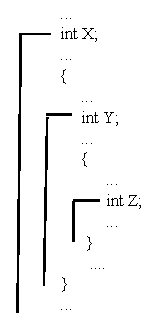
\includegraphics[width=9cm,height=6cm]{images/scope1.eps}}
\setlength{\unitlength}{1cm}
\begin{picture}(10,3.3)
\linethickness{0.3mm}

%\put(0.3,3.3){\line(1,0){14}}
%\put(0.3,0){\line(1,0){14}}
%\put(0.3,3.3){\line(0,-1){3.3}}
%\put(14.3,3.3){\line(0,-1){3.3}}
\put(2.5,2.8){\large{Command line: \codefont{>a.out these are args}}}
\put(2.5,2.2){\large{Resulting data structures:}}
\put(6.3,1.7){\codefont{argv[0]} \hspace*{1.5cm}  a . o u t \textbackslash 0}
\put(6.3,1.2){\codefont{argv[1]}  \hspace*{1.5cm} t h e s e \textbackslash 0}
\put(6.3,0.7){\codefont{argv[2]}  \hspace*{1.5cm} a r e \textbackslash 0}
\put(6.3,0.2){\codefont{argv[3]}  \hspace*{1.5cm} a r g s \textbackslash 0}

\put(3.5,1.8){\codefont{argc}}
\put(4.6,1.2){\codefont{4}}

\color{\mycolor}{
\put(7.8,1.8){\vector(1,0){1.3}}
\put(7.8,1.3){\vector(1,0){1.3}}
\put(7.8,0.8){\vector(1,0){1.3}}
\put(7.8,0.3){\vector(1,0){1.3}}

\put(4.5,1.1){\line(0,1){0.5}}
\put(5.5,1.1){\line(0,1){0.5}}
\put(4.5,1.1){\line(1,0){1.0}}
\put(4.5,1.6){\line(1,0){1.0}}
}
\end{picture}
\caption{Illustration of command-line arguments in C++.  This shows the data structures created when the command-line command: ``\codefont{a.out these are args}" is run.  The program name is \codefont{a.out}, the arguments are  \cf{these}, \cf{are}, and \cf{args}. The parameter \codefont{argc} gets the value 4 because there are four arguments total, including the program name (\codefont{a.out} in this example), which is also treated as an argument.  Note that \codefont{argv} is an array of pointers to C-style strings and each argument is stored as a C-style array of characters (an array of individual characters ending with the \codefont{null} character \textbackslash 0; see Interlude 5).}
\label{fig:args}
\end{figure}

Because \codefont{main()} is a function, it can both return a value and can accept arguments.  To write a C++ program that accepts command-line arguments, the \codefont{main()} function is written as:\\
\codefont{
int main(int argc, char* argv[])\footnote{Another, equivalent option is \codefont{int main(int argc, char **argv).}}\\
}
with \emph{exactly} those variable names.  The variable \codefont{argc} (short for ``ARGument Count'') is the number of arguments passed to \codefont{main()}.  The variable \codefont{argv} (short for ``ARGument Vector'') is an array of pointers to C-style character strings (see Interlude 5).   Figure~\ref{fig:args} illustrates these data structures and their contents if the program is run using the arguments listed previously.  Notice that the first string pointed to by the \codefont{argv} array is the program name, \codefont{a.out}.

Running a program called \codefont{a.out} from the command line with arguments would look like this:\\
\codefont{
>a.out these are args\\
}
where \codefont{>} is the command-line prompt and the extra arguments are \cf{these}, \cf{are}, and, \cf{args}  By default the name of the program (in this case, ``a.out'') is also passed to the program as an argument.  This allows a program to ``know'' its own name when it runs.

The projects in this text don't involve passing arguments to \codefont{main()} because many Integrated Development Environments (IDEs) don't normally use the command line.  It is always possible to run a program from the command line, but the steps vary somewhat by IDE and operating system.  For example, in a Windows environment, running a program from the command line may require opening  a command window, moving to the directory containing the compiled program (the executable), and running the program with associated arguments.  Thus, the projects in this text are designed to be used without command line arguments.

The arguments to \codefont{main()} are \emph{always} treated as C-style strings, even if they are meant to be integers.  For example, if a program is run with the command-line argument \codefont{415}, it is treated as a string of characters: \cf{415}.  To get the argument as an actual integer a function such as \codefont{atoi()} needs to be used.  The function \codefont{atoi()} is defined in the \codefont{cstdlib} (see Section~\ref{appendix:libraries} of Appendix A), is short for Ascii TO Integer, and converts a C-style string into an integer.  For example, the command:\\
\codefont{X = atoi(``415'');}\\
will change the string ``415'' into the integer \codefont{415} and store it in \codefont{X}.

Command-line arguments can be useful for setting important parameters within a program.  For example, in the NIM program, a command-line argument could be used to set the initial number of objects.  In the Electronic Pet program, a command-line argument could be used to supply the name of the pet to be played with (or the name of the file containing the pet if the program has been modified to save and reload pets).  In the Generic Board Game, a command-line argument could be used to supply the name of the game to be played (or the name of the game file to open).  Of course, all of this data could also be supplied using input/output commands when the program is running.  Command-line arguments are generally only required when one program is starting another program and can't easily respond to user-oriented input/output.

\addtocounter{chapter}{1}

\setcounter{section}{0}
\setcounter{figure}{0}

%********** Chapter 7 **********
\chapter{Linked Robots}\index{linked list}\index{projects!Linked Robots}

\section{Introduction}

This chapter introduces the final project, Linked Robots.  The program creates a dynamic data structure (a linked list) of robot objects and demonstrates a few of the capabilities of linked lists.  In particular, the ability to modify the length of the linked list, by adding and deleting data elements from it, while the program is running.  The program doesn't do very much, but it introduces the possibilities inherent in dynamic data structures and is the basis for more complex two dimensional simulations.  For example, it could be combined with the Robot World program to allow multiple robots per cell or with the Electronic Pet to allow a user to easily play with multiple pets at the same time.

This project reviews the topics from the earlier chapters, particularly classes and pointers, and introduces three new topics:
\begin{tight_itemize}
\item Dynamic data structures
  \item Linked lists
   \item Recursion
\end{tight_itemize}

A linked list is a a dynamic data structure that allows a program to create and delete an unlimited number of data elements dynamically.  Recursion is a powerful programming technique in which a function calls itself or two (or more) functions call each other.

\section{The Program}

The Linked List program requires three new files: 
the main file (Listing~\ref{listing:robotlinkedlist}), which can have any name, and two library files: ``node.h'' (consisting of  Listing~\ref{listing:nodeh} followed by
Listing~\ref{listing:nodecpp}) and ``linkedlist.h'' (consisting of 
Listing~\ref{listing:llh} followed by
Listing~\ref{listing:llcpp}).  Note that the names of the library files are used in \cf{include} statements in the other files, so can't be changed (unless the \cf{include} statements are also changed).  The file ``robot.h'' from the previous project should  also be available to the program.  As always, as the program is entered, try to figure out what the commands do.  Most of them should be very familiar by now, but some of the syntax (particularly in the code from Listing~\ref{listing:nodecpp} and Listing~\ref{listing:llcpp}) may be somewhat confusing.

\begin{minipage}{\textwidth}
\renewcommand*\thelstnumber{\the\value{lstnumber}}
\begin{lstlisting}[language=C++,numbers = left,xleftmargin=4.0ex, basicstyle=\small, emph={ll,num_robots,robot_ptr,i},emphstyle = \color{\mycolor},
showstringspaces=false,
caption = {Main program for the Linked Robots program.  The include statements (lines 4, 5, and 6) automatically include the code from the other listings.},
label={listing:robotlinkedlist}]
#include <iostream>
#include <cstdlib>
using namespace std;
#include"robot.h"
#include"node.h"
#include"linkedlist.h"
int main(){
   linkedlist ll;
   const int num_robots = 3;
   robot *robot_ptr;
   for(int i = 0; i < num_robots; i++){
        robot_ptr = new robot(i);
        ll.insert(robot_ptr);
  }
  ll.print();
  cout <<"Turn all robots left:" << endl;
  ll.turnLeft();
  robot_ptr = new robot(99);
  ll.insert(robot_ptr);
  ll.remove(2);
  ll.print();
  return 0;
}
\end{lstlisting}
\end{minipage}

%-------------------------------------  Linked list ----------------------------------------
\begin{minipage}{\textwidth}
\renewcommand*\thelstnumber{\the\value{lstnumber}a}
\begin{lstlisting}[language=C++,numbers = left,xleftmargin=4.0ex, basicstyle=\small, emph={count,head},emphstyle = \color{\mycolor},
showstringspaces=false,
caption = {The declaration of the \cf{linkedlist} class, which holds the ``head'' of the linked list.},
label={listing:llh}]
class linkedlist{
    private:
         int count;
         node *head;
    public:
         linkedlist();
         void insert(robot *);
         void print();
         void turnLeft();
         void remove(int);
};
\end{lstlisting}
\end{minipage}

\textbf{Important:} two minor changes will need to be made to the \codefont{robot} class defined in the file ``robot.h.''  First, the member function \codefont{turnLeft()} will need to be made \emph{public} (to do this, simply move the function prototype from the private to the public region of the class definition). Although it is not necessary at this point, for future changes, it may be helpful to also make \cf{turnRight()} and \cf{forward()} public as well.  Second, a new (in-line) member function will need to be added to the \cf{robot} class.  Simply add the line\\
\codefont{
int getID() \{return ID;\}\\
} 
to the public section of the \cf{robot} class.  This new function returns the ID number of a robot, and is necessary for finding a robot by its ID (so it can be removed from the linked list).

Once all of the files have been created, compile the program containing the code from Listing~\ref{listing:robotlinkedlist}.  As always, there may be some copying errors that need to be fixed.  Once the program compiles, run it and see what it does.  By carefully comparing the code to the output it should be possible to figure out much of how the linked list works.  When dealing with linked lists it is often useful to sketch what the program is doing, particularly how the list is being constructed (see Figure~\ref{fig:llillustration}).  Try doing this with the Linked Robot program as it runs.

\begin{minipage}{\textwidth}
\renewcommand*\thelstnumber{\the\value{lstnumber}b}
\begin{lstlisting}[language=C++,numbers = left,xleftmargin=4.0ex, basicstyle=\small, emph={count,head,n,temp},emphstyle = \color{\mycolor},
showstringspaces=false,
caption = {The definition of the \cf{linkedlist} class functions. },
label={listing:llcpp}]
linkedlist::linkedlist(){
    head = NULL;
    count = 0;
}
void linkedlist::insert(robot *rp){
    node *n;
    n = new node;
    n->set_data(rp);
    n->set_next(head);
    head = n;
    count++;
}
void linkedlist::remove(int n){
    if(head == NULL)
         return;
    if((head->get_data())->getID() == n){
         node *temp;
         temp = head;
         head = head->get_next();
         temp -> remove_data();
         delete temp;
         count--;
    }
    else{
         if(head->remove(n) == 1)
             count--;    
    }
}
void linkedlist::print(){
    cout << "There are " << count;
    cout << " robots in the list: \n";
    if(head != NULL)
          head->print();
}
void linkedlist::turnLeft(){
      if(head != NULL)
            head->turnLeft();
}
\end{lstlisting}
\end{minipage}

%--------------------------------------- Node -----------------------------------------------

\begin{minipage}{\textwidth}
\renewcommand*\thelstnumber{\the\value{lstnumber}c}
\begin{lstlisting}[language=C++,numbers = left,xleftmargin=4.0ex, basicstyle=\small, emph={next,data},emphstyle = \color{\mycolor},
showstringspaces=false,
caption = {The declaration of the \cf{node} class. },
label={listing:nodeh}]
class node{
    private:
         node *next;
         robot *data;
    public:
        node();
        void set_next(node *n) {next = n;}
        void set_data(robot *d) {data = d;}
        node *get_next() {return next;}
        robot *get_data() {return data;}
        void print();
        void turnLeft();
        int remove(int);
        void remove_data() {delete data;}
};
\end{lstlisting}
\end{minipage}

\subsection{Linked Lists}\index{linked list}

\begin{figure}
%\centerline{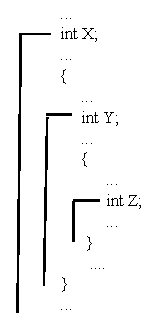
\includegraphics[width=9cm,height=6cm]{images/scope1.eps}}
\setlength{\unitlength}{1cm}
\begin{picture}(10,4)
\linethickness{0.3mm}


\put(0,3.6){\codefont{linked list object}}
\put(1.1,3.0){\codefont{head}}
\put(1.1,2.5){\codefont{count = 3}}

\color{\mycolor}{
\put(1,3.5){\line(1,0){2}}
\put(1,2.4){\line(1,0){2}}
\put(1,3.5){\line(0,-1){1.1}}
\put(3,3.5){\line(0,-1){1.1}}
\put(2.1,3.1){\vector(1,0){1.8}}

\put(4.1,3.5){\line(1,0){2}}
\put(4.1,2.4){\line(1,0){2}}
\put(4.1,3.5){\line(0,-1){1.1}}
\put(6.1,3.5){\line(0,-1){1.1}}
\put(5.1,3.1){\vector(1,0){1.7}}
\put(5.3,2.6){\vector(0,-1){1}}

\put(4.1,1.2){\line(1,0){2}}
\put(4.1,0.7){\line(1,0){2}}
\put(4.1,1.2){\line(0,-1){0.5}}
\put(6.1,1.2){\line(0,-1){0.5}}

\put(7.1,3.5){\line(1,0){2}}
\put(7.1,2.4){\line(1,0){2}}
\put(7.1,3.5){\line(0,-1){1.1}}
\put(9.1,3.5){\line(0,-1){1.1}}

\put(8.1,3.1){\vector(1,0){1.7}}
\put(8.3,2.6){\vector(0,-1){1}}

\put(7.1,1.2){\line(1,0){2}}
\put(7.1,0.7){\line(1,0){2}}
\put(7.1,1.2){\line(0,-1){0.5}}
\put(9.1,1.2){\line(0,-1){0.5}}

\put(10.1,3.5){\line(1,0){2}}
\put(10.1,2.4){\line(1,0){2}}
\put(10.1,3.5){\line(0,-1){1.1}}
\put(12.1,3.5){\line(0,-1){1.1}}
\put(11.1,3.1){\vector(1,0){1.7}}
\put(11.3,2.6){\vector(0,-1){1}}
\put(10.1,1.2){\line(1,0){2}}
\put(10.1,0.7){\line(1,0){2}}
\put(10.1,1.2){\line(0,-1){0.5}}
\put(12.1,1.2){\line(0,-1){0.5}}
}

\color{black}{
\put(4,3.6){\codefont{node object}}
\put(4.1,3.0){\codefont{next}}
\put(4.1,2.5){\codefont{data}}

\put(4,1.3){\codefont{robot object}}

\put(7,3.6){\codefont{node object}}
\put(7.1,3.0){\codefont{next}}
\put(7.1,2.5){\codefont{data}}

\put(7,1.3){\codefont{robot object}}

\put(10,3.6){\codefont{node object}}
\put(10.1,3.0){\codefont{next}}
\put(10.1,2.5){\codefont{data}}

\put(10,1.3){\codefont{robot object}}

\put(13,3.0){\codefont{NULL}}
}
\end{picture}
\caption{An illustration of a linked list.  The linked list consists of a series of \codefont{node} objects linked by pointers.  Each \codefont{node} object points to the next one in the list and to a \codefont{robot} object.  The head of the linked list is maintained by the \codefont{linked list} object, which also keeps track of the number of items in the list.  The last \cf{node} object points to \codefont{NULL}, thereby identifying the end of the linked list.  Other than the initial \codefont{linked list} object, the objects in a linked list  are usually nameless objects created with the \codefont{new} operator.  Objects can be added to or removed from the list simply by rearranging the \codefont{next} pointers.}
\label{fig:llillustration}
\end{figure}

A linked list is a \emph{dynamic} data structure.  A dynamic data structure is one in which the size of the data structure changes dynamically -- while the program is running.  In contrast an array is a \emph{static} data structure, once the size of the array is declared it cannot change size.\footnote{Part of an array could be empty, but the memory for the full array is still reserved in memory and an array can't be made larger.}  A linked list consists of a series of individual data structures ``linked'' together by pointers.  
In this program, the linked list consists of a series of \codefont{node} objects.  Each node object has a pointer called \codefont{next}, which points to the next node in the list, and a pointer called \codefont{data}, which points to the \codefont{robot} object associated with that node.  Figure~\ref{fig:llillustration} illustrates this idea.  In this example the beginning of the linked list is maintained by a separate \codefont{linked list} object.

\begin{minipage}{\textwidth}
\renewcommand*\thelstnumber{\the\value{lstnumber}d}
\begin{lstlisting}[language=C++,numbers = left,xleftmargin=4.0ex, basicstyle=\small, emph={next,data,temp},emphstyle = \color{\mycolor},
showstringspaces=false,
caption = {The definitions of the \cf{node} class functions. },
label={listing:nodecpp}]
node::node(){  // constructor
        next = NULL;
        data = NULL;
}
void node::print(){
        data->print();
        cout << endl;
        if(next != NULL)
              next -> print();
}
void node::turnLeft(){
        data -> turnLeft();
        if(next != NULL)
              next -> turnLeft();
        data -> print();
        cout << endl;
}
int node::remove(int n){
       if(next != NULL){
             if((next -> data) -> getID() == n){ // found the right ID
                  node *temp;
                  temp = next;
                  next = next -> next;
                  temp -> remove_data();
                  delete temp;
                  return(1);  // successfully removed
             }
            else{
                  return(next -> remove(n));  // try the next node
             }
     }
     return 0;     // given robot was never found
}
\end{lstlisting}
\end{minipage}  


Although linked lists and arrays both store a list of data elements, linked lists have several advantages over arrays.  First, because list items are created by \cf{new} and removed via \cf{delete}, the length of a linked list does not have to be determined in advance; it can change as needed as the program runs.  In addition, items can easily be added to, or removed from, the middle of a linked list by redirecting the pointers to include, or skip over, a node.  With an array, adding or removing an element from the middle of the array requires shifting all of the elements below the changed element.

Linked lists have two notable disadvantages.  First, the code for creating and manipulating a linked list is  more complicated than for an array.  However, a well-written linked list class encapsulates the complex parts of the code, making it easy to incorporate a linked list in other programs.  Second, linked lists don't allow for \emph{random access}\index{random access} the way that arrays do.  Accessing element $N$ of an array is a simple and quick operation.  Accessing element $N$ of a linked list requires ``stepping'' through the list until the $N$th element is found.\footnote{Basic linked lists require stepping through the list to find a particular element of the list.  However, more complex data structures can be created that, for example, combine a linked list with an array of pointers that point to various elements within the list.  This makes it possible to jump to a midpoint in the list.  But such hybrid structures are beyond the scope of this text.} 



\subsection{Recursion}\index{recursion}

A \emph{recursive} function is one that calls itself.\footnote{More generally, a program can have mutually recursive functions that call each other.}  To avoid infinite loops, a recursive function must have a \emph{terminating condition} that keeps the function from calling itself under some conditions.

Recursive functions are a natural method to step through dynamic data structures (like linked lists) or for programming recursively defined mathematical functions.  For example, the Fibonacci numbers can be defined by a function $f()$:\\
$\hspace*{1cm}f(0) = 0\\
\hspace*{1cm}f(1) = 1\\
\hspace*{1cm}f(N) = f(N-1) + f(N-2)\\$
(Note that the function is only defined for $N \geq 0$.)
A recursive function to calculate the $N$th Fibonacci number can be written as:\\
\codefont{
int fibb(int n)\{\\
\hspace*{0.5cm}if(n == 0)\\
\hspace*{1.0cm}return 0;\\
\hspace*{0.5cm}if(n == 1)\\
\hspace*{1.0cm}return 1;\\
\hspace*{0.5cm}return( fibb(n-1) + fibb(n-2) );\\
\}\\
}
The computer function almost perfectly copies the mathematical formula; it returns 0 for 0 and 1 for 1, and otherwise it returns the sum of the previous two Fibonacci numbers.  The function correctly calculates the zeroth and first Fibonacci numbers directly by returning the correct values.  For the second Fibonacci number the final return statement calls the functions \codefont{fibb(1)} and \codefont{fibb(0)}, which return the correct values, which in turn are summed and returned as the answer.

For the third Fibonacci number the return statement calls the functions \codefont{fibb(2)} and \codefont{fibb(1)}.  The function call \codefont{fibb(1)} simply returns a 1.  The function call \codefont{fibb(2)} calls the \codefont{fibb()} function twice more (with arguments 1 and 0).   Those function calls return the correct values (1 and 0), which are summed together (to give 1) and then returned to the original \codefont{fibb(3)} function to become part of the correct answer (1 + 1 = 2).  

In general, if a call is made to \codefont{fibb($N$)}, that function calls \codefont{fibb($N-1$)} and \codefont{fibb($N-2$)}.  Eventually (because each successive  call reduces the value of $N$), calls are made to
\codefont{fibb($0$)} and \codefont{fibb($1$)}, the correct answers are returned and summed repeatedly, until the correct answer is generated.

Recursion is a very powerful programming technique because seemingly complex problems can be reduced to fairly simple code.  However, it can also be slow when compared to a loop.  Thus, the decision of whether to solve a particular program problem with a loop or with recursion generally involves weighting the benefits of simplicity versus computational time.

\section{Analysis of the Code}

\begin{wrapfigure}{R}{0.5\textwidth} \framebox[\linewidth][l]{\parbox{0.95\linewidth}{\codefont{Data Structure Trade-offs} \\
A fundamental challenge in computer programming is deciding what type of data structure to use for a given problem.  With arrays, a program can quickly access any element in the array based on its index.  However, changing the size of an array or adding or removing elements from the middle of an array is difficult.  In contrast, linked lists can grow and shrink very easily and elements can be added or removed from the middle of a linked list fairly quickly, but accessing a particular element is slow compared to an array.  So, which data structure should be used?  The answer depends on the nature of the problem.  If the data is fairly static, then an array is probably best, but if elements are often being added or removed, especially if they are being added or removed from the middle of the data structure, then a linked list is often more effective.  Many other dynamic data structures have been defined, each with their own strengths and weaknesses, but those structures are beyond the scope of this text.
}}
\vspace{-1.2cm}
\end{wrapfigure}

Taking the opposite approach as in the last chapter, in this chapter, the code is analyzed in a \emph{top-down} fashion, starting with \codefont{main()} and then working ``down'' through the classes.  Looking at the code in this order can be helpful in understanding how the overall program works, before worrying about the individual details.



The program begins by creating a list of \codefont{robot} objects.  It then manipulates the robots in the list, prints them, adds robots to the list, and removes robots from the list.  
The current program can only be used to create a linked list of \codefont{robot} objects, which makes it overly specialized.  A much better linked list would allow the linked list to be used to create lists of any types of objects.  However, creating a generalized linked list requires techniques that are beyond the scope of this text, so the simpler, specialized linked list is used.

\mysubsubsection{Lines 1-6: \#includes}

Lines 1-3 include some familiar libraries.  Line 4 includes the \cf{robot} class used in the previous project; now that the \cf{robot} class has been created, it's easy to include robots in any other program.  Lines 5 and 6 include the two new classes. 

\mysubsubsection{Lines 7, 22, 23: The \codefont{main()} Function}

These lines define \codefont{main()}.

\mysubsubsection{Lines 8-10: Variable Declarations}

These lines declare the variables that will be used in the program.  Line 8 creates a linked list object called \codefont{ll}. 
Line 9 creates a constant \codefont{int} that stores the initial number of robots.   Line 10 creates a robot \emph{pointer}, which will be used to create new robot objects that will be inserted into the linked list.

\mysubsubsection{Lines 11-14: Creating the Initial Robots}

Line 11 is the beginning of a \cf{for} loop (ending on line 14) that creates \codefont{num\_robots} robots.  Line 12 creates a new \codefont{robot} object whose ID is equal to the current value of \codefont{i}.  The new \codefont{robot} object is created by the robot class's constructor (see Listing~\ref{listing:robotcpp}.)  Line 12 inserts the new robot into the linked list by calling the linked list object's \codefont{insert()} function.   

The key is that \codefont{robot\_ptr} is only a \emph{pointer} to the \codefont{robot} object.  The \codefont{insert()} function creates a new pointer to the \codefont{robot} object when it adds it to the linked list, which allows the \codefont{robot\_ptr} to be used to create another new \codefont{robot} object.  In this way, an unlimited number of robots can be created and added to the linked list.

\mysubsubsection{Line 15: Print the Robots}

Line 15 calls the \codefont{print()} function of the \cf{linkedlist} class, which causes the list of robots to be printed.   Notice in the output that the robots are printed 2, 1, 0.  This occurs because the \codefont{insert()} function ``pushes'' each robot onto the front of the list.  Thus, the last robot inserted into the list is actually the one at the front of the list.  Each robot's direction is 0 (North) and energy is 50, because they were just created.

\mysubsubsection{Lines 16-21: Manipulating the Robots}

Line 16 is just an output statement.  Line 17 makes all of the current robots turn left.  The \codefont{turnLeft()} function also prints the robots after they've turned.   Including an output statement in another type of function is generally not a good idea -- output should be reserved for the function meant to generate it (i.e., the \codefont{print()} function).  Here, the output is included in the \codefont{turnLeft()} function to illustrate how it works.

There are two important things to notice about how the robots are printed by the \codefont{turnLeft()} function.  First, they have turned left, their direction is all 3, and they've lost 1 energy.  Second, they are printed in the opposite order as in the \codefont{print()} function.  This is discussed later in this chapter, where the \codefont{turnLeft()} function is analyzed.

Lines 18 and 19 create another new robot with ID 99 and insert it into the list.  Line 20 removes the robot with ID 2 from the list and deletes it.  Then line 21 prints the new list of robots.  Notice that the last added robot (number 99) is at the front of the list, it hasn't turned left (it was added after the turn left operation) and robot number 2 is gone.

\subsubsection{Listings~\ref{listing:llh} and~\ref{listing:llcpp} : The \cf{linkedlist} Class}

The \cf{linkedlist} class defines an object that keeps track of the first element in the linked list, often referred to as the ``head'' of the list.  It also keeps track of the number of items in the list.

\mysubsubsection{Lines 1a-11a: The \cf{linkedlist} Class Declaration}

Lines 1a-11a declare the \cf{linkedlist} class.  It has two (private) data members: \codefont{count}, which keeps track of the number of items in the list; and \codefont{head}, which is a pointer to a \cf{node} object and points to the first item in the list.  If the list is empty, \cf{head} should point to \codefont{NULL}.
The class also has five (public) member functions, including the constructor. 

\mysubsubsection{Lines 1b-4b: The Constructor}

The constructor is called when a new \cf{linkedlist} object is created.  It sets the \codefont{count} to 0 and the \codefont{head} to point to \codefont{NULL}.  Having the \codefont{head} point to \codefont{NULL} is actually very important because many of the functions test for \codefont{NULL} before trying to access the list -- if the \codefont{head} is \codefont{NULL}, these functions don't proceed because the list is currently empty.  Not checking for \codefont{NULL} before attempting to modify the linked list can lead to significant run-time errors.

\mysubsubsection{Lines 5b-12b: The \codefont{insert()} Function}

The \codefont{insert()} member function is used to insert new \codefont{robot} objects into the list.  Functions like this are also often called \codefont{push()}  because they ``push'' an item onto the beginning of the list.  The function's parameter is a pointer to the \codefont{robot} object to be inserted in the list. Thus, on line 13, the \codefont{insert()} function is called with \codefont{robot\_ptr}, which is a pointer (line 10).

Line 7b creates a new \codefont{node} object.  Line 8b calls the \codefont{set\_data()} member function of the node class, which makes the new \codefont{node} object point to the \codefont{robot} object.  Note that the \codefont{set\_data()} function is called using the arrow notation (\codefont{-$>$}) rather than the dot notation (.) because \codefont{n} is a pointer to a node, not a node itself.

Line 9b makes the new \codefont{node} object point to the same thing as the \codefont{head} pointer.  At this point both \codefont{head} and the new node's \codefont{next} data member (line 3c) are pointing to the first element in the linked list (which could be \codefont{NULL} if the list was empty). 

Now, line 10b makes \codefont{head} point to the new \codefont{node} object.  The new node has been inserted into the list between the \codefont{head} and the previous first element of the list.  

Finally, line 11b increases the \codefont{count} by 1 because a new element has been added to the list.

\mysubsubsection{Lines 29b-38b: The \codefont{print()} and \codefont{turnLeft()} Functions}

The \codefont{print()} member function begins by printing the number of elements in the list (lines 30b and 31b).  Then if the list is not empty (i.e., \codefont{head} isn't pointing to \codefont{NULL}) it calls the \codefont{print()} member function of the first node in the list.  This node ``prints itself'' and then recursively asks the next node to print itself (see the description of the node class's \codefont{print()} function).

The \codefont{turnLeft()} member function (lines 35b-38b) is very similar.  So long as the list isn't empty, the function simply asks the first node in the list to turn left.

\mysubsubsection{Lines 13b-28b: The \codefont{remove()} Function}

The \codefont{remove()} member function attempts to remove the robot whose ID number is \codefont{n} from the list.  It looks a bit complicated, but most of the complication occurs only if the target node is the very first element of the list.  In dealing with linked lists, and other dynamic data structures, modifications to the first (or last) element in the data structure are often a bit more complicated than modifying any other element in the structure.

Lines 14b and 15b check if the list is empty.  If it is, then there is nothing to remove, and the function simply returns.   

Line 16b checks whether the first element in the list is the robot that needs to be removed.  The syntax of the conditional is a bit tricky:\\
 \codefont{((head->get\_data())->getID() $==$ n)}\\
  It starts with the \codefont{head} variable, then the \codefont{->get\_data()} gets the data (i.e., the robot) of the first element of the list by following the \codefont{head} pointer.  Then the \codefont{->getID()} gets the ID of the robot.  Finally, this ID is compared to the target ID (which is \codefont{n}).  If the IDs match, meaning that the first robot is the one to be removed, then the \codefont{head} pointer has to be changed to point to the second element in the list, thereby skipping over, and effectively removing, the first element of the list.  Lines 17b and 18b create a temporary pointer and point it to the first element in the list.  Line 19b makes \codefont{head} point to the second element in the list (by setting it equal to the element after the first one).  Line 20b tells the node to delete the \codefont{robot} object from memory, and line 21b deletes the node from memory.  Without these two lines, the node and robot would remain in memory, but with nothing pointing to them and no way to access them, thus wasting memory.   Finally, line 22b adjusts the count.

If the first element is not the one to be removed, then line 25b calls the \codefont{remove()} member function of the \cf{node} class (described in detail below).  This function will recursively step through the linked list looking for the right element to remove.   In addition to calling the \codefont{remove()} function, line 25b compares whatever the function returns to the value 1.  If the \codefont{remove()} function is successful, it returns the value 1, and the linked list object reduces its count by 1 (line 26b).  If the \cf{node} class's \codefont{remove()} function was unsuccessful, it returns a 0 and the count remains unchanged.

\subsubsection{Listings~\ref{listing:nodeh} and~\ref{listing:nodecpp}: The \cf{node} Class}

The \cf{node} class defines the individual node objects that make up the linked list.  Each node object points to a robot object and points to the next node in the list, except for the last node in the list, which points to \codefont{NULL}.

\mysubsubsection{Lines 1c-15c: The \cf{node} Class Declaration}

Lines 1c-15c declare the \cf{node} class, which consists of two private data members and nine public member functions, including a constructor.  

Five of the member functions of the \cf{node} class are in-line functions.  The functions \codefont{set\_next()}  (line 7c) and \codefont{set\_data()} (line 8c) simply allow the \codefont{next} and \codefont{data} members to be set.  Notice that both take pointer arguments because \codefont{next} and \codefont{data} are both pointers.  Similarly, the functions \codefont{get\_next} and \codefont{get\_data()} return a pointer to the next node in the list and a pointer to a node's data, respectively.\footnote{Given that these functions make the data members of the \cf{node} class fully accessible, it would not be unreasonable to simply make \codefont{next} and \codefont{data} public.  This would make the \cf{get()} and \cf{set()} functions unnecessary.  However, for this project, we'll stick with the idea that data members should be private.}  The last in-line function is \codefont{remove\_data()}.  This function deletes the \codefont{robot} object that the \codefont{node} object is pointing to and is used as part of the remove operation.

\mysubsubsection{Lines 1d-4d: The Constructor}

When a new \codefont{node} object is created the constructor sets its pointers to \codefont{NULL}.

\mysubsubsection{Lines 5d-10d: The \codefont{print()} Function}

This function uses recursion to step through all of the elements in the linked list, printing them as it goes.  First, line 6d makes the \codefont{data} of the current node ``print itself'' by calling its \codefont{print()} function.  Because \codefont{data} is pointing to a \codefont{robot} object, this calls the \cf{robot} class's \codefont{print()} member function (Listing~\ref{listing:robotcpp}, line 29b).   The arrow (\codefont{->}) notation is used rather than the dot notation (.) because \codefont{data} is a pointer.  Next, a new line is printed (line 7d).  Then the function checks whether there is another node in the linked list (line 8d).  If \codefont{next} is \emph{not} pointing to \codefont{NULL}, it means that there is another node in the linked list and that node's \codefont{print()} function is called (line 9d).  

It's important to understand how the \codefont{print()} function works.  Even though the linked list can contain many elements, an explicit loop is not necessary to access them all.  Instead, it is sufficient for each node to print itself and then ask the next node in the list to do the same thing.

\mysubsubsection{Lines 11d-17d: The \codefont{turnLeft()} Function}

The \codefont{turnLeft()} function has a similar structure to the \codefont{print()} function.  First, the node tells the robot to which it is pointing to turn left (line 12d).  Then the function checks whether there's another node in the linked list (line 13d).  If there is, then the function calls that node's \codefont{turnLeft()} function.  So, the \codefont{turnLeft()} function of every node in the linked list is eventually called.

Next, lines 15d and 16d have each node's robot print itself and then print a new line.  

Notice that the \codefont{print()} and \codefont{turnLeft()} functions print the robots in \emph{opposite} order (reexamine the output to double check this).  Because of the way the \codefont{insert()} function works, the robots are pushed onto the front of the linked list.  So, when \codefont{main()} adds the robots (0, 1, 2) they actually end up on the linked list in the order 2, 1, 0, with robot 2 closest to the head of the list.  

To understand how the \codefont{turnLeft()} function prints the robots in the opposite order from the \cf{print()} function, look at Figure~\ref{fig:llillustration}.  In the \codefont{turnLeft()} function, the first node in the list begins by having its own robot turn left (line 12d).  Then it calls the next node's \codefont{turnLeft()} function (line 29c).  This causes the program to jump to that node's \codefont{turnLeft()} function.  Only when that function is done executing and returns does the program come back to the first node's \codefont{turnLeft()} function and execute lines 15d and 16d, printing the robot.  Thus, the first node's robot turns left \emph{before} any of the other robots, but it gets printed \emph{after} all of the other nodes are finished with their \codefont{turnLeft()} function and have returned.

The printing order in the \codefont{print()} function can be reversed simply by moving lines 6d and 7d to after line 9d.  This will cause the robots that are later in the linked list to get printed \emph{before} the robots that are earlier in the list.  Similarly, the printing order in the \codefont{turnLeft()} function can be reversed by moving lines 15d and 16d to before line 13d.

%Make sure that the difference between the printing order in the \cf{turnLeft(0} function and the \cf{print()} function is clear.  Clearly understanding how these functions print the robots in linked list in different orders will help you understand linked lists in general.

\mysubsubsection{Lines 18d-33d: The  \codefont{remove()} Function}

The \codefont{remove()} member function finds a particular node using the ID number and removes it from the linked list.  Removing an item from a linked list is simply a matter of getting the node before the node that's being removed to point to the node that comes after the one that's being removed.  Thus, the linked list pointers ``jump over'' the removed node, effectively removing it from the linked list.  The node and data of the removed node should be deleted so they don't remain in memory.

Line 19d makes sure that the next node isn't \codefont{NULL}.  If it is \codefont{NULL}, then the end of the linked list has been reached, the desired node wasn't found, and a 0 (for no node deleted) is returned (line 32d).
If the next node is not \codefont{NULL}, then line 20d checks the ID of the next \codefont{robot} to see if it matches the target number.  If it doesn't, then the next node's \codefont{remove()} function is called (line 29d) to try to find (and remove) the node from farther down the list.    

If the next node does point to the robot with the target ID, the first step is to create a node pointer called \codefont{temp} (line 21d).  This pointer is pointed at the next node (line 22d), the one to be removed.  The \codefont{temp} pointer will act as a temporary reference to the \codefont{node} object being removed from the list, so that it can be deleted.  Then the current node is changed to point to the node two places down the list:\\
\codefont{next = next $->$ next;}\\
This effectively cuts the target node out of the list.  Line 24d uses the \codefont{temp} pointer to delete the target \codefont{robot} object, and line 25d uses the \codefont{temp} pointer to delete the \codefont{node} object that was pointing to the target \codefont{robot} object.  Without the \codefont{remove\_data()} and \codefont{delete} function calls, the node and robot would remain in memory, but they would be inaccessible (because nothing would be pointing to them).  This would cause a ``memory leak'' -- an error in which memory wasted by being allocated to store some data, but is not released when the data is no longer needed.

\vspace{+0.25cm}
{\color{\mycolor}\noindent\hrulefill}
\section{Exercises: Modifying the Program}

Linked lists (and other similar dynamic data structures) are designed to make it as easy and efficient as possible to manipulate (add, remove, find, rearrange, etc.) the data elements in the structure.  Thus, most of the changes to the Linked List project involves adding more functions to manipulate the data.

\mysubsubsection{Exercise 1: Changing the Print Order}

Reverse the order that the \codefont{print()} function prints the robots in.  This can be done by simply moving the print commands on lines 6d and 7d to follow line 9d.  


\mysubsubsection{Exercise 2: More Actions}

Currently, the robots in a linked list can only turn left or be printed.  Modify the linked list and node classes to allow the robots to take turn right and to move forward.

\mysubsubsection{Exercise 3: Adding Elements at the Other End of the List}

Create a new function to add elements to the tail of a linked list.\footnote{If elements are added only to the tail and removed  from only the head, the resulting data structure is known as a \emph{queue}\index{queue}.} To do this efficiently the \cf{linkedlist} class should have an extra data member that points to the last element of the list (e.g., a \codefont{tail} pointer).  This requires modifying the constructor (to set up the tail pointer properly), the \codefont{insert()} function to adjust the \codefont{tail} properly when the first element is added to the list, and the \codefont{remove()} function to adjust the \codefont{tail} properly when the last element is removed from the list.  

Carefully check that the new \codefont{tail} function properly remains pointing to the last element in the list, regardless of how elements are inserted or removed.  

Once it is clear that the new tail pointer works properly, a new function can be created to use the \codefont{tail} pointer to add new elements to the end of the linked list.  The current \codefont{insert()} function can be used as a template for the new function.  

(A \codefont{tail} pointer is not strictly necessary for this addition.  Instead, every time an element is added to the end of the list, the new functions could step to the end of the list and then add the new element.  But for long lists, this is a very wasteful approach because of the time required to step to the end of the list.)


\mysubsubsection{Exercise 4: Individual Actions}

Create a new function that combines the \codefont{remove()} and \codefont{turnLeft()} functions that allows a specific robot to turn left.  The function should take an ID number as input, find that robot, and have it turn left.  Next create similar functions to allow individual robots to turn right and move forward.


\mysubsubsection{Exercise 5: Returning a Robot} 

Add a function that is able to search for a robot (e.g., by ID) in the linked list and return a pointer to the robot if it is in the list (or \codefont{NULL} otherwise).  The basics of this operation are very similar to the \codefont{remove()} operation, as it requires stepping through the list to find the robot with the correct ID.   However, instead of removing the element and returning a 0 or 1, the function would return a \emph{pointer} to the robot.  

\section{Problems}

\begin{enumerate}[{\bf 1.}]

\item {\bf The Robot World}\\
 Combine the linked list of robots with the Robot World program to allow multiple robots to occupy the same square.  Instead of maintaining a two-dimensional array of pointers to robots, the \cf{world} class could maintain a two-dimensional array of linked lists.  As a robot moves from square to square it is removed from one list and added to the next.

\item {\bf Doubly linked lists}\\
 Create a doubly linked list, in which each node in the list has a pointer to both the next node in the list and the previous node in the list.  Doubly linked lists allow a list to be traversed in either direction and can significantly speed up many operations.  Creating a doubly linked list requires adding a new pointer to the node class to point to the previous node in the list and modifying the existing \codefont{insert()} and \codefont{delete()} functions to correctly redirect the new pointer.

\item {\bf A linked list of pets}\\
 Linked lists can store any type of data.  Create a linked list for the pet objects from Chapter 4.  Then use it in the Electronic Pet program to allow a user to create and interact with more than one pet at a time.  It may be helpful to move the selection menu into the pet class and add a new menu that begins by asking the user for the name of the pet the want to interact with.  First, the user selects, by name, the pet to play with.  Then the program searches the linked list to find that pet, which  prints its own interactive menu.  

\item {\bf File I/O}\\
Add functionality so that a list of robots can be saved to a file and read from a file.  This means saving the data about the robots, their ID, direction, etc., in order to the file and being able to read it from a file to recreate the list.  The save function should probably be a recursive function similar to the current \cf{print()} function.  The read function should loop until the end of the file is reached.  On each loop it should read the data for one robot from the file, construct the robot, and add it to the linked list.

\end{enumerate}

%\addtocounter{chapter}{1}

\appendix
%\renewcommand\thechapter{}
%\renewcommand\thesection{\arabic{section}}
%\addtocounter{chapter}{1}
%********** Appendix **********
\chapter{Reference}

\section{Variables and Types}\label{appendix:types}

Computer programs use variables to store data.  A \emph{variable} can be thought of as a box with a name that contains a value -- the data.  Before a variable is used, it must be declared.  The basic variable declaration consists of two parts: the type and the variable name.  For example, the command:\\
\codefont{
int radius; \\
}
declares a variable of type \codefont{int}, which is short for \emph{integer} and whose name is \codefont{radius}.  It can be thought of as a box named \codefont{radius} that can contain an integer number.  

The type is important for several reasons.  
\begin{enumerate}
\item The type determines how big the ``box'' that holds the data needs to be (e.g., a single character takes up less space in memory than a real number).   
\item The type determines how to interpret the data stored in the ``box'' -- all data is fundamentally stored as a binary number (i.e., a series of 1's and 0's), but how the number is interpreted depends on the data's type.  
\item The type determines how operations should be applied to the data stored in the ``box.''  For example, if the division operation is applied to two real numbers it returns a real number, but if it is applied to two integers, it truncates the answer and returns an integer.
\end{enumerate}

The most commonly used types in C/C++ are introduced in Table~\ref{tab:types}.

There are several commonly used forms a of variable declaration:\\
\cf{
int x;\\
int v1, v2, v3;\\
int v = 7;\\
}
The first example simply declares a single variable called \cf{x}.  The second example is a multiple declaration that declares three variables, all of type \cf{int}, named \cf{v1}, \cf{v2}, and \cf{v3}.  Any number of variables can be declared in one line as long as they all have the same type.  The third example declares a variable named \cf{v} and assigns it the initial value 7.  It's often a good idea to assign variables an initial value, otherwise the variable's value is undefined, which may cause errors if an attempt is made to use the variable's value without setting it somewhere else in the program.\footnote{Many languages require all variables to be assigned an initial value, assign variables a default initial value such as zero, or check that a variable has been assigned a value before the variable can be used.  C++ does none of these things, instead leaving it up to the programmer to make sure that variables are assigned reasonable values before they are used.}


\begin{table}
\centering
\caption{Common Variable Types in C++.  Note that the actual number of bytes used to store a variable, and hence the allowed range of the variable, may vary from system to system.}
\begin{tabular}{|  p{1.5cm}  | p{2.5cm} | l |p{2.5cm}| p{6.5cm}|}
\hline
\textbf{Type} & \textbf{Name} & \textbf{Size(bytes)} & \textbf{Range} & \textbf{Description} \\
\hline
\codefont{int} & Integer & 4&  -2147483648 to 2147483647  & Variable holding an integer number; a positive or negative number without a decimal. \\
\hline
\codefont{short int} (or \codefont{short}) & Short integer & 2&  -32768 to 32767  & Variable holding a short integer number; a positive or negative number without a decimal. \\
\hline
\codefont{long int} (\codefont{long}) & Long integer & 4 &   -2147483648 to 2147483647  & Often the same as an integer; may be larger, for example, on a 64-bit machine. \\
\hline
\codefont{float} & Floating point & 4 & $\pm3.4e^{\pm38}$ ($\sim$7 digits of precision) &  Variable holding a positive or negative real number.  Floating-point numbers are stored using an exponent, which allows the decimal place to ``float.'' \\
\hline
\codefont{double} & Double-precision floating point & 8 & $\pm1.7e^{\pm308}$ ($\sim$15 digits of precision) &  Often the same as a \cf{float}, but may use 16 bytes. \\
\hline
\codefont{long double} & Long double-precision floating point & 8 & $\pm1.7e^{\pm308}$ ($\sim$15 digits of precision) &  Often the same as a \cf{double}; may be larger depending on the machine it's running on. \\
\hline
\codefont{char} & Character & 1 & 0 to 255 &  Stores a single character (`a', `b', `4', `\$', `+', etc.). \\
\hline
\codefont{unsigned} & Unsigned number & Varies & Varies & The modifier \cf{unsigned} can be applied to \cf{int}s (including long and short \cf{int}s).  It makes the number unsigned (always positive) and doubles the maximum range of the variable.  For example, an unsigned \codefont{int} has a range of 0 to 4294967295.\\
\hline
\end{tabular}\label{tab:types}
\end{table}

\subsection{Naming Variables}

Variables should be given names that make it easier to read the program.  For example, variable names from the first two projects include: \cf{lucky} for the user's lucky number, \cf{favorite} for the user's favorite integer, and \cf{num\_objects} for the number of objects remaining in the game of NIM.  

The rules for valid variable names are fairly simple.  Variable names can use letters, underscores (\_), and digits, but cannot start with a digit and must contain at least one letter.   They may not be a reserved word, such as \codefont{if}, \codefont{int}, or \codefont{main}.  Case matters in variable names: \codefont{Lucky} is not the same variable as \codefont{lucky}.  Legal variable names include: \codefont{X}, \codefont{a\_variable}, and \codefont{variable7}, but \emph{not} \codefont{7variable} (starts with a digit), \codefont{\_123} (doesn't contain a letter), or \codefont{do} (a reserved word).  There are a number of conventions for choosing variable names and software companies often enforce the use of a particular convention.  Several  conventions are used in this text to demonstrate the range of variable naming styles.

%Other Appendices:

%\section{I/O: cin, cout, files}


\section{Conditionals: \codefont{if, if-else, switch}}\label{appendix:conditionals}
 % ------------------------------------ conditionals ---------------------------

\emph{Conditionals} are commands that allow a program to take different actions depending on specific conditions.  The most common conditionals in C++ are \codefont{if},  \codefont{if-else}, and \codefont{switch}.

The structure of an \codefont{if} statement is\\
\codefont{
if(\emph{condition}) \{\\
\hspace*{0.5cm}Execute this block of code\\ 
\hspace*{0.5cm}if the condition is true\\
\}\\
Always executed\\
}
If the condition in the  \codefont{if} statement is, or evaluates to, zero, it is treated as false; otherwise, it is treated as true.  Thus, the condition can be anything that C++ can interpret as an integer.  However, to make programs readable, the condition should generally be a test of some kind, such as  \codefont{ X $<$ Y}, which is true if \codefont{X} is less than \codefont{Y} and false otherwise.

The structure of an \codefont{if-else} statement is:\\
\codefont{
if(\emph{condition}) \{\\
\hspace*{0.5cm}Execute this block of code 
\hspace*{0.5cm}if the condition is true\\
\}\\
else \{\\
\hspace*{0.5cm}Execute this block of code otherwise\\
\}\\
Always executed\\
}
In both conditionals, the curly brackets defining the block after the \codefont{if} and the \codefont{else} may be omitted if only a single command is used after the  \codefont{if} or the \codefont{else}.  For example,\\
\codefont{
if(condition)\\
\hspace*{1cm} Single command to be executed\\
Always executed\\
}
However, it is good programming practice to include the curly braces, even when they are not  necessary.  It makes the code easier to read and avoids potential errors if additional commands are added to the \cf{if} or \cf{else} clause.

% switch ---------------------------------------------------------

The switch statement allows a program to make multiple decisions based on an integer or character value.  The basic structure of a switch statements is:\\
\codefont{
switch(\emph{variable} of type int or char)\{\\
\hspace*{0.5cm}      case 1:\\
\hspace*{1.0cm}  code block 1\\
\hspace*{1.0cm} break;\\
\hspace*{0.5cm}   case 2:\\
\hspace*{1.0cm}  code block 2\\
\hspace*{1.0cm}   break;\\
\hspace*{0.5cm}    ...\\
\hspace*{0.5cm}    default:\\
\hspace*{1.0cm}  code block N\\
\hspace*{1.0cm}   break;\\
\}\\
}
The program examines the value stored in the \codefont{variable} and jumps to the matching case.  For example, if the \codefont{variable} has the value 2, then the program jumps to case 2.  If none of the cases match, then the program jumps to the default case.  (A default case is not required; if one is missing and the \codefont{variable} value doesn't match any other case, the \codefont{switch} is simply skipped.)  Once the program reaches a case, it continues to execute instructions sequentially, including later cases.  Thus, the \codefont{break} statement is included, which causes the program to jump to the end of the switch statement instead of continuing to the other cases.

Generally the \cf{variable} is an integer, as shown in the example.  Alternatively the \cf{variable} could by a \cf{char} in which case the cases should be labeled with characters in single quotes, such as \cf{case: 'a'}.\footnote{
The \cf{variable} can be an expression that evaluates to either an integer or a character, in which case the program evaluates the expression and jumps to the case matching the result.  However, this can make for very confusing code.  If an expression is necessary it's better to include it as a separate line of code before the switch statement and store the result of the expression in a variable that's used to control the switch.}  


% ---------------- Loops --------------------------------------
\section{Loops: \codefont{for}, \codefont{while}, \codefont{do-while}}\label{appendix:loops}

\emph{Loops} allow a program to execute the same block of code repeatedly.  Without loops, writing repetitive programs would be extremely tedious (even with cut and paste).  The three common types of loops in C++ are  \codefont{do-while}, \codefont{while}, and \codefont{for}.  

The \cf{do-while} loop is used when the code within the loop should be executed at least once.    The basic structure of a  \cf{do-while} loop is\\
\codefont{
do\{\\
\hspace*{0.5cm} Execute this code the first time and \\
\hspace*{0.5cm} while the condition is true\\
\}while(\emph{condition});\\
Jump to the code here when the condition is false\\
}
Because the condition comes at the end of the loop, the code within the loop is executed at least once before the condition is checked.  
 
The basic structure of a  \cf{while} loop is:\\
\codefont{
while(condition)\{\\
\hspace*{0.5cm} Execute this code while the condition is true\\
\}\\
Jump to the code here when the condition is false\\
}
The condition comes at the beginning of the loop, so if the condition is false the first time it is tested, the statements within the loop won't be executed.

\cf{For} loops are generally used for ``counting'' tasks, doing something $N$ times.  The basic structure of the \cf{for} loop is\\
\codefont{
for(statement 1;  \emph{conditional};  statement 32)\{\\
\hspace*{0.5cm} Execute this code while the condition is true\\
\}\\
Jump to the code here when the condition is false\\
}
For loops are generally controlled by a \emph{counter} variable that is used to determine how many times the loop will be executed.
\codefont{Statement 1} is the \emph{initializer}, it is executed when the loop begins and is used to initialize the counter variable for the loop.  The \codefont{condition} is checked at the beginning of each loop, if it is true the loop code is run and if its false the loop is exited and the program jumps to the code after the loop. \codefont{Statement 2} is executed at the end of each loop and is used to increment the counter variable.  

The easiest way to understand a \cf{for} loop is by example.  For example, a \cf{for} loop to print the numbers from 1 to 100 is:\\
\codefont{
for(int i = 1 ;  i <= 100 ;  i++)\{\\
\hspace*{1cm}     cout << i << endl;\\
\}\\
}
The first statement creates a new integer and sets it equal to 1, the second statement (the conditional) checks whether the counter has reached 100, and the third statement increments the counter.
 
As is usual in C++, the curly brackets defining the block after a loop statement can be omitted if only a single statement is used in the body of the loop.  

%\pagebreak
%---------------------- operations ------------------------------------
\section{Mathematical Operators}\label{appendix:operators}

Mathematical operators are simply used to perform calculations within a program.
Table~\ref{tab:operators} presents the common C++ mathematical operators.  C++ uses the standard rules for order of operation and precedence when evaluating complex expressions.  For example, multiplication and division are applied before addition and subtraction, and addition and subtraction are applied from left to right.  However, there are several reasons why it is a good idea to use parentheses in complex mathematical expressions.   First, many of the operators available in C++ are unusual (\codefont{++}, \codefont{\%}, \codefont{+=}, etc.) and their order of operation is not immediately clear.  Using parentheses guarantees that expressions are evaluated in the desired order.  Second, well-placed parentheses, and spacing, make complex expressions easier to read and understand.

In mathematical expressions with variables or literals of different types C++ will often automatically convert compatible numeric types.  Generally, C++ will convert lower precision types (e.g., \cf{int}) in to higher precision types (e.g., \cf{double}).   This is known as \emph{implicit conversion}, \emph{implicit casting}, or \emph{promotion}.  For example, the expression \codefont{9.0/5} will return the value 1.8 - the integer 5 has been promoted to a \codefont{double} to match the type of the 9.0.  

The programmer can also force C++ to \emph{temporarily} convert a type for a single operation.  For example,\\
\cf{
int x = 7;\\
cout << double(x)/14;\\
}
will print 0.5 because the \cf{x} is temporarily treated as a \cf{double}.  An equivlelent 

Caution has to be used when using implicit conversion.   The expression \codefont{9/5} will return the value 1 - both values are integers so no conversion takes place and the answer is \emph{truncated} to return an integer.  More subtly the expression \cf{1.5 * (5/9)} will return the value 0 because the operation \cf{(5/9)} is performed first and it returns 0 (no conversion is done because 5 and 9 are both integers).  Thus, it's a good idea to use explicit conversion

\begin{table}
\centering
\caption{Common C++ Mathematical Operators.}
\begin{tabular}{|  c  | c |  p{7cm} |}
\hline
%\bold{Command} & \bold{Full Name} & \bold{Description} \\
\textbf{Operation} &  \textbf{Symbol} & \textbf{Description} \\
\hline
Addition &  \codefont{+} & Addition  \\
\hline
Subtraction & \codefont{-} & Subtraction \\
\hline
Multiplication & \codefont{*} & Multiplication \\
\hline
Division & \codefont{/} & Division; division of two integers results in an integer, the decimal is truncated \\
\hline 
Modulus & \codefont{\%} & Performs division and returns the remainder\\
\hline
Increment & \codefont{++} & Increments a variable by 1; note that \codefont{x++} and \codefont{++x} have different orders of operation in compound expressions.\\
\hline
Decrement & \codefont{--} & Decrements a variable by 1; note that \codefont{x--} and \codefont{--x} have different orders of operation in compound expressions.\\
\hline
Addition assignment & \codefont{+=} & Increases a variable by the given amount; e.g., \codefont{x += 7} increases \codefont{x} by $7$. \\
\hline
Subtraction assignment & \codefont{-=} & Decreases a variable by the given amount; e.g., \codefont{x -= 7} decreases \codefont{x} by $7$. \\
\hline
Multiplication assignment & \codefont{*=} & Multiplies a variable by the given amount; e.g., \codefont{x *= 7} increases \codefont{x} by a factor of $7$ and stores the result in \codefont{x}. \\
\hline
Division assignment & \codefont{/=} & Divides a variable by the given amount; e.g., \codefont{x /= 7} divides \codefont{x} by $7$ and stores the result  in \codefont{x}. \\
\hline
Modulus assignment & \codefont{\%=} & Divides a variable by the given amount and takes the remainder; e.g., \codefont{x \%= 7} divides \codefont{x} by $7$ and stores the \emph{remainder} in \codefont{x}. \\
\hline

\end{tabular}\label{tab:operators}
\end{table}



%------------------------ Boolean ---------------------------------------
\section{Comparison and Boolean Operators}\label{appendix:Boolean}

Comparison and Boolean operators are used to compare values and to construct logical expressions.  They are almost always used to define the conditions in conditional statements and loops.
Table~\ref{tab:BooleanOperators} lists the common comparison and Boolean operators used in C++.  Boolean operators always return a 1 representing \codefont{true} or a 0 representing \codefont{false}.  Thus, a comparison such as \codefont{$7 < 9$} has the value 1, which is treated as true in conditionals.  So,\\
\codefont{cout << 7 < 9 << "\textbackslash n";}\\ would print the value 1 (not \cf{true}), but \codefont{$7 < 9$} is treated as true in Boolean operations.
 
Similarly, a comparison such as \codefont{$9 < 7$} has the value 0, which is treated as false in conditionals, and the statement
\codefont{cout << 9 < 7 << "\textbackslash n";} would print 0.  
More generally, any nonzero value is treated as \codefont{true} and a zero value is treated as \codefont{false} within conditionals.  Thus, a statement such as \codefont{if(6)} is treated as \codefont{if(true)} because 6 is not zero; and \codefont{if(6 - 3*2)} is treated as \codefont{if(false)} because \codefont{6 - 3*2} is zero.

\begin{table}
\centering
\caption{Common C++ Comparisons and Boolean Operators.}
\begin{tabular}{|  c  | c |  p{7cm} |}
\hline
%\bold{Command} & \bold{Full Name} & \bold{Description} \\
\textbf{Operation} &  \textbf{Symbol} & \textbf{Description} \\
\hline
Less than & $<$ & Is true if the left operand is less than the right operand\\
\hline
Greater than & $>$ & Is true if the left operand is greater than the right operand \\
\hline
Less than or equal  & $<=$ & Is true if the left operand is less than or equal to the right operand\\
\hline 
Greater or equal  & $>=$ & Is true if the left operand is greater than or equal to the right operand \\
\hline
Equal  & == & Is true if both operands are equal \\
\hline
Not equal & != & Is true if the operands are not equal \\
\hline
AND & \&\& & Boolean AND; is true only if both operands are true \\
\hline 
OR & $||$ & Boolean OR; is true if either operand is true \\
\hline 
NOT & ! & Boolean NOT; is true if the operand is false \\
\hline
\end{tabular}\label{tab:BooleanOperators}
\end{table}

There are a few common mistakes to avoid when using these operators.  First, in addition to the Boolean operators \&\& and $||$ C++ has operators \& and $|$.  The \& and $|$  operators perform \emph{binary} AND and OR operations, which are very different from the \emph{Boolean} operations.  If a compound conditional is not behaving as expected check that it has \&\& or $||$ and not  \& or $|$.  

A similar, common, mistake is to use a single equals sign $=$ instead of a double equals sign $==$ in a condition.  The double equal sign compares two values and returns \emph{true} (1) if they are the same and \emph{false} (0) if they are different.  The single equal sign is an assignment.  Thus, the (incorrect) statement:\\
\cf{
if(x = 7)\{\\
\hspace*{0.5cm}Execute this block of code if true\\
\}\\
}
\emph{assigns} \cf{x} the value 7 and always executes the code within the \cf{if} (because \cf{x = 7} has the value 7, which is treated as true). 

%\section{ASCII Characters}


\section{The \cf{String} Class}\label{appendix:string}

The \cf{string} class defines \cf{string} objects, which are used to store strings of characters.  Strings are useful for storing names, addresses, and other pieces of text longer than a single character.
Table~\ref{tab:strings} lists some of the more useful functions that are defined as part of the \cf{string} class.  Keep in mind that a \cf{string} object is different from a C-style string (see Interlude 5), but that the member function \codefont{c\_str()} can be used to return a C-style string from a \cf{string} object.

\begin{table}
\centering
\caption{Useful Functions Related to the \cf{string} Class.}
\begin{tabular}{|  c|  c| p{6.5cm} |}
\hline
%\bold{Command} & \bold{Full Name} & \bold{Description} \\
\multicolumn{3}{|c|}{The examples use the following definitions: } \\
\multicolumn{3}{|c|}{\codefont{char c\_str[]}} \\
\multicolumn{3}{|c|}{\codefont{string str1, str2}} \\
\multicolumn{3}{|c|}{\codefont{int N}} \\
\hline
\textbf{Operation} &  \textbf{Example} & \textbf{Description} \\
\hline
\codefont{=} & \codefont{str1 = "some characters";} & Assigns a string of characters to a \cf{string} object.\\
\hline
\codefont{c\_str()} & \codefont{str1.c\_str()} & Returns the string of characters as a C-style string. \\
\hline
\codefont{length()} & \codefont{str1.length()} & Returns the length of the string. \\
\hline
\codefont{size()} & \codefont{str1.size()} & Returns the length of the string. \\
\hline
\codefont{empty()} & \codefont{str1.empty()} & Returns true if the string is empty (length is 0); otherwise, it returns false. \\
\hline
\codefont{[int]} & \codefont{str1[N]} & Returns the character at location \codefont{N} in the string.  The first position in the string is 0, not 1.\\
\hline
\codefont{at(int)} & \codefont{str1.at(N)} & Returns the character at location \codefont{N} in the string.  The first position in the string is 0, not 1. Unlike the \codefont([]) operator, \codefont{at()} performs bounds checking and will return an error if out of bounds.\\
\hline
\codefont{find(string)} & \codefont{str1.find(str2)} & Returns the location of \cf{str2} in \cf{str1}. \\
\hline
\codefont{+=} & \codefont{str1+= str2} & Appends \codefont{str2} onto \codefont{str1}. \\
\hline
\codefont{+} & \codefont{str1 = str2 + " " + str3} & Concatenates \codefont{str3} onto \codefont{str2} and stores the result in \cf{str1}. \\
\hline
\codefont{getline(istream,string)} & \codefont{getline(cin,str1)} & Gets a string of characters (including spaces and tabs) up to a new line character from the given input stream (\codefont{cin} in the example) and stores them in the given string object (\codefont{str1} in the example). \\
\hline
\codefont{==, !=, $<$,  } & \codefont{str1 == str2} & Boolean operators that compare two strings lexigraphically. \\
\codefont{$<=$, $>$, $>=$} &&\\
\hline
\end{tabular}\label{tab:strings}
\end{table}
% --------------------------------------------------------------------------

\section{\cf{iostream} Operations}\label{appendix:iostream}

The iostream library defines classes, objects, and functions related to input and output.  
Table~\ref{tab:iostream} lists some of the functions that can be applied to \cf{iostream} objects.  Most of these can be applied to either to \codefont{cin} or to an input file or to \codefont{cout} or an output file.


\begin{table}
\centering
\caption{Useful Functions of the \cf{iostream} and \cf{fstream} classes.  Most, but not all, of these functions can be applied to \codefont{cin} or an input file or \codefont{cout} or an output file.  Many of them have variants to control the number of characters read, format of output, delimiting characters, etc.}
\begin{tabular}{|  c| p{5cm} | p{8.0cm} |}
\hline
%\bold{Command} & \bold{Full Name} & \bold{Description} \\
\multicolumn{3}{|c|}{The examples use the following definitions: } \\
\multicolumn{3}{|c|}{\codefont{char char\_str[]} // a c\_style array of characters}\\
\multicolumn{3}{|c|}{\codefont{string str}  // a string object}\\
\multicolumn{3}{|c|}{\codefont{ifstream infile} } \\
\multicolumn{3}{|c|}{\codefont{ofstream outfile} } \\
\multicolumn{3}{|c|}{\codefont{int N} } \\
\hline
\textbf{Operation} &  \textbf{Examples} & \textbf{Description} \\
\hline
\codefont{open()} & \codefont{infile.open(char\_str) \newline outfile.open(char\_str) infile.open(str.c\_str()) \newline outfile.open(str.c\_str())} & Opens a file stream (input or output) with the given name.  Note that the argument must be C-style array of characters (\codefont{char [] or char *}).  Not used with \codefont{cin} or \codefont{cout}.\\
\hline
\codefont{close()} & \codefont{infile.close() \newline outfile.close()} & Closes a file stream (input or output).  Not used with \codefont{cin} or \codefont{cout}.\\
\hline
\codefont{$>>$} & \codefont{infile $>>$ str \newline cin $>>$ str} & Gets a string of characters (up to the first whitespace character) from the input stream.  The string object \codefont{str} can be replaced with other standard types (\cf{int}, \cf{char}, \cf{double}, etc.).\\
\hline
\codefont{$<<$}  & \codefont{outfile $<<$ str \newline cout $<<$ str} & Sends the string of characters from the given \cf{string} object to the output stream. The string object \codefont{str} can be replaced with  other standard types (\cf{int}, \cf{char}, \cf{double}, etc.).\\
\hline
\codefont{get()} & { \codefont{infile.get() \newline cin.get()} }&Gets and returns a character from the input stream.  Variants allow the programmer to store the character, get multiple characters, get characters up to a delimiter, etc.\\
\hline
\codefont{ignore()} & \codefont{infile.ignore() \newline cin.ignore()} & Reads and discards the next character from the input stream.  Variants allow the programmer to ignore up to $N$ characters and/or characters up to a specific character. \\
\hline
\codefont{getline()} & \codefont{infile.getline(char\_str,N) \newline cin.getline(char\_str,N)} & Reads characters from the input stream, up to \codefont{N-1} characters or a new line character, whichever comes first, and stores them in a C-style array of characters.  Variants allow the programmer to specify the delimiting character.\\
\hline
\codefont{eof()} & \codefont{infile.eof()} & Returns true if the input stream's end of file bit has been set and false otherwise.  Only regularly used with files.\\
\hline
\codefont{peek()} & \codefont{infile.peek() \newline cin.peek()} & Returns the next character without removing it from the input stream. \\
\hline
\end{tabular}\label{tab:iostream}
\end{table}

% --------------------------------------------------------------------------

\section{Libraries}\label{appendix:libraries}

Many useful libraries have been created to extend C++.  If you are starting a project that will require lots of specialized code, for example, complex mathematical functions, the ability to manipulate vectors, or complex data structures, it's a good idea to see if an appropriate library already exists.  It's rare that a library will contain code to do exactly what you want your program to do, but there are often libraries that will provide the basic code for your program, making it much easier to write.

Table~\ref{tab:libraries} lists some of the more useful and commonly used libraries.  Many, but not all, of these are used in the text.  More information on the functions defined within these libraries can be found on-line.

\begin{table}
\centering
\caption{Some Useful Libraries.}
\begin{tabular}{|  c| p{11.0cm} |}

\hline
\textbf{Library} &  \textbf{Description} \\
\hline
\cf{cstdlib} & Contains many general purpose-functions: conversion from C-style strings to numbers, generation of random numbers, and dynamic memory management.\\
\hline
\cf{cmath} & Contains useful mathematical functions: trigonometric, hyperbolic, exponential, rounding, etc.\\
\hline
\cf{ctime} & Contains useful functions relating to time: get the current time, calculate the difference between times, convert times to strings, etc.\\
\hline
\cf{cstring} & Contains useful functions for manipulating C-style strings: concatenate strings, compare strings, search strings, etc.\\
\hline
\cf{fstream} & Defines the \cf{fstream} classes (file stream) used in C++. \\ 
\hline
\cf{iostream} & Defines the \cf{iostream} classes used in C++. \\ 
\hline
\cf{string} & Defines the \cf{string} class for C++. \\ 
\hline
\cf{iomanip} & Defines stream manipulators used in C++.  These are used for formatting output to streams, setting width, precision, scientific notation, etc. \\ 
\hline
%standard template library &  
%\hline
\end{tabular}\label{tab:libraries}
\end{table}


%%***** Appendix 2 *****************
\chapter{Structures}\label{appendix:structures}

Because C does not support classes, any program that depends on or uses classes cannot be a C program.   Thus, the \codefont{pet} class used in the Electronic Pet (Chapter~\ref{ch:pet}) project and the  \codefont{square} class used in the Generic Board Game project (Chapter~\ref{ch:boardgame}) cannot be created or used in C.  

Instead of classes C has a precursor to classes known as a \emph{structure}\index{structure} that is defined using the keyword \codefont{struct}\index{struct}.  C structures allow a programmer to group multiple data types into one compound data type. 

The basic format of a structure definition is:\\
\cf{
struct fraction\{\\
\hspace*{0.5cm} int numerator;\\
\hspace*{0.5cm} int denominator;\\
\}; \\}
This creates a new, compound type called \cf{struct fraction} that contains two \cf{ints}.

However, programmers find using the name \cf{struct fraction} awkward and so most structure definitions are actually written like:\\
\cf{
\textcolor{\mycolor}{typedef} struct fraction\{\\
\hspace*{0.5cm} int numerator;\\
\hspace*{0.5cm} int denominator;\\
\} \textcolor{\mycolor}{fraction}; \\}
Note the keyword \cf{typedef} at the beginning and the extra \cf{fraction} at the end of the structure declaration.  This redefines the type \cf{struct fraction} with the new name \cf{fraction}.\footnote{The \cf{typedef} command can be used to rename any type, for example \cf{typedef int bob;} renames the type \cf{int} as \cf{bob}.  However, there are only a few places that \cf{typedef} is frequently used, dropping the \cf{struct} from structure names is one of them.}

Now there is a \cf{fraction} type:\\
\cf{fraction f1, x, my\_fraction;}\\
declares three new variables of type \cf{fraction}.

Each of these new variables is a compound variable containing two integers.  To access the data the \emph{dot notation} is used.  For example, the commands:\\
\cf{f1.numerator = 1;\\
f1.denominator = 2;\\
}
makes the variable \cf{f1} effectively store the number 1/2.  

Similarly, printing a structure requires printing each piece of data explicitly.  for example the command: \\
\cf{
cout $<<$ f1.numerator $<<$ "/" $<<$ f1.denominator;
}\\
will print \emph{1/2}.


Functions can be written that both accept structures as arguments and return structures.  For example:\\
\codefont{fraction add(fraction, fraction)}\\
Defines a function called \cf{add()} that takes two \cf{fraction} structures as arguments and returns a \cf{fraction} structure.  Presumably, the function adds the two fractions together, but that is determined by how the function is coded.

Like most programming constructs, structures can be nested, can contain other data types, and can contain a mixture of types.  For example, in program for a fantasy game the programmer might create a structure for holding data about a player's character:\\
\cf{
typedef struct character\{\\
\hspace*{0.5cm} char[100] name;  \hspace*{1.3cm}  // character's name\\
\hspace*{0.5cm} int maxhealth;     \hspace*{1.4cm}  // maximum health\\
\hspace*{0.5cm} int currenthealth; \hspace*{0.55cm}  // current health\\
\hspace*{0.5cm} weapon currentweapon;\hspace*{0.1cm} // another structure holding weapon information\\
\hspace*{0.5cm} float armorvalue; \hspace*{0.85cm}// current armor value \\
\} character;\\
}
Now all of the information about a player's character can be stored in one variable.

Careful use of structures can greatly simplify a complex program by grouping data together.  For example, if you find yourself creating multiple functions that all have the same long parameter list it's may be a good idea to create a single structure to hold all of the data.  Then the functions can be rewritten to have one a single parameter whose type is the new structure. 




%***** Appendix 2 *****************
\chapter{Binary and Hexadecimal Numbers}\label{appendix:binary}\label{appendix:hexadecimal}\index{binary}\index{hexadecimal}\index{decimal}

Binary and hexadecimal numbers are commonly used in computer science.  Making a basic understanding of them a very useful skill.
To understand binary and hexadecimal numbers it helps to begin with a quick refresher of the decimal number system.  The decimal number system is a \emph{positional}, base-10, system.  This means that the value of a digit depends on it's place (position or column)  in the number and the places (or columns) correspond to multiples of 10.  Table~\ref{tab:decimal} illustrates the idea, digits go in the 1's place, 10's place, 100's place, etc. So, the number 243 is really 2*100 + 4*10 + 3*1.  

Although in elementary school we're taught about the one's place, the ten's place, the hundred's place, etc., the places actually correspond to powers of 10.  The 1's place is $10^{0}$, the 10's place is $10^{1}$, the 100's place is $10^{2}$, etc.\footnote{Although there is no definitive proof, it is widely assumed that the base 10 system developed because people have 10 fingers.  Originally people counted in sets of 10, e.g. 3 sets of 10 fingers, plus 4 more, which became 3*10 + 4 or 34.}

A final important fact is that the base of a number system determines how many digits are necessary.  In a base 10 system there must be 10 digits: 0 through 9, to keep track of 0 through 9 objects.  The other places (columns) are used to denote more than 9 objects.  For example, ten objects are denoted as 10, one set of ten objects and zero single objects.

The binary system (or base 2 system) is used in computer science because at the lowest level computers store two digits: 0 and 1, which  correspond to off and on.\footnote{It is possible to design a computer that uses different voltages for different values, but difficulties in getting the necessary precision makes the binary system more practical.}  With only two digits available the first three numbers (starting from zero) must be: 0, 1, 10 because there's no digit to represent a 2.\footnote{This also leads to the joke: ``There are 10 types of people in the world, those who understand binary and those who don't.''}  Thus, the second place in the binary system is the 2's place (or more properly the $2^{1}$ place), the third place is the $2^{2}$ or 4's place, etc.  Table~\ref{tab:binary} illustrates the binary system.

\begin{table}
\centering
\begin{tabular}{c | c | c | c || c  }
$10^{3}$ & $10^{2}$ &$10^1$&$10^0$&\\
 1000's &  100's & 10's & 1's & \\
\hline
8 &   2 & 4 & 3 & 8*1000 + 2*100 + 4*10 + 3*1 = 8243 \\
&& & 1 & 1*1 = 1\\
&& & \ldots & \ldots\\
&& & 9 & 9*1 = 9 \\
&& 1 & 0 & 1*10 = 10\\
\end{tabular}
\caption{The decimal system.  The places (columns) are multiples of 10.  In a base 10 system 10 digits: 0 through 9 are required, numbers larger than 9 are denoted using the other places (columns), so no additional digits are necessary.}\label{tab:decimal}
\end{table}

The binary system has two problems.  The numbers end up being long and difficult for people to use (a ``simple'' number like 165 in decimal is 10100101 in binary) and converting back and forth between binary and decimal is awkward because the places don't line up.  Writing the decimal number 7 in binary requires three binary digits: 111, but writing the decimal nine 9 in binary requires four binary digits: 1001.

\begin{table}
\centering
\begin{tabular}{ c|c | c | c || c  }
$2^{3}$ & $2^{2}$ &$2^1$&$2^0$& Decimal Value\\
 8's &  4's & 2's & 1's & \\
\hline
 1 &  1 & 0 & 1 & 1*8 + 1*4 + 0*2 + 1*1 = 13 \\
&& & 0 & 0*1 = 0\\
&& & 1 & 1*1 = 1 \\
&& 1& 0 & 1*2 + 0*1 = 2 \\
&& 1 & 1 & 1*2 + 1*1 = 3\\
& 1 & 0 & 0 & 1*4 + 0*2 + 0*1 = 4\\
\end{tabular}
\caption{The binary system.  The places (columns) are multiples of 2.  Only the digits 0 and 1 are used.}\label{tab:binary}
\end{table}

To avoid these problems computer scientists often use a hexadecimal (base 16) system.  In a base 16 system the places are $16^{0}$ (1's place), $16^{1}$ (16's place), $16^{2}$ (256's place), etc. (see Table~\ref{tab:hexadecimal}).  This introduces a digit problem.  Consider counting in hexadecimal: \\
0, 1, 2, 3, \dots, 9, what come next in hexadecimal?  \\
It can't be 10 because in hexadecimal the number 10 represents 1*16 + 0*1 = 16 objects.  The only solution is to introduce new digits to describe the numbers 10 through 15.  Rather than introducing brand new symbols computer scientists simply borrowed letters.  So, 10 (decimal) is written as \emph{a} in hexadecimal, 11 (decimal) is written as \emph{b} in hexadecimal, up to 15 (decimal), which is written as \emph{f} in hexadecimal, and then 16 (decimal) is written as 10 in hexadecimal.


\begin{table}
\centering
\begin{tabular}{ c | c | c || c  }
$16^{2}$ &$16^1$&$16^0$&\\
   256's & 16's & 1's & \\
\hline
   2 & 4 & 3 & 2*256 + 4*16 + 3*1 = 579 \\
& & 1 & 1*1 = 1\\
& & \ldots & \dots\\
& & 9 & 9*1 = 9 \\
& & a & 10*1 = 10\\
& & \dots & \ldots\\
& & f & 15*1 = 15 \\
& 1 & 0 & 1*16 + 0*1 = 16\\
& 3 & b & 3*16 + 11*1 = 59\\
\end{tabular}
\caption{The hexadecimal system.  The places (columns) are multiples of 16.  Sixteen digits are needed: 0 through 15 (decimal).  The characters \emph{a} through \emph{f} are used for the numbers 10 through 15.}\label{tab:hexadecimal}
\end{table}

It's fairly easy to get decimal and hexadecimal numbers confused: is 23 equal to 2*10 + 3*1 (decimal) or 2*16 + 3*1 (hexadecimal)?  To solve this problem C++ puts a \emph{oX} in front of hexadecimal numbers when they are printed. This shows up whenever a memory address, which are always stored as hexadecimal numbers, is printed.  For example, when the value of a pointer is printed (see Chapter 7) it is printed as a hexadecimal number.

Hexadecimal numbers have two advantages.  First, they are fairly compact and, with practice, not too hard for humans to use.  Second, they are easily converted to and from binary, because four binary places correspond to one hexadecimal place (see Table~\ref{tab:hexbin}).  That is, to convert a binary number to hexadecimal the binary number can be converted in to blocks of four binary digits, which are converted to hexadecimal independently and then recombined.  For example:\\
10101110 (binary) = 1010 1110 = a e = ae (hexadecimal)\\
The reverse is also true:\\
a27 (hexadecimal) = a 2 7 = 1010 0010 0111 = 101000100111 (binary).\\
Thus, as long as you can easily convert numbers in the range 0 to 15 between binary and hexadecimal you can convert any number between binary and hexadecimal.  

This does not work for converting between decimal values and either binary or hexadecimal.  For example,\\
10101110 (binary) = 1010 1110 $\neq$ 10 14  $\neq$ 1014 (decimal)\\
Instead conversion from binary to decimal (or hexadecimal to decimal) requires doing the conversion place by place:\\
10101110 (binary) = $1*2^{7} + 0*2^{6} + ...$ \\
which is quite a bit harder than conversion to hexadecimal.


\begin{table}
\centering
\begin{tabular}{c |  c || c | c | c | c }
         & Original number & \multicolumn{4}{c}{Separated into bytes}\\
\hline
binary &   1011 1100 1010 1110 &  1011 & 1100 & 1010 & 1110 \\
hexadecimal &  b 9 a e & b & 9 & a & e\\
decimal & 47534 & 11 & 9 & 10 & 14 \\
\end{tabular}
\caption{Conversion between binary and hexadecimal is relatively easy because four binary digits correspond to one hexadecimal digit (second row).  This doesn't work for converting to decimal values (last row).}\label{tab:hexbin}
\end{table}


% *************** Bibliography ***************
\bibliographystyle{plain}
%{\small\bibliography{CSI}}

\backmatter
\addcontentsline{toc}{chapter}{Index}
\printindex
\end{document}
